% Generálva: html/build_tex.js. Fordítás: pdflatex vagy xelatex (kétszer), vagy tectonic.
% ==================================================================
%  Infokommunikáció tankönyvek közös preambuluma (a tankönyvsablon alapján)
%  Fordítás: pdflatex, xelatex vagy lualatex (kétszer), illetve tectonic
% ==================================================================
\documentclass[a4paper,11pt,twoside,openany]{book}
\usepackage{iftex}
\ifPDFTeX
  \usepackage[T1]{fontenc}
  \usepackage[utf8]{inputenc}
  \usepackage{lmodern}
  \usepackage{textcomp}
\else
  \usepackage{fontspec}
\fi
\usepackage[magyar]{babel}
\usepackage{microtype}
\usepackage[a4paper,inner=24mm,outer=20mm,top=24mm,bottom=26mm]{geometry}
\usepackage{amsmath,amssymb,mathtools}
\usepackage{icomma}
\usepackage{xcolor}
\usepackage{tikz}
\usetikzlibrary{arrows.meta,calc,decorations.pathreplacing,positioning,patterns}
\usepackage{pgfplots}
\pgfplotsset{compat=1.18}
\usepackage{tabularx,booktabs,array,longtable}
\usepackage{enumitem}
\usepackage[most]{tcolorbox}
\usepackage{fancyhdr}
\usepackage{titlesec}
\usepackage{cancel}
\usepackage{adjustbox}
\usepackage[hidelinks]{hyperref}

% ---------- színek: csak a behelyettesítés jelzésére ----------
\definecolor{cA}{RGB}{29,95,196}    % kék
\definecolor{cB}{RGB}{192,84,0}     % narancs
\definecolor{cC}{RGB}{122,61,179}   % lila
\definecolor{cD}{RGB}{11,125,112}   % kékeszöld
\definecolor{cE}{RGB}{180,36,90}    % bíbor
\definecolor{cR}{RGB}{28,122,49}    % zöld: eredmény
\definecolor{keret}{gray}{0.35}
\definecolor{hatter}{gray}{0.95}
\newcommand{\ca}[1]{{\color{cA}#1}}
\newcommand{\cb}[1]{{\color{cB}#1}}
\newcommand{\cc}[1]{{\color{cC}#1}}
\newcommand{\cd}[1]{{\color{cD}#1}}
\newcommand{\ce}[1]{{\color{cE}#1}}
\newcommand{\res}[1]{{\color{cR}\boxed{#1}}}
\newcommand{\bh}[2]{\mbox{\(#1\;\longmapsto\;#2\)}\hspace{1.4em plus 0.5em}\allowbreak}
\newcommand{\behely}[1]{\par\smallskip{\raggedright\noindent\hangindent=2em\hangafter=1{\small\sffamily\textbf{Behelyettesítés:}}\hspace{0.8em}#1\par}\smallskip}
% a megoldási sor jellege (tétel, behelyettesítés, ...) és megjegyzése
\newcommand{\jegyzet}[2]{\par\vspace{-2pt}{\centering\footnotesize{\sffamily\scshape #1}\if\relax\detokenize{#2}\relax\else\quad #2\fi\par}\smallskip}

% ---------- matematikai rövidítések ----------
\newcommand{\ld}{\operatorname{ld}}
\newcommand{\arctg}{\operatorname{arctg}}
\newcommand{\tg}{\operatorname{tg}}
\newcommand{\sinc}{\operatorname{sinc}}
\newcommand{\F}{\mathcal{F}}
\newcommand{\eff}{_{\mathrm{eff}}}
\newcommand{\un}[1]{\,\mathrm{#1}}
\newcommand{\vect}[1]{\mathbf{#1}}
\renewcommand{\Re}{\operatorname{Re}}
\renewcommand{\Im}{\operatorname{Im}}

% ---------- dobozok ----------
\tcbset{base/.style={enhanced,breakable,sharp corners,boxrule=0.5pt,colframe=keret,colback=white,
  fonttitle=\sffamily\bfseries\small,coltitle=black,colbacktitle=hatter,left=3mm,right=3mm,top=1.5mm,bottom=1.5mm,
  before skip=8pt,after skip=8pt}}
\newtcolorbox{feladat}[1]{base,title={#1},colframe=black,boxrule=0.8pt}
\newtcolorbox{keresunk}{base,title={Mit keresünk?}}
\newtcolorbox{jeloles}{base,title={Jelölések ebben a feladatban}}
\newtcolorbox{elmelet}[1][Elméleti háttér]{base,title={#1}}
\newtcolorbox{eredmeny}{base,title={Eredmény},colframe=cR,colbacktitle=cR!10}
\newtcolorbox{figyelem}[1][Figyelem]{base,title={#1},colframe=cB,colbacktitle=cB!10}
\newtcolorbox{tipp}[1][Tipp]{base,title={#1},colframe=cA,colbacktitle=cA!8}
\newtcolorbox{rajz}[1][Rajz: ezt kell felrajzolni]{base,title={#1},colframe=cD,colbacktitle=cD!8}

% jelöléstáblázat egy feladathoz
\newenvironment{jeltabla}{\par\noindent\small\renewcommand{\arraystretch}{1.25}\tabularx{\dimexpr\linewidth-3pt\relax}{@{}>{\raggedright\arraybackslash}p{2.6cm}X>{\raggedright\arraybackslash}p{2.6cm}@{}}\toprule
\textbf{Jel} & \textbf{Jelentése ebben a feladatban} & \textbf{Érték, egység}\\\midrule}{\bottomrule\endtabularx\par}

% lépés
\newcounter{lepes}[section]
\newcommand{\lepes}[1]{\par\medskip\stepcounter{lepes}\noindent{\sffamily\bfseries\small\arabic{lepes}. lépés: #1}\par\nopagebreak\smallskip}

% ---------- TikZ: tollal rajzolható stílus ----------
\tikzset{
  toll/.style={line width=0.7pt,line cap=round,line join=round},
  vekony/.style={line width=0.4pt},
  szagg/.style={line width=0.5pt,dash pattern=on 3pt off 2pt},
  tengely/.style={line width=0.6pt,-{Stealth[length=2.2mm]}},
  nyil/.style={line width=0.6pt,-{Stealth[length=2mm]}},
  blokk/.style={draw,line width=0.7pt,minimum width=12mm,minimum height=8mm,font=\small},
}
\pgfplotsset{tollplot/.style={axis lines=middle,axis line style={line width=0.6pt,-{Stealth[length=2mm]}},
  every axis plot/.append style={line width=0.8pt,black},tick style={black},ticklabel style={font=\footnotesize},
  label style={font=\small},xlabel style={anchor=west},ylabel style={anchor=south},
  /pgf/number format/use comma,clip=false}}

% ---------- fejléc ----------
\pagestyle{fancy}
\fancyhf{}
\fancyhead[LE,RO]{\small\thepage}
\fancyhead[LO]{\small\sffamily\nouppercase{\leftmark}}
\renewcommand{\headrulewidth}{0.3pt}
\titleformat{\chapter}[display]{\normalfont\sffamily\bfseries}{\large\thechapter.\ \chaptertitlename}{4pt}{\LARGE}
\renewcommand{\chaptermark}[1]{\markboth{\thechapter.\ #1}{}}
\titlespacing*{\chapter}{0pt}{0pt}{18pt}
\titleformat{\section}{\normalfont\sffamily\bfseries\large}{\thesection}{0.8em}{}
\titleformat{\subsection}{\normalfont\sffamily\bfseries}{\thesubsection}{0.8em}{}
% a szakaszok a saját számukat (2.4, A1) a címükben hordozzák
\setcounter{secnumdepth}{0}
\setcounter{tocdepth}{1}
\setlist{itemsep=2pt,topsep=4pt}
\setlength{\parindent}{0pt}
\setlength{\parskip}{4pt}
\allowdisplaybreaks
\emergencystretch=2em
\raggedbottom

\fancyhead[RE]{\small\sffamily Infokomm példatár}
\begin{document}
\frontmatter
\begin{titlepage}
\centering
\vspace*{30mm}
{\sffamily\large BME VIK, BMEVITMAB03\par}
\vspace{8mm}
{\sffamily\bfseries\Huge Infokomm példatár\par}
\vspace{6mm}
{\sffamily\Large Gyakorlati tankönyv\par}
\vspace{6mm}
{\large Mintavételezés és kvantálás, kódolástechnika\par}
\vspace{14mm}
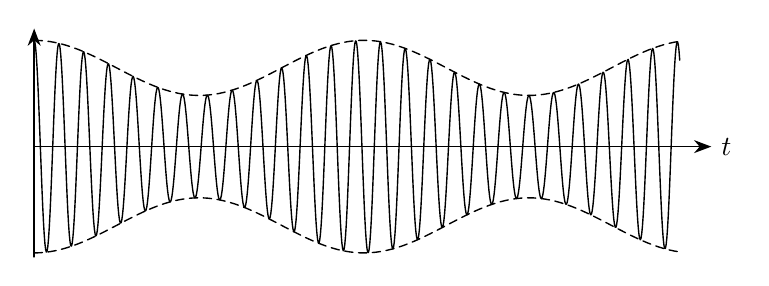
\begin{tikzpicture}[toll,x=1cm,y=1cm]
\draw[tengely] (0,-1.4) -- (0,1.5);\draw[tengely] (0,0) -- (8.6,0) node[right] {$t$};
\draw[szagg,domain=0:8.2,samples=120] plot (\x,{1+0.35*cos(\x*1.5 r)});\draw[szagg,domain=0:8.2,samples=120] plot (\x,{-1-0.35*cos(\x*1.5 r)});
\draw[line width=0.5pt,domain=0:8.2,samples=900] plot (\x,{(1+0.35*cos(\x*1.5 r))*cos(\x*20 r)});
\end{tikzpicture}
\vfill
{\small Az előadás, a gyakorlatok, a tanszéki füzet és a régi vizsgák alapján, minden eredmény újraszámolva.\par}
\vspace{8mm}
{\small 2026. november\par}
\end{titlepage}
\chapter*{Hogyan használd ezt a könyvet}
Minden feladat ugyanúgy épül fel, hogy vizsgán is ugyanebben a rendben tudj gondolkodni.
\begin{enumerate}
\item \textbf{Feladat.} A feladat szövege, alatta a forrása (vizsga, gyűjtemény, oldal).
\item \textbf{Mit keresünk?} Minden részkérdésnél leírom, melyik mennyiséget keressük, és mit jelent.
\item \textbf{Jelölések ebben a feladatban.} Minden jel jelentése abban a környezetben, ahol épp használjuk, és ha a feladat megadja, az értéke is. Ugyanaz a betű a tárgyban több dolgot is jelenthet (a $k$ lehet Nyquist-zóna sorszáma, felharmonikus sorszáma vagy erősítési tényező), ezért ezt minden feladatnál újra rögzítem.
\item \textbf{Megoldás lépésenként.} Minden matematikai sor alatt kis kapitálissal áll a sor jellege (\textsc{tétel}, \textsc{behelyettesítés}, \textsc{számérték}, \ldots) és egy rövid megjegyzés arról, honnan jön.
\item \textbf{Eredmény}, és szükség esetén \textbf{Figyelem} doboz a tipikus hibákkal, illetve a forrásban talált tévedésekkel (\textbf{Javítás}).
\end{enumerate}

\section*{A színek jelentése}
A könyv fekete-fehér, egyedül a behelyettesítést jelzem színekkel. A feladat által megadott mennyiségek közül legfeljebb ötnek saját színe van: a jelöléstáblában, a képletben a jele, a behelyettesítésnél az értéke ugyanabban a színben jelenik meg. Így ránézésre látszik, mi hova kerül.
\begin{center}
\ca{kék}\quad \cb{narancs}\quad \cc{lila}\quad \cd{kékeszöld}\quad \ce{bíbor}
\end{center}
\behely{\bh{\ca{f_H}}{\ca{75\un{kHz}}}}
\[
f_s\ge2\,\ca{f_H}=2\cdot\ca{75}=150\un{kHz}
\]

\section*{Az ábrákról}
Ahol a feladat rajzot kér, a \textbf{Rajz: ezt kell felrajzolni} doboz pontos ábrát ad, alatta pontokba szedve, hogy kézzel mit kell feltüntetni (tengelyek, jellegzetes értékek, burkoló). Minden ábra papíron egyetlen tollal is megrajzolható.

\section*{Ellenőrzés}
Minden számértéket független szkript számolt újra (\texttt{html/check}). A források hibáit a Javítás doboz és a hibajegyzék (\texttt{03\_Hibajegyzek.md}) rögzíti.

\tableofcontents
\mainmatter
\chapter*{Jelölések jegyzéke}\addcontentsline{toc}{chapter}{Jelölések jegyzéke}\markboth{Jelölések jegyzéke}{}
A tárgyban kevés betűre sok mennyiség jut, ezért ugyanaz a jel a különböző témakörökben mást jelenthet. Az alábbi jegyzék a témakörök alapjelentéseit sorolja fel. Ha egy feladatban más a jelentés, azt a feladat „Jelölések ebben a feladatban” táblázata mondja meg, és az a mérvadó.

{\small\renewcommand{\arraystretch}{1.2}\begin{longtable}{@{}>{\raggedright\arraybackslash}p{2.4cm}>{\raggedright\arraybackslash}p{8.2cm}>{\raggedright\arraybackslash}p{3.8cm}@{}}\toprule
\textbf{Jel} & \textbf{Jelentés} & \textbf{Témakör}\\\midrule\endhead
$B$ & a jel sávszélessége & Mintavétel, kvantálás\\
$B$ & a generátormátrix paritásrésze & Kódolás\\
$\mathbf B$ & a generátormátrix paritásrésze & Kódolás\\
$B_\text{be}$ & a bemenő szűrő sávja & Mintavétel, kvantálás\\
$B_\text{ki}$ & a kimenő szűrő sávja & Mintavétel, kvantálás\\
$B_\text{össz}$ & a jel teljes sávszélessége a pozitív frekvenciákon & Mintavétel, kvantálás\\
$\hat c$ & a javított (becsült) kódszó & Kódolás\\
$\hat{\mathbf c}$ & a javított (becsült) kódszó & Kódolás\\
$C$ & csúcstényező & Mintavétel, kvantálás\\
$\mathcal C$ & a kód, a kódszavak halmaza & Kódolás\\
$C_1$ & az első kód & Kódolás\\
$d_{\min}$ & kódtávolság, két kódszó legkisebb eltérése & Kódolás\\
$\hat{\mathbf e}$ & a becsült hibavektor & Kódolás\\
$f$ & a bemenő jel frekvenciája & Mintavétel, kvantálás\\
$\mathcal F$ & a forrás (forrás ABC) & Kódolás\\
$f_{AA}$ & a bemenő (antialiasing) szűrő határfrekvenciája & Mintavétel, kvantálás\\
$f_H$ & a jel legnagyobb frekvenciája & Mintavétel, kvantálás\\
$f_L$ & a jel legkisebb frekvenciája & Mintavétel, kvantálás\\
$f_R$ & a visszaállító szűrő határfrekvenciája & Mintavétel, kvantálás\\
$f_s$ & mintavételi frekvencia & Mintavétel, kvantálás\\
$f_s$ & mintavételi frekvencia (minta/s) & Kódolás\\
$f_{s,\min}$ & a legkisebb mintavételi frekvencia & Mintavétel, kvantálás\\
$G$ & generátormátrix & Kódolás\\
$\mathbf G$ & generátormátrix & Kódolás\\
$G_2$ & a második kód generátormátrixa & Kódolás\\
$H$ & a szűrő átvitele & Mintavétel, kvantálás\\
$H_\text{be}(f)$ & a bemenő szűrő átvitele & Mintavétel, kvantálás\\
$H(f)$ & a szűrő átviteli függvénye & Mintavétel, kvantálás\\
$H(\mathcal F^2)$ & a szimbólumpárok entrópiája & Kódolás\\
$H^T$ & a paritásellenőrző mátrix transzponáltja & Kódolás\\
$\mathbf H^{\mathsf T}$ & a paritásellenőrző mátrix transzponáltja & Kódolás\\
$k$ & az üzenet hossza bitben & Kódolás\\
$l$ & kódszóhossz & Kódolás\\
$L$ & átlagos kódszóhossz egy szimbólumra & Kódolás\\
$\bar L$ & átlagos kódszóhossz & Kódolás\\
$L_1$ & kódszóhossz az első forrásnál & Kódolás\\
$L_2$ & kódszóhossz a második forrásnál & Kódolás\\
$l_a$ & az a kódszavának hossza & Kódolás\\
$l_b$ & a b kódszavának hossza & Kódolás\\
$l_c$ & a c kódszavának hossza & Kódolás\\
$l_i$ & az i-edik kódszó hossza & Kódolás\\
$L^{(2)}$ & egy szimbólumpár kódszavának hossza & Kódolás\\
$n$ & a kvantáló bitszáma & Mintavétel, kvantálás\\
$n$ & a kódszó hossza bitben & Kódolás\\
$N$ & a forrás szimbólumainak száma & Kódolás\\
$N_1$ & az első forrás szimbólumainak száma & Kódolás\\
$N_2$ & a második forrás szimbólumainak száma & Kódolás\\
$n_{\min}$ & a legkisebb kódszóhossz & Kódolás\\
$p$ & egy bit hibavalószínűsége & Kódolás\\
$P$ & a jel teljesítménye & Mintavétel, kvantálás\\
$p_a$ & az a szimbólum valószínűsége & Kódolás\\
$p_A$ & az A szimbólum valószínűsége & Kódolás\\
$p_b$ & a b szimbólum valószínűsége & Kódolás\\
$p_B$ & a B szimbólum valószínűsége & Kódolás\\
$p_C$ & a C szimbólum valószínűsége & Kódolás\\
$p(0)$ & a 0 szint valószínűsége & Kódolás\\
$P(0)$ & annak valószínűsége, hogy egy bit sem hibás & Kódolás\\
$P(1)$ & annak valószínűsége, hogy pontosan 1 bit hibás & Kódolás\\
$P(2)$ & annak valószínűsége, hogy pontosan 2 bit hibás & Kódolás\\
$p(\pm1)$ & a $\pm$1 szint valószínűsége & Kódolás\\
$p(\pm2)$ & a $\pm$2 szint valószínűsége & Kódolás\\
$p(\pm3)$ & a $\pm$3 szint valószínűsége & Kódolás\\
$r$ & szimbólumsebesség (szimbólum/s) & Kódolás\\
$R$ & az ellenállás & Mintavétel, kvantálás\\
$s$ & szindróma & Kódolás\\
$s_0$ & a teljesítménysűrűség & Mintavétel, kvantálás\\
$\text{SNR}$ & jel-zaj viszony & Mintavétel, kvantálás\\
$\Delta\text{SNR}$ & a jel-zaj viszony változása & Mintavétel, kvantálás\\
$T$ & mintavételi idő & Mintavétel, kvantálás\\
$T_1$ & első mintavételi idő & Mintavétel, kvantálás\\
$T_2$ & második mintavételi idő & Mintavétel, kvantálás\\
$\hat u$ & a becsült üzenet & Kódolás\\
$\hat{\mathbf u}$ & a becsült üzenet & Kódolás\\
$U$ & a bemenő jel amplitúdója & Mintavétel, kvantálás\\
$U_{6{,}2}$ & a kimenő 6,2 kHz-es összetevő amplitúdója & Mintavétel, kvantálás\\
$v$ & a vett szó & Kódolás\\
$\mathbf v$ & a vett szó & Kódolás\\
\bottomrule\end{longtable}}
% Generálva: html/build_tex.js (ch02.js). Kézzel ne szerkeszd, a forrás a html/data mappa.
\setcounter{chapter}{1}
\chapter{\texorpdfstring{Mintavételezés és kvantálás}{Mintavételezés és kvantálás}}\label{f2}
Az analóg jelből mintasorozat, abból kódszavak, majd vissza analóg jel. A fejezet példái három kérdés köré épülnek: milyen $f_s$ mellett állítható vissza a jel, milyen álképek (alias) és szivárgó komponensek jelennek meg, és mekkora a kvantálás miatti jel-zaj viszony.

\section{Alapok, egyszerűen}
\subsection{\texorpdfstring{A1. A digitalizálás lánca, egyszerűen}{A1. A digitalizálás lánca, egyszerűen}}\label{a2-lanc}
A digitális átvitel lánca: \textbf{bemenő (előszűrő, antialiasing) szűrő $\to$ mintavevő $\to$ kvantáló $\to$ kódoló $\to$ átvitel $\to$ dekódoló $\to$ D/A (impulzusgenerátor) $\to$ visszaállító szűrő}. A digitalizálás = mintavételezés + kvantálás (ea01).

Gondolj egy filmre. A mintavételezés azt dönti el, hány képkocka készül másodpercenként, a kvantálás azt, hány árnyalattal rajzolunk egy kockát. Ha túl ritkák a kockák, a gyors mozgás hamis lesz (a kocsikerék visszafelé forog): ez az \textbf{aliasing}. Ha kevés az árnyalat, a kép szemcsés: ez a \textbf{kvantálási zaj}.

Mire jó? Minden mintavételes feladat ennek a láncnak egy-egy pontjáról kérdez: a bemenő szűrő az aliasing ellen véd, a visszaállító szűrő a szivárgás ellen, a kvantáló bitszáma a zajt szabja meg.

\subsection{\texorpdfstring{A2. A mintavételi tétel és a szellemképek}{A2. A mintavételi tétel és a szellemképek}}\label{a2-mintaveteli-tetel}
A $T=1/f_s$ közönként vett minták spektruma az eredeti spektrum $f_s$-enként eltolt másolatainak összege (ea01, gyak01):

\begin{center}\adjustbox{max width=\linewidth}{$\displaystyle X_p(f)=f_s\sum_i X(f-i f_s)\qquad \hat X(f)=H(f)\sum_i X(f-i f_s)$}\end{center}

Úgy képzeld el, mint egy tapétát: a mintavétel a spektrumot $f_s$ lépésközzel újra és újra rámintázza a frekvenciatengelyre. A visszaállító szűrő dolga, hogy ebből a tapétából csak az eredeti darabot vágja ki.

Ha a jel $B$ sávra korlátozott ($X(f)=0$, ha $|f|>B$), akkor a másolatok nem lapolódnak át, ha

\begin{center}\adjustbox{max width=\linewidth}{$\displaystyle f_s\ge 2B$}\end{center}

Ekkor egy $B$ határfrekvenciájú ideális aluláteresztő pontosan visszaadja a jelet. A határeset ($f_s=2B$) csak ideális szűrővel működik, ezért a gyakorlatban $f_s>2B$ (ea01).

\subsection{\texorpdfstring{A3. Sáváteresztő (nem alapsávi) jel mintavételezése}{A3. Sáváteresztő (nem alapsávi) jel mintavételezése}}\label{a2-savatereszto}
Ha a jel csak az $f_L\ldots f_H$ sávban van ($B=f_H-f_L$), nem kell $2f_H$-val mintavételezni. Elég, ha a másolatok a sávok közötti „üres helyre” esnek. A megengedett tartományok egész $k$-ra:

\begin{center}\adjustbox{max width=\linewidth}{$\displaystyle \frac{2f_H}{k}\le f_s\le\frac{2f_L}{k-1}\qquad 1\le k\le\left\lfloor\frac{f_H}{B}\right\rfloor$}\end{center}

A $k=1$ eset a közönséges aluláteresztő mintavétel ($f_s\ge 2f_H$). A legkisebb elvi érték $f_s=2B$, de ez csak akkor jön ki, ha $f_H$ a $B$ egész számú többszöröse. Ilyenkor a visszaállításhoz \textbf{sáváteresztő} szűrő kell.

Analógia: egy parkolóban az autók (a spektrum másolatai) sűrűbben is elférnek, ha az üres helyek pont akkorák, mint egy autó. Ha a sáv nem fér be pontosan, kicsit nagyobb $f_s$ kell.

\subsection{\texorpdfstring{A4. Aliasing és szivárgás: melyik szűrő a hibás?}{A4. Aliasing és szivárgás: melyik szűrő a hibás?}}\label{a2-szivargas}
\textbf{Aliasing (átlapolódás):} a bemenő szűrő nem vágott eléggé, ezért az $f_s/2$ feletti bemenő komponens a mintavétel után egy hasznos sávba eső álképet ad. Ezt később már semmilyen szűrő nem tudja eltávolítani, mert ugyanott van, ahol a hasznos jel.

\textbf{Szivárgás:} a kimenő (visszaállító) szűrő nem vágott eléggé, ezért a D/A utáni $n f_s\pm f$ másolatok egy része átjut a kimenetre. Ez a hasznos sávon \textbf{kívül} jelenik meg.

A két szűrő csillapítása szorzódik, ha egy komponens mindkettőn átmegy: a kimeneti amplitúdó = bemenő amplitúdó $\cdot$ $H_\text{be}(f_\text{be})$ $\cdot$ $H_\text{ki}(f_\text{ki})$ (gyak01 P.1.1).

\subsection{\texorpdfstring{A5. Kvantálás és kvantálási zaj}{A5. Kvantálás és kvantálási zaj}}\label{a2-kvantalas}
Az $n$ bites egyenletes kvantáló $N=2^n$ szintet használ, a lépcső $\Delta$. A minta $\hat x_k=x_k+\varepsilon_k$, ahol $|\varepsilon_k|\le\Delta/2$. A hibát egyenletes eloszlásúnak, a mintáktól függetlennek tekintjük (ea01, gyak01):

\begin{center}\adjustbox{max width=\linewidth}{$\displaystyle M(\varepsilon_k)=0\qquad M(\varepsilon_k^2)=\frac{1}{\Delta}\int_{-\Delta/2}^{\Delta/2}x^2\,\mathrm dx=\frac{\Delta^2}{12}$}\end{center}

A visszaállított zaj spektrális sűrűsége és teljesítménye egy $B$ sávú ideális visszaállító szűrő után:

\begin{center}\adjustbox{max width=\linewidth}{$\displaystyle s_\varepsilon(f)=\frac{1}{f_s}\cdot\frac{\Delta^2}{12}\,|H(f)|^2\qquad P_\varepsilon=\frac{\Delta^2}{12}\cdot\frac{2B}{f_s}$}\end{center}

Analógia: a zajteljesítmény egy adag homok. Ha a mintavételi frekvencia nagyobb, ugyanazt a homokot szélesebb sávra szórjuk szét, és a szűrő a kisebb sávból kevesebbet enged át. Ez a \textbf{túlmintavételezés} (oversampling) nyeresége.

\subsection{\texorpdfstring{A6. A jel-zaj viszony képlete}{A6. A jel-zaj viszony képlete}}\label{a2-snr}
Ha a jel teljes kivezérlésű ($U_{pp}=\Delta\cdot 2^n$), a csúcstényezője $C$, a visszaállító szűrő sávja $B<f_s/2$, akkor (ea01, gyak01, képletgyűjtemény):

\begin{center}\adjustbox{max width=\linewidth}{$\displaystyle \frac SN=\frac{3}{C^2}\cdot\frac{f_s}{2B}\cdot 2^{2n}$}\end{center}

Decibelben, mert $10\lg 2^{2n}=n\cdot 20\lg 2\approx 6{,}02\,n$:

\begin{center}\adjustbox{max width=\linewidth}{$\displaystyle \left(\frac SN\right)_{\mathrm{dB}}=10\lg\frac{3}{C^2}+10\lg\frac{f_s}{2B}+6{,}02\,n$}\end{center}

\par\noindent{\small\renewcommand{\arraystretch}{1.25}\begin{tabularx}{\linewidth}{@{}>{\raggedright\arraybackslash}X>{\raggedright\arraybackslash}X>{\raggedright\arraybackslash}X>{\raggedright\arraybackslash}X@{}}\toprule
\textbf{Jelalak} & \textbf{undefined} & \textbf{undefined} & \textbf{Képlet undefined-nél}\\\midrule
szinusz & undefined & undefined dB & undefined\\
háromszög & undefined & undefined dB & undefined\\
négyszög & undefined & undefined dB & undefined\\
\bottomrule\end{tabularx}}\par

Ökölszabályok: \textbf{minden bit 6 dB}, a mintavételi frekvencia minden duplázása (azonos szűrővel) \textbf{3 dB}, négyszeres túlmintavételezés tehát ugyanannyi, mint egy bit.

\subsection{\texorpdfstring{A7. Csúcstényező, gyors emlékeztető}{A7. Csúcstényező, gyors emlékeztető}}\label{a2-csucstenyezo}
A csúcstényező a csúcsérték és az effektív érték hányadosa (gyak00, ea, Marosi):

\begin{center}\adjustbox{max width=\linewidth}{$\displaystyle C=\frac{x_{\max}}{\sqrt{P_x}}$}\end{center}

Szinusz: $A/(A/\sqrt2)=\sqrt2$. Négyszög: $A/A=1$. Háromszög: $\sqrt3$. Két különböző frekvenciájú, egyforma szinusz összege: $2A/A=2$. A „hegyes” jel nagy csúcstényezőjű, és rosszabb a jel-zaj viszonya azonos kvantálónál, mert a csúcs miatt kell a teljes tartomány, a teljesítménye viszont kicsi.

\subsection{\texorpdfstring{A8. Decibel fejben}{A8. Decibel fejben}}\label{a2-decibel}
A decibel mindig teljesítményarány: $10\lg(P_2/P_1)$. Feszültségre, térerősségre, hangnyomásra $20\lg(U_2/U_1)$, mert a teljesítmény a négyzetükkel arányos (Marosi ik.3).

\par\noindent{\small\renewcommand{\arraystretch}{1.25}\begin{tabularx}{\linewidth}{@{}>{\raggedright\arraybackslash}X>{\raggedright\arraybackslash}X>{\raggedright\arraybackslash}X>{\raggedright\arraybackslash}X>{\raggedright\arraybackslash}X>{\raggedright\arraybackslash}X>{\raggedright\arraybackslash}X>{\raggedright\arraybackslash}X>{\raggedright\arraybackslash}X>{\raggedright\arraybackslash}X@{}}\toprule
\textbf{arány} & \textbf{2} & \textbf{4} & \textbf{5} & \textbf{8} & \textbf{10} & \textbf{100} & \textbf{400} & \textbf{800} & \textbf{4000}\\\midrule
dB & 3 & 6 & 7 & 9 & 10 & 20 & 26 & 29 & 36\\
\bottomrule\end{tabularx}}\par

A fejszámoláshoz elég: $\lg2\approx0{,}3$, $\lg3\approx0{,}48$, $\lg5\approx0{,}7$, $\lg7\approx0{,}85$.

\subsection{\texorpdfstring{A9. Beugró recept: így indulj neki}{A9. Beugró recept: így indulj neki}}\label{a2-recept}
\begin{enumerate}
\item \textbf{Rajzold fel a spektrumot} (pozitív és negatív frekvenciákon is, páros függvény).
\item \textbf{Alapsávi vagy sáváteresztő a jel?} Ha $f_L>0$ és a sáv keskeny, írd fel a sáváteresztő táblázatot ($k=1,2,\ldots$).
\item \textbf{Írd fel az álképeket:} $n f_s\pm f$ minden bemenő komponensre.
\item \textbf{Szűrők:} a bemenő szűrő az eredeti frekvencián, a kimenő az álkép frekvenciáján csillapít. A két csillapítás szorzódik.
\item \textbf{Kvantálás:} $\text{SNR}_{\mathrm{dB}}=10\lg(3/C^2)+10\lg(f_s/2B)+6{,}02\,n$, a bitszámot felfelé kerekítsd.
\item \textbf{Ellenőrizd:} $f_s\ge 2B$ mindig teljesül-e, és a mértékegység (kHz és ms) összeillik-e.
\end{enumerate}

% ------------------------------------------------------------------
\section{\texorpdfstring{2.1. feladat: Szivárgás és aliasing trapéz alakú szűrőkkel}{2.1. feladat: Szivárgás és aliasing trapéz alakú szűrőkkel}}\label{p2_01}
\setcounter{lepes}{0}
\begin{feladat}{2.1. feladat}
Egy $f_s=8$ kHz-es mintavételes rendszer bemenő és kimenő szűrője azonos: $H=1$ ($|f|\le3$ kHz), $H=2{,}5-|f|/2$ ($3\ldots5$ kHz, $f$ kHz-ben), $H=0{,}01$ ($5\ldots10$ kHz), felette $0$. a) A bemenet $2$ V amplitúdójú, $1$ kHz-es szinusz. Mik a szivárgó komponensek? b) Mi jelenik meg a kimeneten, ha a bemenet $2$ V, $4{,}5$ kHz?
\begin{center}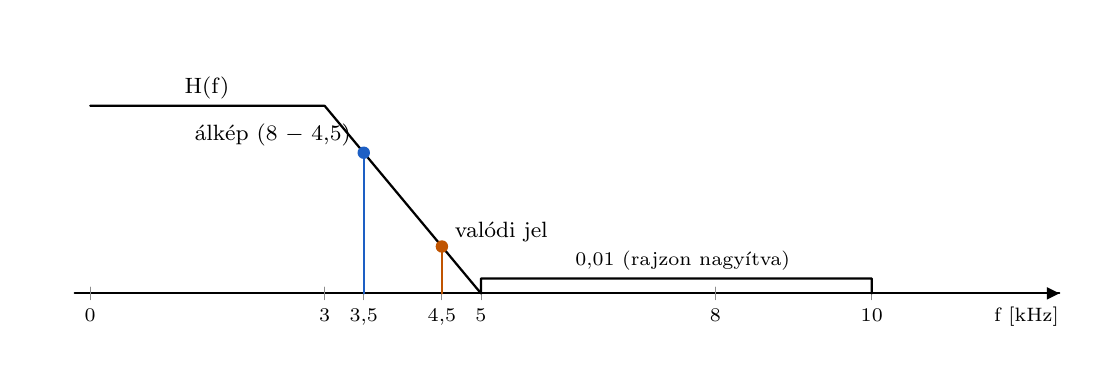
\begin{tikzpicture}[x=0.01985cm,y=-0.01985cm,line cap=round,line join=round]
\useasboundingbox (0,0) rectangle (680,210);
\path[draw=black,line width=0.7pt] (30,170) -- (660,170);
\path[fill=black,draw=none] (660,170) -- (652,166) -- (652,174) -- cycle;
\path[draw=black!45,line width=0.35pt] (40,166) -- (40,174);
\node[anchor=base,inner sep=0pt,font=\scriptsize] at (40,188) {0};
\path[draw=black!45,line width=0.35pt] (190,166) -- (190,174);
\node[anchor=base,inner sep=0pt,font=\scriptsize] at (190,188) {3};
\path[draw=black!45,line width=0.35pt] (215,166) -- (215,174);
\node[anchor=base,inner sep=0pt,font=\scriptsize] at (215,188) {3,5};
\path[draw=black!45,line width=0.35pt] (265,166) -- (265,174);
\node[anchor=base,inner sep=0pt,font=\scriptsize] at (265,188) {4,5};
\path[draw=black!45,line width=0.35pt] (290,166) -- (290,174);
\node[anchor=base,inner sep=0pt,font=\scriptsize] at (290,188) {5};
\path[draw=black!45,line width=0.35pt] (440,166) -- (440,174);
\node[anchor=base,inner sep=0pt,font=\scriptsize] at (440,188) {8};
\path[draw=black!45,line width=0.35pt] (540,166) -- (540,174);
\node[anchor=base,inner sep=0pt,font=\scriptsize] at (540,188) {10};
\node[anchor=base east,inner sep=0pt,font=\scriptsize] at (660,188) {f [kHz]};
\path[draw=black,line width=0.8pt] (40,50) -- (190,50) -- (290,170) -- (290,160.4) -- (540,160.4) -- (540,170);
\node[anchor=base west,inner sep=0pt,font=\footnotesize] at (100,42) {H(f)};
\node[anchor=base west,inner sep=0pt,font=\scriptsize] at (350,152.4) {0,01 (rajzon nagyítva)};
\path[draw=cB,line width=0.8pt] (265,170) -- (265,140);
\path[fill=cB,draw=none] (265,140) circle[radius=0.079cm];
\path[draw=cA,line width=0.8pt] (215,170) -- (215,80);
\path[fill=cA,draw=none] (215,80) circle[radius=0.079cm];
\node[anchor=base west,inner sep=0pt,font=\footnotesize] at (273,134) {valódi jel};
\node[anchor=base east,inner sep=0pt,font=\footnotesize] at (207,72) {álkép (8 $-$ 4,5)};
\end{tikzpicture}\end{center}


{\footnotesize\sffamily Forrás: TMIT gyak01 P.1.1 $\cdot$ Koma gyak2/2 $\cdot$ Marosi ik.4 $\cdot$ azonosítók: tg01\_P11, kg02\_2, mg2\_1. Címkék: beugró}
\end{feladat}
\begin{keresunk}
\begin{itemize}
\item a) a szivárgó komponensek frekvenciája és amplitúdója
\item b) a kimenő komponensek frekvenciája és amplitúdója
\end{itemize}
\end{keresunk}
\begin{jeloles}
\begin{jeltabla}
$\ca{f_s}$ & mintavételi frekvencia & $8$\,kHz\\
$\cb{T}$ & mintavételi idő & $125$\,\textmu{}s\\
$f$ & a bemenő jel frekvenciája & \\
$H$ & a szűrő átvitele & \\
$n$ & tetszőleges egész szám & \\
$f_\text{ki}$ & egy kimenő összetevő frekvenciája & \\
$f_\text{be}$ & a bemenő szinusz frekvenciája & \\
$U_7$ & a kimenő 7 kHz-es összetevő amplitúdója & \\
$U_9$ & a kimenő 9 kHz-es összetevő amplitúdója & \\
$U_{15}$ & a kimenő 15 kHz-es összetevő amplitúdója & \\
$U_{17}$ & a kimenő 17 kHz-es összetevő amplitúdója & \\
$U_\text{minta}$ & a mintavevőre jutó összetevő amplitúdója (a bemenő szűrő után) & \\
$U_{4{,}5}$ & a kimenő 4,5 kHz-es összetevő amplitúdója & \\
$U_{3{,}5}$ & a kimenő 3,5 kHz-es összetevő amplitúdója & \\
\end{jeltabla}
\par\smallskip\textbf{Adott még:}
\begin{itemize}
\item a) $2$ V, $1$ kHz
\item b) $2$ V, $4{,}5$ kHz
\end{itemize}
\end{jeloles}
\begin{elmelet}[Miért így? Egyszerűen]
\textbf{Miért elég a frekvenciákat egyenként végignézni?}\par Mert a lánc lineáris: minden szinuszos komponens külön utat jár be (bemenő szűrő $\to$ mintavétel $\to$ kimenő szűrő), és a végén összeadódnak.

\textbf{Miért pont $n f_s\pm f$ helyeken vannak a másolatok?}\par Mert a mintavétel a spektrumot $f_s$-enként eltolva megismétli, és a valós szinusznak $+f$ és $-f$ vonala is van. A $-f$ vonal $f_s$-sel eltolva adja az $f_s-f$ álképet.

\textbf{Miért nem a bemenő szűrő a hibás az a) részben?}\par Az $1$ kHz-et a bemenő szűrő változatlanul átengedi, ott nincs mit levágni. A $7$ és $9$ kHz-es komponens a D/A után keletkezik, és a kimenő szűrő engedi át gyengítve: ez \textbf{szivárgás}.

\textbf{Miért rosszabb a b) eset?}\par A $4{,}5$ kHz az $f_s/2=4$ kHz fölött van, ezért az $8-4{,}5=3{,}5$ kHz-es álképe a hasznos sávba esik, ahol a kimenő szűrő alig csillapít. Ez \textbf{aliasing}, és a végén az álkép erősebb lesz, mint a valódi jel.
\end{elmelet}
\begin{elmelet}[Felhasznált elmélet]
\textbf{Mintavett jel spektruma.} A minták spektruma az eredeti $f_s$-enként eltolt másolatainak összege (A2).
\begin{center}\adjustbox{max width=\linewidth}{$\displaystyle \hat X(f)=H_\text{ki}(f)\sum_i H_\text{be}(f-i f_s)\,X(f-i f_s)$}\end{center}


\textbf{Szűrők láncban.} Egy komponens kimeneti amplitúdója a bemenő amplitúdó és a két szűrő értékének szorzata, mindegyik a saját frekvenciáján (A4).
\end{elmelet}

\lepes{A mintasorozat spektruma}
Az $1$ kHz-es bemenet a bemenő szűrőn csillapítatlanul átjut, a mintavétel után $n\cdot 8\pm1$ kHz-en lesznek vonalai.

\begin{center}\adjustbox{max width=\linewidth}{$\displaystyle f_\text{ki}=n {\ca{f_s}}\pm f_\text{be}=n\cdot 8\pm 1\ \text{kHz}$}\end{center}
\jegyzet{definíció}{$n$ egész}

\begin{center}\adjustbox{max width=\linewidth}{$\displaystyle f_\text{ki}\in\{1;\ 7;\ 9;\ 15;\ 17;\ \ldots\}\ \text{kHz}$}\end{center}
\jegyzet{számérték}{$n\cdot8\pm1$, $n=0,1,2$}

\lepes{A kimenő szűrő hatása az a) esetben}
A kimenő szűrő $10$ kHz felett mindent levág, $5\ldots10$ kHz között $0{,}01$-szeresre csillapít.

\begin{center}\adjustbox{max width=\linewidth}{$\displaystyle U_7=2\,\text{V}\cdot H_\text{be}(1)\cdot H_\text{ki}(7)=2\cdot1\cdot0{,}01=0{,}02\ \text{V}$}\end{center}
\jegyzet{behelyettesítés}{ugyanígy $U_9=0{,}02$ V}

\begin{center}\adjustbox{max width=\linewidth}{$\displaystyle H_\text{ki}(15)=H_\text{ki}(17)=0\ \Longrightarrow\ U_{15}=U_{17}=0$}\end{center}
\jegyzet{ellenőrzés}{a 10 kHz feletti másolatok eltűnnek}

\lepes{A bemenő szűrő a b) esetben}
A $4{,}5$ kHz-es komponens a bemenő szűrő ferde szakaszára esik.

\begin{center}\adjustbox{max width=\linewidth}{$\displaystyle H_\text{be}(4{,}5)=2{,}5-\frac{4{,}5}{2}=0{,}25$}\end{center}
\jegyzet{behelyettesítés}{a ferde szakasz képlete, $f=4{,}5$}

\begin{center}\adjustbox{max width=\linewidth}{$\displaystyle U_\text{minta}=2\,\text{V}\cdot0{,}25=0{,}5\ \text{V}$}\end{center}
\jegyzet{számérték}{ennyi jut a mintavevőre}

\lepes{Az álkép és a valódi komponens a kimeneten}
A mintavétel után $n\cdot8\pm4{,}5$ kHz vonalak keletkeznek. A kimenő szűrő a $10$ kHz alattiakat engedi át: a $4{,}5$ és a $3{,}5$ kHz-est.

\begin{center}\adjustbox{max width=\linewidth}{$\displaystyle H_\text{ki}(4{,}5)=0{,}25\qquad H_\text{ki}(3{,}5)=2{,}5-\frac{3{,}5}{2}=0{,}75$}\end{center}
\jegyzet{behelyettesítés}{a kimenő szűrő ugyanaz a trapéz, $3{,}5=8-4{,}5$}

\begin{center}\adjustbox{max width=\linewidth}{$\displaystyle U_{4{,}5}=0{,}5\cdot0{,}25=0{,}125\ \text{V}\qquad U_{3{,}5}=0{,}5\cdot0{,}75=0{,}375\ \text{V}$}\end{center}
\jegyzet{számérték}{az álkép háromszor erősebb}

\begin{center}\adjustbox{max width=\linewidth}{$\displaystyle H_\text{ki}(8+4{,}5)=H_\text{ki}(12{,}5)=0$}\end{center}
\jegyzet{ellenőrzés}{a többi másolat nem jut át}
\begin{eredmeny}

\begin{center}\adjustbox{max width=\linewidth}{$\displaystyle \text{a) } 1\ \text{kHz: } 2\ \text{V}\qquad 7\ \text{és}\ 9\ \text{kHz: } 0{,}02\ \text{V (szivárgás)}$}\end{center}

\begin{center}\adjustbox{max width=\linewidth}{$\displaystyle \text{b) } 4{,}5\ \text{kHz: } 0{,}125\ \text{V}\qquad 3{,}5\ \text{kHz: } 0{,}375\ \text{V (aliasing)}$}\end{center}
\end{eredmeny}
\begin{tipp}[Ellenőrzés]
\begin{itemize}
\item Mértékegység: $H$ dimenzió nélküli, a kimenet V.
\item Határeset: ha $H_\text{be}(4{,}5)=0$ lenne, se jel, se álkép nem lenne. A szorzat ezt helyesen adja.
\item A Koma-jegyzet, a TMIT-füzet és Marosi táblai megoldása ugyanezt adja.
\end{itemize}
\end{tipp}
\begin{figyelem}[Tipikus hibák]
\begin{itemize}
\item Az álképet a bemenő szűrőn a $3{,}5$ kHz-en csillapítják ($0{,}75$), pedig ott még $4{,}5$ kHz a frekvencia ($0{,}25$).
\item Elfelejtik, hogy a valódi $4{,}5$ kHz-es komponens kétszer csillapodik (be és ki), ezért lesz csak $0{,}125$ V.
\end{itemize}
\end{figyelem}
\begin{tipp}[Saját számpélda (kiegészítés, a forrásban nem szerepel)]
\small
\begin{verbatim}
Ha a bemenet 4,2 kHz: H_be(4,2) = 0,4, álkép 3,8 kHz-en H_ki = 0,6.
Kimenet: 4,2 kHz 2*0,4*0,4 = 0,32 V, 3,8 kHz 2*0,4*0,6 = 0,48 V.
\end{verbatim}
\end{tipp}
\begin{tipp}[Kapcsolat és analógia]

\par\noindent{\small\renewcommand{\arraystretch}{1.25}\begin{tabularx}{\linewidth}{@{}>{\raggedright\arraybackslash}X>{\raggedright\arraybackslash}X@{}}\toprule
bemenő szűrő gyenge & aliasing, a hasznos sávban, utólag nem javítható\\
kimenő szűrő gyenge & szivárgás, a hasznos sávon kívül, jobb szűrővel javítható\\
\bottomrule\end{tabularx}}\par
\end{tipp}


% ------------------------------------------------------------------
\section{\texorpdfstring{2.2. feladat: PCM, 1,8 kHz, 40 dB-es szűrők: szivárgás és egyenirányítás}{2.2. feladat: PCM, 1,8 kHz, 40 dB-es szűrők: szivárgás és egyenirányítás}}\label{p2_02}
\setcounter{lepes}{0}
\begin{feladat}{2.2. feladat}
Egy $8$ kHz-es PCM rendszer bemenő és kimenő szűrője a zárótartományban ($4$ kHz felett) $40$ dB csillapítású, a $0{,}3\ldots3{,}4$ kHz sávban tökéletes. A bemenet $2$ V, $1{,}8$ kHz. a) Mekkora a kimenet $6{,}2$ kHz-es komponense? b) Milyen frekvenciák vannak még a kimeneten? c) Mi jelenhet meg, ha a bemenő jelet egyenirányítjuk?

{\footnotesize\sffamily Forrás: OneDrive 1-5 gyakorlatok 2.2 $\cdot$ Koma gyak2/1 $\cdot$ TMIT G.1.1 $\cdot$ azonosítók: pd02\_2, kg02\_1, tg01\_G11. Címkék: vizsga}
\end{feladat}
\begin{keresunk}
\begin{itemize}
\item a) $U_{6{,}2}$ (a kimenő 6,2 kHz-es összetevő amplitúdója)
\item b) a kimenő frekvenciák listája
\item c) az egyenirányított jel komponensei
\end{itemize}
\end{keresunk}
\begin{jeloles}
\begin{jeltabla}
$\ca{f_s}$ & mintavételi frekvencia & $8$\,kHz\\
$\cb{f}$ & a bemenő jel frekvenciája & $1{,}8$\,kHz\\
$\cc{U}$ & a bemenő jel amplitúdója & $2$\,V\\
$U_{6{,}2}$ & a kimenő 6,2 kHz-es összetevő amplitúdója & \emph{keresett}\\
$n$ & tetszőleges egész szám & \\
$f_\text{ki}$ & egy kimenő összetevő frekvenciája & \\
$f_0$ & az egyenirányított jel alapfrekvenciája & \\
$f_k$ & az egyenirányított jel k-adik felharmonikusának frekvenciája & \\
$k$ & a felharmonikus sorszáma (pozitív egész) & \\
\end{jeltabla}
\par\smallskip\textbf{Adott még:}
\begin{itemize}
\item zárótartomány: $40$ dB, azaz $\times0{,}01$ amplitúdóban
\end{itemize}
\end{jeloles}
\begin{elmelet}[Miért így? Egyszerűen]
\textbf{Miért $0{,}01$ a 40 dB?}\par Mert amplitúdóra $20\lg$ kell: $10^{-40/20}=0{,}01$. Teljesítményben ez $10^{-4}$.

\textbf{Miért csak a kimenő szűrő számít a $6{,}2$ kHz-nél?}\par Az $1{,}8$ kHz a bemenő szűrőn csillapítatlanul átjut. A $6{,}2$ kHz a mintavétel után keletkezik ($8-1{,}8$), ezért csak a kimenő szűrőn csillapodik.

\textbf{Miért veszélyes az egyenirányítás?}\par Az egyenirányított szinusz periodikus, de nem szinuszos: alapfrekvenciája $2\cdot1{,}8=3{,}6$ kHz, és sok felharmonikusa van. A $4$ kHz feletti felharmonikusok a bemenő szűrőn csak csillapodnak, és az álképeik a hasznos sávba eshetnek.
\end{elmelet}
\begin{elmelet}[Felhasznált elmélet]
\textbf{Álképek.} Egy $f$ frekvenciájú bemenet a mintavétel után az $n f_s\pm f$ frekvenciákon is megjelenik ($n$ egész).

\textbf{Decibel amplitúdóban.} Feszültség- (amplitúdó-) arányra $a_\mathrm{dB}=20\lg(U_1/U_2)$.
\begin{center}\adjustbox{max width=\linewidth}{$\displaystyle U_2=U_1\cdot10^{-a/20}$}\end{center}

\end{elmelet}

\lepes{A 6,2 kHz-es komponens}
Ez az ${\cb{1{,}8}}$ kHz álképe az első másolatnál, a kimenő szűrő zárótartományában.

\begin{center}\adjustbox{max width=\linewidth}{$\displaystyle {\cb{f}}={\ca{f_s}}-{\cb{1{,}8}}=8-{\cb{1{,}8}}=6{,}2\ \text{kHz}$}\end{center}
\jegyzet{definíció}{$n=1$, mínusz előjel}

\begin{center}\adjustbox{max width=\linewidth}{$\displaystyle U_{6{,}2}=2\,\text{V}\cdot10^{-40/20}=2\cdot0{,}01=0{,}02\ \text{V}$}\end{center}
\jegyzet{behelyettesítés}{20 mV}

\lepes{A többi kimenő komponens}
Minden másolat megjelenik, a kimenő szűrő mindet $0{,}01$-szeresre csillapítja.

\begin{center}\adjustbox{max width=\linewidth}{$\displaystyle f_\text{ki}=n\cdot8\pm{\cb{1{,}8}}\ \text{kHz}\ \Longrightarrow\ {\cb{1{,}8}};\ 6{,}2;\ 9{,}8;\ 14{,}2;\ 17{,}8;\ \ldots$}\end{center}
\jegyzet{definíció}{mind 20 mV, kivéve az 1,8 kHz-et (2 V)}

\lepes{Egyenirányítás}
A $|\sin|$ alakú jel alapfrekvenciája a kétszeres, és vannak felharmonikusai.

\begin{center}\adjustbox{max width=\linewidth}{$\displaystyle f_0=2\cdot{\cb{1{,}8}}=3{,}6\ \text{kHz}\qquad f_k=k\cdot3{,}6\ \text{kHz}$}\end{center}
\jegyzet{definíció}{az egyenirányított szinusz periódusa a fele}

\begin{center}\adjustbox{max width=\linewidth}{$\displaystyle f_\text{ki}=n\cdot8\pm k\cdot3{,}6\ \text{kHz}$}\end{center}
\jegyzet{átalakítás}{a mintavétel után}

\begin{center}\adjustbox{max width=\linewidth}{$\displaystyle n=1:\ 8-7{,}2=0{,}8\qquad 10{,}8-8=2{,}8\ \text{kHz}$}\end{center}
\jegyzet{számérték}{$k=2$: 7,2 kHz, $k=3$: 10,8 kHz}

\begin{center}\adjustbox{max width=\linewidth}{$\displaystyle n=2:\ 16-14{,}4=1{,}6\qquad 18-16=2{,}0\ \text{kHz}$}\end{center}
\jegyzet{számérték}{ezek is a 0,3\ldots{}3,4 kHz-es sávban vannak}
\begin{figyelem}[Javítás]
A források (OneDrive 2.2, Koma) példaként csak a $0{,}8$ és a $2{,}8$ kHz-et említik. A független ellenőrzés szerint a $2f_s$ körüli álképek közül az $1{,}6$ és a $2{,}0$ kHz is a hasznos sávba esik. Ez nem ellentmondás, csak kiegészítés.
\end{figyelem}
\begin{eredmeny}

\begin{center}\adjustbox{max width=\linewidth}{$\displaystyle U_{6{,}2}=20\ \text{mV}$}\end{center}

\begin{center}\adjustbox{max width=\linewidth}{$\displaystyle f_\text{ki}=n\cdot8\pm1{,}8\ \text{kHz}$}\end{center}

\begin{center}\adjustbox{max width=\linewidth}{$\displaystyle \text{egyenirányítva a hasznos sávban: } 0{,}8;\ 1{,}6;\ 2{,}0;\ 2{,}8\ \text{kHz}$}\end{center}
\end{eredmeny}
\begin{tipp}[Ellenőrzés]
\begin{itemize}
\item Az álképek nem harmonikusai az $1{,}8$ kHz-nek: ez hallható, „fals” torzítás.
\item A felharmonikus amplitúdója a bemenő szűrőn $40$ dB-t csillapodik, mégis megjelenik. Ez mutatja, hogy a 40 dB nem végtelen.
\end{itemize}
\end{tipp}
\begin{figyelem}[Tipikus hibák]
\begin{itemize}
\item $10\lg$-gel számolnak amplitúdóra, és $10^{-4}$-et kapnak $0{,}01$ helyett.
\item Az egyenirányított jelnél $1{,}8$ kHz-es alapharmonikussal számolnak. Az alapfrekvencia kétszeres lesz.
\end{itemize}
\end{figyelem}
\begin{tipp}[Saját számpélda (kiegészítés, a forrásban nem szerepel)]
\small
\begin{verbatim}
30 dB-es zárótartomány esetén: U(6,2 kHz) = 2*10^(-30/20) = 2*0,0316 = 63 mV.
\end{verbatim}
\end{tipp}
\begin{tipp}[Kapcsolat és analógia]

\par\noindent{\small\renewcommand{\arraystretch}{1.25}\begin{tabularx}{\linewidth}{@{}>{\raggedright\arraybackslash}X>{\raggedright\arraybackslash}X@{}}\toprule
túlvezérlés (2.12) & a vágás páratlan felharmonikusokat ad, az egyenirányítás párosakat\\
\bottomrule\end{tabularx}}\par
\end{tipp}


% ------------------------------------------------------------------
\section{\texorpdfstring{2.3. feladat: Két sávban lévő jel: teljesítménysűrűség és a mintavételi frekvencia}{2.3. feladat: Két sávban lévő jel: teljesítménysűrűség és a mintavételi frekvencia}}\label{p2_03}
\setcounter{lepes}{0}
\begin{feladat}{2.3. feladat}
Egy $50\ \Omega$-os ellenálláson mért feszültség spektrális sűrűsége a pozitív frekvenciákon zérus, kivéve a $0\ldots3$ kHz és a $7\ldots8$ kHz sávot, ahol állandó. A jel teljesítménye $0{,}2$ mW. a) Hogyan viselkedik a spektrális sűrűség a negatív frekvenciákon? b) Mekkora a spektrális sűrűség? c) Milyen $f_s$ mellett állítható vissza a jel, és milyen szűrővel?

{\footnotesize\sffamily Forrás: OneDrive 2.1 $\cdot$ TMIT P.1.2 $\cdot$ Koma gyak2/3 $\cdot$ Marosi ik.5 $\cdot$ azonosítók: pd02\_1, tg01\_P12, kg02\_3, mg2\_2. Címkék: beugró}
\end{feladat}
\begin{keresunk}
\begin{itemize}
\item a) a spektrum szimmetriája
\item b) $s_0$ teljesítmény- és feszültségnégyzet-sűrűségként
\item c) a megengedett $f_s$ (mintavételi frekvencia) tartományok és a szűrők
\end{itemize}
\end{keresunk}
\begin{jeloles}
\begin{jeltabla}
$B_\text{össz}$ & a jel teljes sávszélessége a pozitív frekvenciákon & \\
$\ca{P}$ & a jel teljesítménye & $0{,}2$\,mW\\
$\cb{R}$ & az ellenállás & $50$\\
$s_0$ & a jel teljesítménysűrűség-spektruma, s(f) & \emph{keresett}\\
$f_s$ & mintavételi frekvencia & \emph{keresett}\\
$f_{\max}$ & a jel legnagyobb frekvenciája (8 kHz) & \\
$s$ & a jel teljesítménysűrűség-spektruma, s(f) & \\
$f$ & frekvencia (a spektrum változója) & \\
\end{jeltabla}
\end{jeloles}
\begin{elmelet}[Miért így? Egyszerűen]
\textbf{Miért páros a spektrális sűrűség?}\par Mert a jel valós. A kétoldalas spektrumban minden szinuszos komponens fele $+f$-en, fele $-f$-en van.

\textbf{Miért $2\cdot4$ kHz a szélesség az integrálban?}\par Mert a kétoldalas sűrűséget a pozitív és a negatív frekvenciákon is integrálni kell.

\textbf{Miért lehet $16$ kHz alatt is mintavételezni?}\par A $3\ldots7$ kHz között üres hely van. Ha a $7\ldots8$ kHz-es sáv álképe pont ebbe esik, nem lapolódik rá semmire.
\end{elmelet}
\begin{elmelet}[Felhasznált elmélet]
\textbf{Parseval.} A teljesítmény a spektrális sűrűség teljes integrálja.
\begin{center}\adjustbox{max width=\linewidth}{$\displaystyle P=\int_{-\infty}^{\infty}s(f)\,\mathrm df$}\end{center}


\textbf{Feszültségből teljesítmény.} $P=U^2/R$, ezért a feszültségnégyzet-sűrűség $R$-szeres.
\end{elmelet}

\lepes{A sűrűség értéke}
A kétoldalas sűrűség $2\cdot4$ kHz szélességben állandó.

\begin{center}\adjustbox{max width=\linewidth}{$\displaystyle {\ca{P}}=s_0\cdot2B_\text{össz}$}\end{center}
\jegyzet{tétel}{Parseval}

\begin{center}\adjustbox{max width=\linewidth}{$\displaystyle s_0=\frac{P}{2B_\text{össz}}=\frac{0{,}2\ \text{mW}}{8\ \text{kHz}}=25\ \frac{\mu\text{W}}{\text{kHz}}$}\end{center}
\jegyzet{átalakítás}{$P=0{,}2$ mW, $2B_\text{össz}=8$ kHz}

\begin{center}\adjustbox{max width=\linewidth}{$\displaystyle s_0'={\cb{R}}\cdot s_0={\cb{50}}\cdot25\cdot10^{-9}\ \frac{\text{V}^2}{\text{Hz}}=1{,}25\cdot10^{-6}\ \frac{\text{V}^2}{\text{Hz}}=1250\ \frac{\text{mV}^2}{\text{kHz}}$}\end{center}
\jegyzet{átalakítás}{feszültségnégyzet-sűrűség}

\lepes{Aluláteresztő visszaállítás}
A legmagasabb frekvencia $8$ kHz.

\begin{center}\adjustbox{max width=\linewidth}{$\displaystyle f_s\ge2f_{\max}=16\ \text{kHz}$}\end{center}
\jegyzet{tétel}{aluláteresztő, határfrekvenciája 8 kHz és $f_s/2$ között}

\lepes{Kisebb mintavételi frekvencia}
A $7\ldots8$ kHz-es sáv negatív oldali másolatát ($-8\ldots-7$) $f_s$-sel eltolva a $3\ldots7$ kHz-es résbe kell tenni, és a $-3\ldots3$ kHz-es sáv másolata ($f_s-3\ldots f_s+3$) nem lóghat a $7\ldots8$ kHz-es sávba.

\begin{center}\adjustbox{max width=\linewidth}{$\displaystyle f_s-8\ge3\ \Longrightarrow\ f_s\ge11\ \text{kHz}$}\end{center}
\jegyzet{geometria}{a 7\ldots{}8 kHz álképe a 3 kHz felett}

\begin{center}\adjustbox{max width=\linewidth}{$\displaystyle f_s-7\le7\ \Longrightarrow\ f_s\le14\ \text{kHz}$}\end{center}
\jegyzet{geometria}{és a 7 kHz alatt marad}

\begin{center}\adjustbox{max width=\linewidth}{$\displaystyle f_s-3\ge8\ \Longleftarrow\ f_s\ge11$}\end{center}
\jegyzet{ellenőrzés}{az alapsáv másolata a 8 kHz felett van}
\begin{eredmeny}

\begin{center}\adjustbox{max width=\linewidth}{$\displaystyle s(-f)=s(f)\qquad s_0=25\ \tfrac{\mu\text{W}}{\text{kHz}}=1250\ \tfrac{\text{mV}^2}{\text{kHz}}$}\end{center}

\begin{center}\adjustbox{max width=\linewidth}{$\displaystyle f_s\ge16\ \text{kHz (aluláteresztő)}\qquad 11\le f_s\le14\ \text{kHz (két áteresztősávú szűrő)}$}\end{center}
\end{eredmeny}
\begin{tipp}[Ellenőrzés]
\begin{itemize}
\item $f_s=12$ kHz: álképek $4\ldots5$ kHz-en (a résben) és $9\ldots15$ kHz-en (a sáv felett). Jó.
\item $f_s=15$ kHz: a $7\ldots8$ álképe $7\ldots8$ kHz-re esne, rá a jelre. Rossz.
\end{itemize}
\end{tipp}
\begin{figyelem}[Tipikus hibák]
\begin{itemize}
\item Egyoldalas szélességgel ($4$ kHz) osztanak, és kétszeres $s_0$-t kapnak.
\item A $11\ldots14$ kHz-es tartománynál elfelejtik, hogy a visszaállításhoz nem aluláteresztő, hanem a két sávot kiválogató szűrő kell.
\end{itemize}
\end{figyelem}
\begin{tipp}[Saját számpélda (kiegészítés, a forrásban nem szerepel)]
\small
\begin{verbatim}
P = 0,5 mW esetén: s0 = 0,5 mW / 8 kHz = 62,5 uW/kHz, x50 Ohm = 3125 mV^2/kHz.
\end{verbatim}
\end{tipp}


% ------------------------------------------------------------------
\section{\texorpdfstring{2.4. feladat: Sáváteresztő mintavétel: 45\ldots{}75 kHz}{2.4. feladat: Sáváteresztő mintavétel: 45…75 kHz}}\label{p2_04}
\setcounter{lepes}{0}
\begin{feladat}{2.4. feladat}
Egy jelnek $45$ és $75$ kHz között vannak komponensei. a) Mekkora legyen $f_s$, ha aluláteresztő szűrővel állítjuk vissza? b) Sáváteresztő szűrő esetén mekkora lehet? c) Mekkora a legkisebb $f_s$?

{\footnotesize\sffamily Forrás: Vizsga 2016.01.05 1. $\cdot$ régi jegyzet F12 és M1-T012 $\cdot$ azonosítók: vz2016\_01\_05\_Q1, F12. Címkék: vizsga, beugró}
\end{feladat}
\begin{keresunk}
\begin{itemize}
\item a) $f_s$ (mintavételi frekvencia) aluláteresztővel
\item b) a sáváteresztő tartományok
\item c) a legkisebb $f_s$ (mintavételi frekvencia)
\end{itemize}
\end{keresunk}
\begin{jeloles}
\begin{jeltabla}
$\ca{f_L}$ & a jel legkisebb frekvenciája & $45$\,kHz\\
$\cb{f_H}$ & a jel legnagyobb frekvenciája & $75$\,kHz\\
$\cc{B}$ & a jel sávszélessége & $30$\,kHz\\
$f_s$ & mintavételi frekvencia & \emph{keresett}\\
$k$ & a Nyquist-zóna sorszáma: a frekvenciatengelyt $f_s/2$ széles sávokra osztjuk, és $k$ annak a sávnak a sorszáma, amelybe a jel teljes sávja beleesik & \\
$k_{\max}$ & a legnagyobb szóba jöhető zónasorszám, $\lfloor f_H/B\rfloor$ & \\
$f_{s,\min}$ & a legkisebb mintavételi frekvencia & \\
\end{jeltabla}
\end{jeloles}
\begin{elmelet}[Miért így? Egyszerűen]
\textbf{Miért van értelme a sáváteresztő mintavételnek?}\par A jel csak $30$ kHz széles, de magasan van. Ha a másolatok a sávok közé esnek, $150$ kHz helyett már $75$ kHz is elég.

\textbf{Meddig kell $k$-t növelni?}\par $k\le\lfloor f_H/B\rfloor=\lfloor75/30\rfloor=2$. Nagyobb $k$-ra az alsó határ meghaladná a felsőt.
\end{elmelet}
\begin{elmelet}[Felhasznált elmélet]
\textbf{Sáváteresztő mintavétel.} Ha a jel csak $f_L$ és $f_H$ között van ($B=f_H-f_L$), a megengedett mintavételi frekvenciák egész $k$-ra, $1\le k\le\lfloor f_H/B\rfloor$:
\begin{center}\adjustbox{max width=\linewidth}{$\displaystyle \frac{2f_H}{k}\le f_s\le\frac{2f_L}{k-1}$}\end{center}

\end{elmelet}

\lepes{Mit jelent a $k$? A Nyquist-zóna sorszáma}
A mintavétel után a spektrum $f_s$-enként ismétlődik. Osszuk fel a frekvenciatengelyt $f_s/2$ széles sávokra (Nyquist-zónákra): $0\ldots f_s/2$ az első, $f_s/2\ldots f_s$ a második, és így tovább. \textbf{$k$ annak a zónának a sorszáma, amelybe a jel teljes sávja beleesik:} $(k-1)\,f_s/2\le {\ca{f_L}}$ és ${\cb{f_H}}\le k\,f_s/2$. A két egyenlőtlenséget $f_s$-re rendezve kapjuk a megengedett tartományt, $2{\cb{f_H}}/k\le f_s\le2{\ca{f_L}}/(k-1)$. A $k=1$ eset a szokásos aluláteresztő mintavétel ($f_s\ge2{\cb{f_H}}$). Mivel a zóna nem lehet keskenyebb a jelnél ($f_s/2\ge {\cc{B}}$), $k$ legfeljebb ${\cb{f_H}}/{\cc{B}}$ lehet, lefelé kerekítve: $k_{\max}=\lfloor {\cb{f_H}}/{\cc{B}}\rfloor$.

\lepes{Aluláteresztő eset}
A legmagasabb komponens dönt.

\begin{center}\adjustbox{max width=\linewidth}{$\displaystyle f_s\ge2{\cb{f_H}}=2\cdot{\cb{75}}=150\ \text{kHz}$}\end{center}
\jegyzet{tétel}{$k=1$}

\lepes{A második Nyquist-zóna ($k=2$)}
Behelyettesítünk a sáváteresztő képletbe.
\behely{\bh{\ca{f_L}}{\ca{45\un{kHz}}} \bh{\cb{f_H}}{\cb{75\un{kHz}}}}

\begin{center}\adjustbox{max width=\linewidth}{$\displaystyle \frac{2\cdot{\cb{75}}}{2}\le f_s\le\frac{2\cdot{\ca{45}}}{1}$}\end{center}
\jegyzet{behelyettesítés}{$k=2$, $f_H=75$, $f_L=45$ kHz}

\begin{center}\adjustbox{max width=\linewidth}{$\displaystyle {\cb{75}}\ \text{kHz}\le f_s\le90\ \text{kHz}$}\end{center}
\jegyzet{számérték}{kiszámolva}

\lepes{Ellenőrzés a spektrumon}
$f_s={\cb{75}}$ kHz-nél a negatív oldali sáv ($-{\cb{75}}\ldots-{\ca{45}}$) eltolva $0\ldots{\cc{30}}$ kHz-re kerül, $2f_s$-sel ${\cb{75}}\ldots105$ kHz-re. Egyik sem lóg bele a ${\ca{45}}\ldots{\cb{75}}$ kHz-be.

\begin{center}\adjustbox{max width=\linewidth}{$\displaystyle f_s={\cb{75}}:\ \ [0;{\cc{30}}]\ \text{és}\ [{\cb{75}};105]\ \cap\ [{\ca{45}};{\cb{75}}]=\{75\}$}\end{center}
\jegyzet{ellenőrzés}{csak a sávszél érintkezik, ezért határeset}
\begin{eredmeny}

\begin{center}\adjustbox{max width=\linewidth}{$\displaystyle \text{a) } f_s\ge150\ \text{kHz}\qquad\text{b) } 75\le f_s\le90\ \text{kHz}\qquad\text{c) } f_{s,\min}=75\ \text{kHz}$}\end{center}
\end{eredmeny}
\begin{tipp}[Ellenőrzés]
\begin{itemize}
\item $f_s\ge2B=60$ kHz minden megoldásra teljesül.
\item A vizsgamegoldás ugyanezt adja az $f_s-45\le45$ és $2f_s-75\ge75$ feltételekből.
\end{itemize}
\end{tipp}
\begin{figyelem}[Tipikus hibák]
\begin{itemize}
\item $2B=60$ kHz-et mondanak legkisebbnek. Az csak akkor jó, ha $f_H/B$ egész, itt $2{,}5$.
\item Sáváteresztő mintavételnél aluláteresztő visszaállító szűrőt rajzolnak.
\end{itemize}
\end{figyelem}
\begin{tipp}[Saját számpélda (kiegészítés, a forrásban nem szerepel)]
\small
\begin{verbatim}
60...80 kHz (B = 20): k = 4 -> csak 40 kHz, k = 3 -> 53,3...60 kHz, k = 2 ->
  80...120 kHz.
\end{verbatim}
\end{tipp}


% ------------------------------------------------------------------
\section{\texorpdfstring{2.5. feladat: 40\ldots{}70 kHz, gyök 2-es csúcstényező, 64 dB}{2.5. feladat: 40…70 kHz, gyök 2-es csúcstényező, 64 dB}}\label{p2_05}
\setcounter{lepes}{0}
\begin{feladat}{2.5. feladat}
Tervezzen mintavevő rendszert egyenletes kvantálóval, amely egy valós, $\sqrt2$ csúcstényezőjű, teljes kivezérlésű jel visszaállításakor legalább $64$ dB-es jel-zaj viszonyt ad. A jel $40$ és $70$ kHz között tartalmaz komponenseket. a) Mik az átlapolódásmentes mintavételi frekvenciák? b) Milyen szűrők kellenek? c) Hány bites kvantáló kell, ha aluláteresztő szűrőkkel állítjuk vissza?

{\footnotesize\sffamily Forrás: Moodle-vizsga 2020.06.02 Q8 (3/3 pont) $\cdot$ F14 $\cdot$ azonosító: vz2020\_06\_02\_Q8. Címkék: vizsga}
\end{feladat}
\begin{keresunk}
\begin{itemize}
\item a) $f_s$ (mintavételi frekvencia) tartományok
\item b) a szűrők típusa
\item c) $n$ (a kvantáló bitszáma)
\end{itemize}
\end{keresunk}
\begin{jeloles}
\begin{jeltabla}
$\ca{f_L}$ & a jel legkisebb frekvenciája & $40$\\
$\cb{f_H}$ & a jel legnagyobb frekvenciája & $70$\,kHz\\
$\cc{B}$ & a jel sávszélessége & $30$\,kHz\\
$C$ & csúcstényező & \\
$f_s$ & mintavételi frekvencia & \emph{keresett}\\
$n$ & a kvantáló bitszáma & \emph{keresett}\\
$k$ & a Nyquist-zóna sorszáma: a frekvenciatengelyt $f_s/2$ széles sávokra osztjuk, és $k$ annak a sávnak a sorszáma, amelybe a jel teljes sávja beleesik & \\
$k_{\max}$ & a legnagyobb szóba jöhető zónasorszám, $\lfloor f_H/B\rfloor$ & \\
\end{jeltabla}
\end{jeloles}
\begin{elmelet}[Miért így? Egyszerűen]
\textbf{Miért $f_s=2B$ a c) részben?}\par Aluláteresztő visszaállításnál a szűrő sávja $B=70$ kHz, és a legkisebb $f_s=140$ kHz. Ekkor $f_s/2B=1$, a túlmintavételezés nem ad nyereséget.

\textbf{Miért felfelé kerekítünk?}\par Mert a $64$ dB alsó korlát. $10$ bittel $62$ dB lenne, az kevés.
\end{elmelet}
\begin{elmelet}[Felhasznált elmélet]
\textbf{Sáváteresztő mintavétel.} Ha a jel csak $f_L$ és $f_H$ között van ($B=f_H-f_L$), a megengedett mintavételi frekvenciák egész $k$-ra, $1\le k\le\lfloor f_H/B\rfloor$:
\begin{center}\adjustbox{max width=\linewidth}{$\displaystyle \frac{2f_H}{k}\le f_s\le\frac{2f_L}{k-1}$}\end{center}


\textbf{Jel-zaj viszony.} Egyenletes kvantálásnál, $C$ csúcstényezőjű, teljes kivezérlésű jelre, $n$ bittel, $B$ sávú visszaállító szűrővel:
\begin{center}\adjustbox{max width=\linewidth}{$\displaystyle \text{SNR}_{\mathrm{dB}}=10\lg\frac{3}{C^2}+10\lg\frac{f_s}{2B}+6{,}02\,n$}\end{center}

\end{elmelet}

\lepes{Mit jelent a $k$? A Nyquist-zóna sorszáma}
A mintavétel után a spektrum $f_s$-enként ismétlődik. Osszuk fel a frekvenciatengelyt $f_s/2$ széles sávokra (Nyquist-zónákra): $0\ldots f_s/2$ az első, $f_s/2\ldots f_s$ a második, és így tovább. \textbf{$k$ annak a zónának a sorszáma, amelybe a jel teljes sávja beleesik:} $(k-1)\,f_s/2\le {\ca{f_L}}$ és ${\cb{f_H}}\le k\,f_s/2$. A két egyenlőtlenséget $f_s$-re rendezve kapjuk a megengedett tartományt, $2{\cb{f_H}}/k\le f_s\le2{\ca{f_L}}/(k-1)$. A $k=1$ eset a szokásos aluláteresztő mintavétel ($f_s\ge2{\cb{f_H}}$). Mivel a zóna nem lehet keskenyebb a jelnél ($f_s/2\ge {\cc{B}}$), $k$ legfeljebb ${\cb{f_H}}/{\cc{B}}$ lehet, lefelé kerekítve: $k_{\max}=\lfloor {\cb{f_H}}/{\cc{B}}\rfloor$.

\lepes{Mintavételi tartományok}
$\lfloor{\cb{70}}/{\cc{30}}\rfloor=2$, tehát $k=1$ és $k=2$.

\begin{center}\adjustbox{max width=\linewidth}{$\displaystyle k=1:\ f_s\ge140\ \text{kHz}$}\end{center}
\jegyzet{tétel}{$2f_H=2\cdot70$}
\behely{\bh{\cb{f_H}}{\cb{70\un{kHz}}}}

\begin{center}\adjustbox{max width=\linewidth}{$\displaystyle k=2:\ \frac{140}{2}\le f_s\le\frac{80}{1}\ \Longrightarrow\ {\cb{70}}\le f_s\le80\ \text{kHz}$}\end{center}
\jegyzet{behelyettesítés}{$2f_H/2$ és $2f_L/1$}

\lepes{A szűrők}
A $140$ kHz feletti esetben a be- és kimenő szűrő aluláteresztő, a ${\cb{70}}\ldots80$ kHz-es esetben sáváteresztő (${\ca{40}}\ldots{\cb{70}}$ kHz).

\lepes{A bitszám}
Szinuszra $10\lg(3/2)=1{,}76$ dB, és $f_s/2{\cc{B}}=1$.

\begin{center}\adjustbox{max width=\linewidth}{$\displaystyle 1{,}76+0+6{,}02\,n\ge64$}\end{center}
\jegyzet{behelyettesítés}{aluláteresztő visszaállítás: $10\lg(f_s/2B)=0$}

\begin{center}\adjustbox{max width=\linewidth}{$\displaystyle n\ge\frac{64-1{,}76}{6{,}02}=10{,}34$}\end{center}
\jegyzet{átalakítás}{$n$-re rendezve}

\begin{center}\adjustbox{max width=\linewidth}{$\displaystyle n=11\ \text{bit}$}\end{center}
\jegyzet{számérték}{felfelé kerekítve}
\begin{eredmeny}

\begin{center}\adjustbox{max width=\linewidth}{$\displaystyle f_s\ge140\ \text{kHz (aluláteresztő)}\qquad 70\le f_s\le80\ \text{kHz (sáváteresztő)}\qquad n=11\ \text{bit}$}\end{center}
\end{eredmeny}
\begin{tipp}[Ellenőrzés]
\begin{itemize}
\item $n=11$: $1{,}76+66{,}2=68{,}0$ dB $\ge64$ dB. $n=10$: $62{,}0$ dB, kevés.
\item A javító 1+1+1 pontot adott erre a megoldásra.
\end{itemize}
\end{tipp}
\begin{figyelem}[Tipikus hibák]
\begin{itemize}
\item $6n\ge64$-ből $n=11$ jön ki, de az $1{,}76$ dB elhagyása szerencsés esetben ugyanazt adja, máskor nem. Írd fel a teljes képletet.
\end{itemize}
\end{figyelem}
\begin{tipp}[Saját számpélda (kiegészítés, a forrásban nem szerepel)]
\small
\begin{verbatim}
Ha 80 dB kell: n >= (80 - 1,76)/6,02 = 13,0 -> 13 bit (13*6,02 + 1,76 = 80,0 dB,
  épp elég).
\end{verbatim}
\end{tipp}


% ------------------------------------------------------------------
\section{\texorpdfstring{2.6. feladat: 60\ldots{}108 kHz, háromszögjel, 70 dB}{2.6. feladat: 60…108 kHz, háromszögjel, 70 dB}}\label{p2_06}
\setcounter{lepes}{0}
\begin{feladat}{2.6. feladat}
Egyenletes kvantálót kell tervezni, amely egy $\sqrt3$ csúcstényezőjű (háromszög alakú), teljes kivezérlésű jel visszaállításakor legalább $70$ dB-es jel-zaj viszonyt ad. A jel $60$ és $108$ kHz között tartalmaz komponenseket. a) Mik a választható mintavételi frekvenciák? b) Hány bites kvantáló kell?

{\footnotesize\sffamily Forrás: Hallgatói vizsgamegoldás 2014.12.15/4 és 2014.01.14/2 $\cdot$ azonosító: vz2014\_12\_15\_Q4. Címkék: vizsga}
\end{feladat}
\begin{keresunk}
\begin{itemize}
\item a) $f_s$ (mintavételi frekvencia) tartományok
\item b) $n$ (a kvantáló bitszáma)
\end{itemize}
\end{keresunk}
\begin{jeloles}
\begin{jeltabla}
$\ca{f_L}$ & a jel legkisebb frekvenciája & $60$\\
$\cb{f_H}$ & a jel legnagyobb frekvenciája & $108$\,kHz\\
$\cc{B}$ & a jel sávszélessége & $48$\,kHz\\
$C$ & csúcstényező & \\
$f_s$ & mintavételi frekvencia & \emph{keresett}\\
$n$ & a kvantáló bitszáma & \emph{keresett}\\
$k$ & a Nyquist-zóna sorszáma: a frekvenciatengelyt $f_s/2$ széles sávokra osztjuk, és $k$ annak a sávnak a sorszáma, amelybe a jel teljes sávja beleesik & \\
$k_{\max}$ & a legnagyobb szóba jöhető zónasorszám, $\lfloor f_H/B\rfloor$ & \\
\end{jeltabla}
\end{jeloles}
\begin{elmelet}[Miért így? Egyszerűen]
\textbf{Miért pont a háromszögjel kényelmes?}\par Mert $3/C^2=1$, így a konstans tag eltűnik, és $\text{SNR}_{\mathrm{dB}}\approx6{,}02\,n$.

\textbf{Miért $f_s=2B$-vel számolunk a bitszámnál?}\par A forrásmegoldás ezt a legkisebb, „célszerűen választott” mintavételt veszi. Nagyobb $f_s$-nél kevesebb bit is elég lehet (A6).
\end{elmelet}
\begin{elmelet}[Felhasznált elmélet]
\textbf{Sáváteresztő mintavétel.} Ha a jel csak $f_L$ és $f_H$ között van ($B=f_H-f_L$), a megengedett mintavételi frekvenciák egész $k$-ra, $1\le k\le\lfloor f_H/B\rfloor$:
\begin{center}\adjustbox{max width=\linewidth}{$\displaystyle \frac{2f_H}{k}\le f_s\le\frac{2f_L}{k-1}$}\end{center}


\textbf{Jel-zaj viszony.} Egyenletes kvantálásnál, $C$ csúcstényezőjű, teljes kivezérlésű jelre, $n$ bittel, $B$ sávú visszaállító szűrővel:
\begin{center}\adjustbox{max width=\linewidth}{$\displaystyle \text{SNR}_{\mathrm{dB}}=10\lg\frac{3}{C^2}+10\lg\frac{f_s}{2B}+6{,}02\,n$}\end{center}

\end{elmelet}

\lepes{Mit jelent a $k$? A Nyquist-zóna sorszáma}
A mintavétel után a spektrum $f_s$-enként ismétlődik. Osszuk fel a frekvenciatengelyt $f_s/2$ széles sávokra (Nyquist-zónákra): $0\ldots f_s/2$ az első, $f_s/2\ldots f_s$ a második, és így tovább. \textbf{$k$ annak a zónának a sorszáma, amelybe a jel teljes sávja beleesik:} $(k-1)\,f_s/2\le {\ca{f_L}}$ és ${\cb{f_H}}\le k\,f_s/2$. A két egyenlőtlenséget $f_s$-re rendezve kapjuk a megengedett tartományt, $2{\cb{f_H}}/k\le f_s\le2{\ca{f_L}}/(k-1)$. A $k=1$ eset a szokásos aluláteresztő mintavétel ($f_s\ge2{\cb{f_H}}$). Mivel a zóna nem lehet keskenyebb a jelnél ($f_s/2\ge {\cc{B}}$), $k$ legfeljebb ${\cb{f_H}}/{\cc{B}}$ lehet, lefelé kerekítve: $k_{\max}=\lfloor {\cb{f_H}}/{\cc{B}}\rfloor$.

\lepes{Mintavételi tartományok}
$\lfloor{\cb{108}}/{\cc{48}}\rfloor=2$.

\begin{center}\adjustbox{max width=\linewidth}{$\displaystyle k=1:\ f_s\ge216\ \text{kHz}$}\end{center}
\jegyzet{tétel}{$2f_H=2\cdot108$}
\behely{\bh{\cb{f_H}}{\cb{108\un{kHz}}}}

\begin{center}\adjustbox{max width=\linewidth}{$\displaystyle k=2:\ \frac{216}{2}\le f_s\le\frac{120}{1}\ \Longrightarrow\ {\cb{108}}\le f_s\le120\ \text{kHz}$}\end{center}
\jegyzet{behelyettesítés}{$2f_H/2$ és $2f_L/1=2\cdot60$}

\begin{center}\adjustbox{max width=\linewidth}{$\displaystyle f_s\ge2{\cc{B}}=96\ \text{kHz}$}\end{center}
\jegyzet{ellenőrzés}{teljesül}

\lepes{A bitszám}
$10\lg(3/C^2)=10\lg1=0$ dB.

\begin{center}\adjustbox{max width=\linewidth}{$\displaystyle 0+6{,}02\,n\ge70$}\end{center}
\jegyzet{behelyettesítés}{túlmintavételezési nyereség nélkül}

\begin{center}\adjustbox{max width=\linewidth}{$\displaystyle n\ge\frac{70}{6{,}02}=11{,}63$}\end{center}
\jegyzet{átalakítás}{$n$-re rendezve}

\begin{center}\adjustbox{max width=\linewidth}{$\displaystyle n=12\ \text{bit}$}\end{center}
\jegyzet{számérték}{felfelé kerekítve}
\begin{eredmeny}

\begin{center}\adjustbox{max width=\linewidth}{$\displaystyle f_s\ge216\ \text{kHz}\quad\text{vagy}\quad108\le f_s\le120\ \text{kHz}\qquad n=12\ \text{bit}$}\end{center}
\end{eredmeny}
\begin{tipp}[Ellenőrzés]
\begin{itemize}
\item $n=12$: $72{,}2$ dB $\ge70$. $n=11$: $66{,}2$ dB, kevés.
\item A középfrekvenciás alak ($f_c=84$ kHz, $(2f_c\mp B)/(m)$) ugyanezt a $108\ldots120$ kHz-es tartományt adja.
\end{itemize}
\end{tipp}
\begin{figyelem}[Tipikus hibák]
\begin{itemize}
\item $\sqrt3$ helyett $\sqrt2$-vel számolnak, és $1{,}76$ dB-t adnak hozzá. Ez itt egy bitet is jelenthet.
\end{itemize}
\end{figyelem}
\begin{tipp}[Saját számpélda (kiegészítés, a forrásban nem szerepel)]
\small
\begin{verbatim}
Ha f_s = 216 kHz, de a visszaállító szűrő csak a 60...108 kHz-et engedi át
  (sáváteresztő): f_s/2B = 216/96 = 2,25 -> +3,5 dB, n >= 66,5/6,02 = 11,05 -> 12
  bit (épp nem lesz elég a 11).
\end{verbatim}
\end{tipp}


% ------------------------------------------------------------------
\section{\texorpdfstring{2.7. feladat: Négyszögjel: a kimeneten 1, 3, 7 és 9 kHz}{2.7. feladat: Négyszögjel: a kimeneten 1, 3, 7 és 9 kHz}}\label{p2_07}
\setcounter{lepes}{0}
\begin{feladat}{2.7. feladat}
A láncban ideális aluláteresztő bemenő ($f_{AA}$) és visszaállító ($f_R$) szűrő van, a sávszélességük nem egyezik. A bemenetre $1$ kHz-es szimmetrikus négyszögjelet adunk. A kimeneten csak $1$, $3$, $7$ és $9$ kHz-es komponensek jelennek meg. a) Mekkora lehet a két szűrő sávszélessége? b) Mekkora a mintavételi frekvencia?
\begin{center}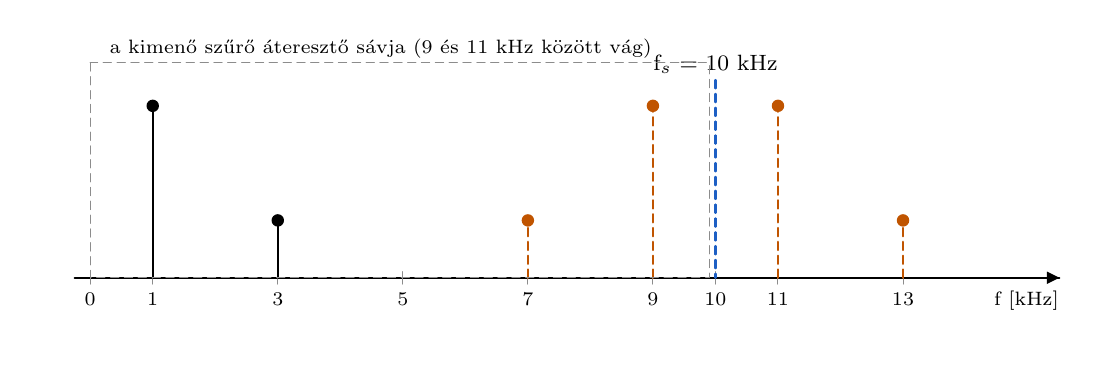
\begin{tikzpicture}[x=0.01985cm,y=-0.01985cm,line cap=round,line join=round]
\useasboundingbox (0,0) rectangle (680,200);
\path[draw=black,line width=0.7pt] (30,160) -- (660,160);
\path[fill=black,draw=none] (660,160) -- (652,156) -- (652,164) -- cycle;
\path[draw=black!45,line width=0.35pt] (40,156) -- (40,164);
\node[anchor=base,inner sep=0pt,font=\scriptsize] at (40,178) {0};
\path[draw=black!45,line width=0.35pt] (80,156) -- (80,164);
\node[anchor=base,inner sep=0pt,font=\scriptsize] at (80,178) {1};
\path[draw=black!45,line width=0.35pt] (160,156) -- (160,164);
\node[anchor=base,inner sep=0pt,font=\scriptsize] at (160,178) {3};
\path[draw=black!45,line width=0.35pt] (240,156) -- (240,164);
\node[anchor=base,inner sep=0pt,font=\scriptsize] at (240,178) {5};
\path[draw=black!45,line width=0.35pt] (320,156) -- (320,164);
\node[anchor=base,inner sep=0pt,font=\scriptsize] at (320,178) {7};
\path[draw=black!45,line width=0.35pt] (400,156) -- (400,164);
\node[anchor=base,inner sep=0pt,font=\scriptsize] at (400,178) {9};
\path[draw=black!45,line width=0.35pt] (440,156) -- (440,164);
\node[anchor=base,inner sep=0pt,font=\scriptsize] at (440,178) {10};
\path[draw=black!45,line width=0.35pt] (480,156) -- (480,164);
\node[anchor=base,inner sep=0pt,font=\scriptsize] at (480,178) {11};
\path[draw=black!45,line width=0.35pt] (560,156) -- (560,164);
\node[anchor=base,inner sep=0pt,font=\scriptsize] at (560,178) {13};
\node[anchor=base east,inner sep=0pt,font=\scriptsize] at (660,178) {f [kHz]};
\path[draw=black,line width=0.8pt] (80,160) -- (80,50);
\path[fill=black,draw=none] (80,50) circle[radius=0.079cm];
\path[draw=black,line width=0.8pt] (160,160) -- (160,123.3);
\path[fill=black,draw=none] (160,123.3) circle[radius=0.079cm];
\path[draw=cB,line width=0.8pt,dash pattern=on 3pt off 2pt] (320,160) -- (320,123.3);
\path[fill=cB,draw=none] (320,123.3) circle[radius=0.079cm];
\path[draw=cB,line width=0.8pt,dash pattern=on 3pt off 2pt] (400,160) -- (400,50);
\path[fill=cB,draw=none] (400,50) circle[radius=0.079cm];
\path[draw=cB,line width=0.8pt,dash pattern=on 3pt off 2pt] (480,160) -- (480,50);
\path[fill=cB,draw=none] (480,50) circle[radius=0.079cm];
\path[draw=cB,line width=0.8pt,dash pattern=on 3pt off 2pt] (560,160) -- (560,123.3);
\path[fill=cB,draw=none] (560,123.3) circle[radius=0.079cm];
\path[draw=cA,line width=0.8pt,dash pattern=on 3pt off 2pt] (440,33.5) -- (440,160);
\node[anchor=base,inner sep=0pt,font=\footnotesize] at (440,27.5) {f$_s$ = 10 kHz};
\path[draw=black!45,line width=0.35pt,dash pattern=on 3pt off 2pt] (40,22.5) rectangle (436,160);
\node[anchor=base west,inner sep=0pt,font=\scriptsize] at (52,16.5) {a kimenő szűrő áteresztő sávja (9 és 11 kHz között vág)};
\end{tikzpicture}\end{center}


{\footnotesize\sffamily Forrás: Koma gyak6/4 (ZH-felkészítő) $\cdot$ 5-ösöm 3. fejezet $\cdot$ azonosítók: kg06\_4. Címkék: vizsga, beugró}
\end{feladat}
\begin{keresunk}
\begin{itemize}
\item a) $f_{AA}$ (a bemenő (antialiasing) szűrő határfrekvenciája) és $f_R$ (a visszaállító szűrő határfrekvenciája)
\item b) $f_s$ (mintavételi frekvencia)
\end{itemize}
\end{keresunk}
\begin{jeloles}
\begin{jeltabla}
$f_{AA}$ & a bemenő (antialiasing) szűrő határfrekvenciája & \emph{keresett}\\
$f_R$ & a visszaállító szűrő határfrekvenciája & \emph{keresett}\\
$f_s$ & mintavételi frekvencia & \emph{keresett}\\
\end{jeltabla}
\par\smallskip\textbf{Adott még:}
\begin{itemize}
\item négyszögjel: komponensek $1,3,5,7,9,\ldots$ kHz (páratlan felharmonikusok)
\item kimenet: $\{1;3;7;9\}$ kHz
\end{itemize}
\end{jeloles}
\begin{elmelet}[Miért így? Egyszerűen]
\textbf{Miért csak páratlan felharmonikusok vannak?}\par A szimmetrikus négyszögjel félhullám-szimmetrikus, ezért a Fourier-sorában csak páratlan harmonikusok vannak.

\textbf{Honnan tudjuk, hogy a 7 és a 9 álkép?}\par Az $5$ kHz hiányzik, tehát a bemenő szűrő $5$ kHz alatt vág. Akkor a $7$ és a $9$ sem juthatott át, csak a mintavétel hozhatta létre.
\end{elmelet}
\begin{elmelet}[Felhasznált elmélet]
\textbf{Álképek.} Egy $f$ frekvenciájú komponens a mintavétel után az $n f_s\pm f$ frekvenciákon is megjelenik.
\end{elmelet}

\lepes{A bemenő szűrő}
A $3$ kHz átjut, az $5$ kHz nem.

\begin{center}\adjustbox{max width=\linewidth}{$\displaystyle 3\ \text{kHz}<f_{AA}<5\ \text{kHz}$}\end{center}
\jegyzet{ellenőrzés}{a 3 kHz átjut, az 5 kHz nem}

\lepes{A mintavételi frekvencia}
A mintavétel után csak $1$ és $3$ kHz álképei lehetnek. A $7$ és a $9$ kHz ezek közül kettő: $f_s-3=7$ és $f_s-1=9$.

\begin{center}\adjustbox{max width=\linewidth}{$\displaystyle f_s-3=7\quad\text{és}\quad f_s-1=9\ \Longrightarrow\ f_s=10\ \text{kHz}$}\end{center}
\jegyzet{definíció}{a 7 és a 9 kHz csak álkép lehet}

\begin{center}\adjustbox{max width=\linewidth}{$\displaystyle f_s=8:\ 8-3=5\ \text{kHz is megjelenne}$}\end{center}
\jegyzet{ellenőrzés}{rossz}

\begin{center}\adjustbox{max width=\linewidth}{$\displaystyle f_s=12:\ 12-3=9,\ 12-1=11\ \text{kHz, a 7 hiányozna}$}\end{center}
\jegyzet{ellenőrzés}{rossz}

\lepes{A visszaállító szűrő}
$f_s=10$ kHz-nél a következő álképek $11$ és $13$ kHz. A $9$ átjut, a $11$ nem.

\begin{center}\adjustbox{max width=\linewidth}{$\displaystyle 9\ \text{kHz}<f_R<11\ \text{kHz}$}\end{center}
\jegyzet{ellenőrzés}{a 9 átjut, a $10+1=11$ nem}
\begin{eredmeny}

\begin{center}\adjustbox{max width=\linewidth}{$\displaystyle 3<f_{AA}<5\ \text{kHz}\qquad 9<f_R<11\ \text{kHz}\qquad f_s=10\ \text{kHz}$}\end{center}
\end{eredmeny}
\begin{tipp}[Ellenőrzés]
\begin{itemize}
\item A kimenet $f_s=10$ kHz-nél: $1$, $3$ (eredeti), $10-3=7$, $10-1=9$ (álkép), a $11$ és $13$ levágva. Pontosan a megadott lista.
\end{itemize}
\end{tipp}
\begin{figyelem}[Tipikus hibák]
\begin{itemize}
\item Azt hiszik, a $7$ és a $9$ kHz a négyszögjel saját felharmonikusa. Az $5$ hiánya miatt ez lehetetlen.
\end{itemize}
\end{figyelem}
\begin{tipp}[Kapcsolat és analógia]

\par\noindent{\small\renewcommand{\arraystretch}{1.25}\begin{tabularx}{\linewidth}{@{}>{\raggedright\arraybackslash}X>{\raggedright\arraybackslash}X@{}}\toprule
2.12 (túlvezérlés) & ugyanez a gondolatmenet: a hiányzó és a megjelenő komponensekből kell visszakövetkeztetni\\
\bottomrule\end{tabularx}}\par
\end{tipp}


% ------------------------------------------------------------------
\section{\texorpdfstring{2.8. feladat: A kvantálási zaj spektrális viselkedése}{2.8. feladat: A kvantálási zaj spektrális viselkedése}}\label{p2_08}
\setcounter{lepes}{0}
\begin{feladat}{2.8. feladat}
Egy gyengén stacionárius jel spektrális sűrűsége $s(f)=6s_0\,(1-|f|/(12B))$, ha $7B<|f|<10B$, különben zérus. a) Mekkora a legkisebb $f_s$, ha a D/A utáni szűrő aluláteresztő? b) Ha a szűrő tetszőleges? c) Azonos átalakítókkal melyik esetben jobb a jel-zaj viszony? d) Mi változik, ha az a) sűrűségű mintákból a b) szűrővel állítjuk vissza a jelet?

{\footnotesize\sffamily Forrás: OneDrive 2.4 $\cdot$ Koma gyak2/4 $\cdot$ Marosi ik.5 (más számokkal) $\cdot$ azonosítók: pd02\_4, kg02\_4, mg2\_3. Címkék: nehezebb}
\end{feladat}
\begin{keresunk}
\begin{itemize}
\item a), b) $f_s$ (mintavételi frekvencia)
\item c), d) a zajteljesítmények aránya
\end{itemize}
\end{keresunk}
\begin{jeloles}
\begin{jeltabla}
$B$ & a jel sávszélessége & \\
$f_s$ & mintavételi frekvencia & \emph{keresett}\\
$s$ & a jel spektrális sűrűsége, s(f) & \\
$f$ & frekvencia (a spektrum változója) & \\
$s_0$ & a jel spektrális sűrűsége, s(f) & \\
$f_H$ & a jel legnagyobb frekvenciája & \\
$k$ & a Nyquist-zóna sorszáma a sáváteresztő mintavételnél & \\
$f_L$ & a jel legkisebb frekvenciája & \\
$P$ & a visszaállító szűrőn átjutó kvantálási zaj teljesítménye & \\
$M$ & a kvantálási zaj teljesítménye a teljes $f_s$ szélességben & \\
$f_{s,a}$ & a legkisebb $f_s$ aluláteresztő visszaállító szűrővel & \\
$f_{s,b}$ & a legkisebb $f_s$ tetszőleges visszaállító szűrővel & \\
$P_\varepsilon$ & a jel sávjába eső kvantálási zaj teljesítménye & \\
\end{jeltabla}
\par\smallskip\textbf{Adott még:}
\begin{itemize}
\item sáv: $7B\ldots10B$, szélessége $3B$
\end{itemize}
\end{jeloles}
\begin{elmelet}[Miért így? Egyszerűen]
\textbf{Miért $20B/3$ a b) eset?}\par $\lfloor10B/3B\rfloor=3$, és $k=3$-ra $2\cdot10B/3\le f_s\le2\cdot7B/2$, azaz $6{,}67B\le f_s\le7B$. A legkisebb $20B/3$.

\textbf{Miért függ a zaj a szűrőtől?}\par A kvantálási zaj fehér, $1/f_s$ sűrűségű. Amennyi sávot a szűrő átenged, annyi zajt kapunk (A5).
\end{elmelet}
\begin{elmelet}[Felhasznált elmélet]
\textbf{Kvantálási zaj.} A kvantálási zaj fehér, a $0\ldots f_s$ sávban egyenletesen oszlik el: a visszaállító szűrőn átjutó része a szűrő sávszélességével arányos.
\begin{center}\adjustbox{max width=\linewidth}{$\displaystyle P_\varepsilon=\frac{1}{f_s}M(\varepsilon^2)\int|H(f)|^2\mathrm df$}\end{center}

\end{elmelet}

\lepes{Mintavételi frekvenciák}
Aluláteresztővel $2f_H$, tetszőleges szűrővel a sáváteresztő képlet $k=3$-ra.

\begin{center}\adjustbox{max width=\linewidth}{$\displaystyle \text{a) } f_s=2\cdot10B=20B$}\end{center}
\jegyzet{tétel}{$f_H=10B$}

\begin{center}\adjustbox{max width=\linewidth}{$\displaystyle \text{b) } \frac{20B}{3}\le f_s\le\frac{14B}{2}=7B\ \Longrightarrow\ f_s=\frac{20B}{3}$}\end{center}
\jegyzet{behelyettesítés}{$k=3$: $2f_H/3$ és $2f_L/2$}

\lepes{Zajteljesítmények}
A szűrő átengedett sávja a) $2\cdot10B=20B$, b) $2\cdot3B=6B$ (két oldal).

\begin{center}\adjustbox{max width=\linewidth}{$\displaystyle \text{a) } P=\frac{1}{20B}M\cdot20B=M$}\end{center}
\jegyzet{behelyettesítés}{a zaj a teljes $f_s$ szélességben egyenletes}

\begin{center}\adjustbox{max width=\linewidth}{$\displaystyle \text{b) } P=\frac{3}{20B}M\cdot6B=0{,}9\,M$}\end{center}
\jegyzet{behelyettesítés}{a b) kicsit jobb}

\begin{center}\adjustbox{max width=\linewidth}{$\displaystyle \text{d) } P=\frac{1}{20B}M\cdot6B=0{,}3\,M$}\end{center}
\jegyzet{behelyettesítés}{a sűrű minták és a keskeny szűrő együtt}

\lepes{Decibelben}
A javulás a zajteljesítmények arányából.

\begin{center}\adjustbox{max width=\linewidth}{$\displaystyle 10\lg\frac{1}{0{,}9}=0{,}46\ \text{dB}\qquad10\lg\frac{1}{0{,}3}=5{,}2\ \text{dB}$}\end{center}
\jegyzet{számérték}{a megmaradó zaj aránya az eredetihez}
\begin{eredmeny}

\begin{center}\adjustbox{max width=\linewidth}{$\displaystyle f_{s,a}=20B\qquad f_{s,b}=\tfrac{20}{3}B\qquad P_\varepsilon:\ M,\ 0{,}9M,\ 0{,}3M$}\end{center}
\end{eredmeny}
\begin{tipp}[Ellenőrzés]
\begin{itemize}
\item A Koma-jegyzet 20/20, 18/20 és 6/20 arányai ugyanezek.
\item Marosi változata (8\ldots{}10 kHz-es sáv) ugyanezt a logikát követi: azonos SNR, túlmintavételezéssel ötszörös.
\end{itemize}
\end{tipp}
\begin{figyelem}[Tipikus hibák]
\begin{itemize}
\item Egyoldalas sávszélességgel integrálnak, és fele akkora zajt kapnak.
\end{itemize}
\end{figyelem}


% ------------------------------------------------------------------
\section{\texorpdfstring{2.9. feladat: 19\ldots{}25 kHz-es jel és a túlmintavételezés hatása}{2.9. feladat: 19…25 kHz-es jel és a túlmintavételezés hatása}}\label{p2_09}
\setcounter{lepes}{0}
\begin{feladat}{2.9. feladat}
Egy valós jel a $19$ és $25$ kHz közötti sávon kívül nem tartalmaz komponenst. a) Mi a legkisebb $f_s$, amelynél elvileg tökéletesen visszaállítható? b) Hány dB-lel javul a jel-zaj viszony, ha a határfrekvencia kétszeresével ($50$ kHz) veszünk mintát, ugyanazzal a kvantálóval és szűrővel?

{\footnotesize\sffamily Forrás: TMIT gyak01 P.1.3 $\cdot$ azonosító: tg01\_P13. Címkék: nehezebb}
\end{feladat}
\begin{keresunk}
\begin{itemize}
\item a) $f_{s,\min}$ (a legkisebb mintavételi frekvencia)
\item b) $\Delta\text{SNR}$ (a jel-zaj viszony változása)
\end{itemize}
\end{keresunk}
\begin{jeloles}
\begin{jeltabla}
$\ca{f_L}$ & a jel legkisebb frekvenciája & $19$\\
$\cb{f_H}$ & a jel legnagyobb frekvenciája & $25$\,kHz\\
$\cc{B}$ & a jel sávszélessége & $6$\,kHz\\
$f_{s,\min}$ & a legkisebb mintavételi frekvencia & \emph{keresett}\\
$f_s$ & mintavételi frekvencia & \\
$k$ & a Nyquist-zóna sorszáma: a frekvenciatengelyt $f_s/2$ széles sávokra osztjuk, és $k$ annak a sávnak a sorszáma, amelybe a jel teljes sávja beleesik & \\
$k_{\max}$ & a legnagyobb szóba jöhető zónasorszám, $\lfloor f_H/B\rfloor$ & \\
\end{jeltabla}
\end{jeloles}
\begin{elmelet}[Miért így? Egyszerűen]
\textbf{Miért nem $2B=12$ kHz a válasz?}\par $25/6$ nem egész. $12$ kHz-nél a $4\cdot12$-vel eltolt sáv ($23\ldots29$ kHz) ráesne a jelre.
\end{elmelet}
\begin{elmelet}[Felhasznált elmélet]
\textbf{Sáváteresztő mintavétel.} Ha a jel csak $f_L$ és $f_H$ között van ($B=f_H-f_L$), a megengedett mintavételi frekvenciák egész $k$-ra, $1\le k\le\lfloor f_H/B\rfloor$:
\begin{center}\adjustbox{max width=\linewidth}{$\displaystyle \frac{2f_H}{k}\le f_s\le\frac{2f_L}{k-1}$}\end{center}


\textbf{Túlmintavételezés.} A jel-zaj viszonyban a $10\lg(f_s/2B)$ tag: ha ugyanazzal a kvantálóval és szűrővel sűrűbben mintázunk, a kvantálási zaj szélesebb sávra terül szét, és kevesebb jut a szűrő sávjába.
\end{elmelet}

\lepes{Mit jelent a $k$? A Nyquist-zóna sorszáma}
A mintavétel után a spektrum $f_s$-enként ismétlődik. Osszuk fel a frekvenciatengelyt $f_s/2$ széles sávokra (Nyquist-zónákra): $0\ldots f_s/2$ az első, $f_s/2\ldots f_s$ a második, és így tovább. \textbf{$k$ annak a zónának a sorszáma, amelybe a jel teljes sávja beleesik:} $(k-1)\,f_s/2\le {\ca{f_L}}$ és ${\cb{f_H}}\le k\,f_s/2$. A két egyenlőtlenséget $f_s$-re rendezve kapjuk a megengedett tartományt, $2{\cb{f_H}}/k\le f_s\le2{\ca{f_L}}/(k-1)$. A $k=1$ eset a szokásos aluláteresztő mintavétel ($f_s\ge2{\cb{f_H}}$). Mivel a zóna nem lehet keskenyebb a jelnél ($f_s/2\ge {\cc{B}}$), $k$ legfeljebb ${\cb{f_H}}/{\cc{B}}$ lehet, lefelé kerekítve: $k_{\max}=\lfloor {\cb{f_H}}/{\cc{B}}\rfloor$.

\lepes{A legkisebb mintavételi frekvencia}
$k=4$-re behelyettesítünk.
\behely{\bh{\ca{f_L}}{\ca{19}} \bh{\cb{f_H}}{\cb{25\un{kHz}}}}

\begin{center}\adjustbox{max width=\linewidth}{$\displaystyle \frac{2\cdot{\cb{25}}}{4}\le f_s\le\frac{2\cdot{\ca{19}}}{3}\ \Longrightarrow\ 12{,}5\le f_s\le12{,}67\ \text{kHz}$}\end{center}
\jegyzet{behelyettesítés}{$k=\lfloor25/6\rfloor=4$}

\lepes{A jel-zaj viszony változása}
Csak az $f_s/2{\cc{B}}$ tag változik, mert a kvantáló, a csúcstényező és a szűrő ugyanaz.

\begin{center}\adjustbox{max width=\linewidth}{$\displaystyle \Delta\text{SNR}=10\lg\frac{50}{f_{s,\min}}$}\end{center}
\jegyzet{átalakítás}{a két $10\lg(f_s/2B)$ tag különbsége}

\begin{center}\adjustbox{max width=\linewidth}{$\displaystyle 10\lg\frac{50}{12{,}67}=5{,}96\ \text{dB}\ \ldots\ 10\lg\frac{50}{12{,}5}=6{,}02\ \text{dB}$}\end{center}
\jegyzet{számérték}{a tartomány két végére}
\begin{eredmeny}

\begin{center}\adjustbox{max width=\linewidth}{$\displaystyle f_{s,\min}=12{,}5\ \text{kHz}\qquad\Delta\text{SNR}\approx6\ \text{dB}$}\end{center}
\end{eredmeny}
\begin{tipp}[Ellenőrzés]
\begin{itemize}
\item $f_s=12{,}5$: $-25+4\cdot12{,}5=25$, épp érintkezik. $-19+3\cdot12{,}5=18{,}5<19$, nem lapolódik.
\item $6$ dB ugyanannyi, mint egy bit, mert négyszeres a túlmintavételezés.
\end{itemize}
\end{tipp}
\begin{figyelem}[Tipikus hibák]
\begin{itemize}
\item $2B=12$ kHz-et adnak meg. A sáváteresztő táblázat nélkül ez nem derül ki.
\end{itemize}
\end{figyelem}


% ------------------------------------------------------------------
\section{\texorpdfstring{2.10. feladat: Túlmintavételezés interpolált mintákkal}{2.10. feladat: Túlmintavételezés interpolált mintákkal}}\label{p2_10}
\setcounter{lepes}{0}
\begin{feladat}{2.10. feladat}
A $15$ kHz sávszélességű jelet $44$ kHz-cel mintavételezzük, $20$ bites mintákkal. A visszaállító D/A átalakító $16$ bites, a szűrő ideális aluláteresztő. a) Mennyit javul a jel-zaj viszony, ha négyszeres sűrűségű interpolált mintákkal állítjuk vissza? b) Mire számíthatunk, ha a szűrő $15$ kHz-es töréspontú elsőfokú aluláteresztő?

{\footnotesize\sffamily Forrás: TMIT gyak01 P.1.4 $\cdot$ azonosító: tg01\_P14}
\end{feladat}
\begin{keresunk}
\begin{itemize}
\item a) $\text{SNR}$ (jel-zaj viszony) előtte és utána
\item b) a szivárgó komponensek
\end{itemize}
\end{keresunk}
\begin{jeloles}
\begin{jeltabla}
$\ca{B}$ & a jel sávszélessége & $15$\,kHz\\
$\cb{f_s}$ & mintavételi frekvencia & $44$\,kHz\\
$\cc{n}$ & a kvantáló bitszáma & $16$\,bit\\
$C$ & csúcstényező & \\
$S$ & a jel teljesítménye & \\
$N$ & a kvantálási zaj teljesítménye & \\
$H$ & a szűrő átvitele & \\
\end{jeltabla}
\end{jeloles}
\begin{elmelet}[Miért így? Egyszerűen]
\textbf{Miért a D/A bitszáma számít?}\par A pontos ($20$ bites) mintákat a $16$ bites D/A kerekíti. A visszaállított jel kvantálási zaját ez a kerekítés adja.

\textbf{Miért segít az interpoláció?}\par A közbenső minták számolhatók a pontos mintákból. A D/A négyszer sűrűbben dolgozik, így a zaj négyszer szélesebb sávra oszlik szét.
\end{elmelet}
\begin{elmelet}[Felhasznált elmélet]
\textbf{Jel-zaj viszony.} Egyenletes kvantálásnál, $C$ csúcstényezőjű, teljes kivezérlésű jelre, $n$ bittel, $B$ sávú visszaállító szűrővel:
\begin{center}\adjustbox{max width=\linewidth}{$\displaystyle \text{SNR}_{\mathrm{dB}}=10\lg\frac{3}{C^2}+10\lg\frac{f_s}{2B}+6{,}02\,n$}\end{center}

\end{elmelet}

\lepes{Kiindulási jel-zaj viszony}
Szinuszra vonatkoztatva ($C^2=2$).
\behely{\bh{\ca{B}}{\ca{15\un{kHz}}}}

\begin{center}\adjustbox{max width=\linewidth}{$\displaystyle \frac SN=\frac32\cdot\frac{44}{2\cdot{\ca{15}}}\cdot2^{32}$}\end{center}
\jegyzet{behelyettesítés}{$C^2=2$, $f_s=44$, $B=15$ kHz, $n=16$}

\begin{center}\adjustbox{max width=\linewidth}{$\displaystyle 10\lg\frac SN\approx99{,}8\ \text{dB}$}\end{center}
\jegyzet{számérték}{$1{,}76+1{,}66+96{,}3$}

\lepes{Négyszeres sűrűséggel}
Csak az ${\cb{f_s}}/2{\ca{B}}$ tag változik.
\behely{\bh{\ca{B}}{\ca{15\un{kHz}}} \bh{\cb{f_s}}{\cb{44\un{kHz}}}}

\begin{center}\adjustbox{max width=\linewidth}{$\displaystyle \frac SN=\frac32\cdot\frac{4\cdot{\cb{44}}}{2\cdot{\ca{15}}}\cdot2^{32}\ \Longrightarrow\ 105{,}8\ \text{dB}$}\end{center}
\jegyzet{behelyettesítés}{+6 dB, mint egy bit}

\lepes{Elsőfokú szűrővel}
A legalacsonyabb szivárgó komponens ${\cb{f_s}}-{\ca{15}}$ kHz-nél van.

\begin{center}\adjustbox{max width=\linewidth}{$\displaystyle {\cb{44}}-{\ca{15}}=29\ \text{kHz}\qquad 4\cdot{\cb{44}}-{\ca{15}}=161\ \text{kHz}$}\end{center}
\jegyzet{számérték}{interpolációval sokkal messzebb}

\begin{center}\adjustbox{max width=\linewidth}{$\displaystyle |H(161)|\approx\frac{15}{161}\approx0{,}093\ \Longrightarrow\ \approx20\ \text{dB}$}\end{center}
\jegyzet{közelítés}{elsőfokú szűrő, 20 dB/dekád}
\begin{eredmeny}

\begin{center}\adjustbox{max width=\linewidth}{$\displaystyle 99{,}8\ \text{dB}\ \longrightarrow\ 105{,}8\ \text{dB}\qquad\text{szivárgás } 29\ \text{kHz helyett } 161\ \text{kHz-től, ott kb. 20 dB csillapítás}$}\end{center}
\end{eredmeny}
\begin{tipp}[Ellenőrzés]
\begin{itemize}
\item $10\lg4=6{,}02$ dB, és egy bit $6{,}02$ dB: a TMIT-füzet ugyanezt állapítja meg.
\end{itemize}
\end{tipp}
\begin{figyelem}[Tipikus hibák]
\begin{itemize}
\item A $20$ bites forrással számolnak. A kimenet pontosságát a $16$ bites D/A korlátozza.
\end{itemize}
\end{figyelem}


% ------------------------------------------------------------------
\section{\texorpdfstring{2.11. feladat: Az előadás felvétele: 4 kHz, 9 kHz, 14 bit}{2.11. feladat: Az előadás felvétele: 4 kHz, 9 kHz, 14 bit}}\label{p2_11}
\setcounter{lepes}{0}
\begin{feladat}{2.11. feladat}
Az előadást digitális hangtechnikával rögzítjük. A mikrofon jelét $4$ kHz-es ideális aluláteresztő szűri, a mintavétel $9$ kHz, a kvantálás $14$ bites, egyenletes. a) Sikerül-e így tökéletes felvétel? b) Ha nem, miért? c) Kell-e szűrő a bemeneten és a kimeneten? d) Milyen hallható változást okoz, ha minden mintából elhagyjuk a legkisebb helyiértékű $6$ bitet? e) Ha a tréfás hallgató $26$ dB-lel hangosabban beszél, hányszoros a teljesítményigénye?

{\footnotesize\sffamily Forrás: Marosi „Példák \#1” 2. (2016) $\cdot$ azonosító: mgP\_2. Címkék: vizsga}
\end{feladat}
\begin{keresunk}
\begin{itemize}
\item a)\ldots{}c) szövegesen
\item d) $\Delta\text{SNR}$ (a jel-zaj viszony változása)
\item e) teljesítményarány
\end{itemize}
\end{keresunk}
\begin{jeloles}
\begin{jeltabla}
$\ca{B}$ & a jel sávszélessége & $4$\,kHz\\
$\cb{f_s}$ & mintavételi frekvencia & $9$\,kHz\\
$\cc{n}$ & a kvantáló bitszáma & $14$\,bit\\
$i$ & tetszőleges pozitív egész & \\
$f$ & a bemenő jel frekvenciája & \\
\end{jeltabla}
\end{jeloles}
\begin{elmelet}[Miért így? Egyszerűen]
\textbf{Miért nem tökéletes, ha $f_s>2B$?}\par Mintavétel szempontjából rendben van, de a $4$ kHz-es sávkorlát a beszéd magasabb összetevőit levágja, és a kvantálási zaj sem tűnik el soha.

\textbf{Miért $6$ dB egy bit?}\par Minden bit kétszer annyi szintet ad, a lépcső felére csökken, a zajteljesítmény negyedére. $10\lg4=6{,}02$ dB.
\end{elmelet}
\begin{elmelet}[Felhasznált elmélet]
\textbf{Jel-zaj viszony.} Egyenletes kvantálásnál, $C$ csúcstényezőjű, teljes kivezérlésű jelre, $n$ bittel, $B$ sávú visszaállító szűrővel:
\begin{center}\adjustbox{max width=\linewidth}{$\displaystyle \text{SNR}_{\mathrm{dB}}=10\lg\frac{3}{C^2}+10\lg\frac{f_s}{2B}+6{,}02\,n$}\end{center}


\textbf{Decibel.} Teljesítményarányra $10\lg$, feszültségre $20\lg$: 3 dB kétszeres, 10 dB tízszeres, 20 dB százszoros teljesítmény.
\end{elmelet}

\lepes{Tökéletes-e?}
Nem: a sávkorlát ($4$ kHz az érthetőséghez elég) és a kvantálási zaj miatt. Átlapolódás nincs, mert $9>2\cdot4$.

\lepes{Szűrők}
A bemeneten kell, különben a $4{,}5$ kHz feletti zaj és hang átlapolódna. A kimeneten is kell, mert a D/A után ott vannak az $i\cdot9\pm f$ kHz-es másolatok ($i$ tetszőleges pozitív egész, $f$ a hang egy összetevőjének frekvenciája).

\lepes{6 bit elhagyása}
Minden bit $6$ dB.

\begin{center}\adjustbox{max width=\linewidth}{$\displaystyle \Delta\text{SNR}=6\cdot6{,}02=36\ \text{dB}\qquad 2^{12}=4096\approx4000\text{-szeres zajteljesítmény}$}\end{center}
\jegyzet{számérték}{sistergés}

\lepes{26 dB hangosabban}
Teljesítményarány a decibelből.

\begin{center}\adjustbox{max width=\linewidth}{$\displaystyle 10^{26/10}=10^{2{,}6}\approx398\approx400$}\end{center}
\jegyzet{átalakítás}{dB-ből teljesítményarány}
\begin{eredmeny}

\begin{center}\adjustbox{max width=\linewidth}{$\displaystyle \text{d) } -36\ \text{dB}\ (\approx4000\times\ \text{zaj})\qquad\text{e) } \approx400\times$}\end{center}
\end{eredmeny}
\begin{tipp}[Ellenőrzés]
\begin{itemize}
\item $26$ dB $=20+6$ dB, azaz $100\cdot4=400$: a fejszámolás egyezik.
\end{itemize}
\end{tipp}
\begin{figyelem}[Tipikus hibák]
\begin{itemize}
\item $20\lg$-gel számolnak a teljesítménynél, és $20$-szorost kapnak.
\end{itemize}
\end{figyelem}


% ------------------------------------------------------------------
\section{\texorpdfstring{2.12. feladat: Túlvezérlés: honnan jön a 3,5 kHz?}{2.12. feladat: Túlvezérlés: honnan jön a 3,5 kHz?}}\label{p2_12}
\setcounter{lepes}{0}
\begin{feladat}{2.12. feladat}
Egy $8$ kHz-es mintavételi frekvenciájú rendszer egy $1{,}5$ kHz-es szinuszt hibátlanul visz át. Ha a bemenő amplitúdó $2$ V fölé nő, a kimeneten egy kis $3{,}5$ kHz-es komponens is megjelenik (a visszaállító szűrő $4$ kHz-es, jó minőségű aluláteresztő). a) Magyarázható-e ez a rendszer bemenő fokozatának túlvezérlésével? b) Milyen további frekvenciák lehetnek a kimeneten?

{\footnotesize\sffamily Forrás: Marosi „Példák \#1” 2/b (2016) $\cdot$ azonosító: mgP\_2b. Címkék: vizsga, nehezebb}
\end{feladat}
\begin{keresunk}
\begin{itemize}
\item a) magyarázat
\item b) a $4$ kHz alatti komponensek
\end{itemize}
\end{keresunk}
\begin{jeloles}
\begin{jeltabla}
$\ca{f_s}$ & mintavételi frekvencia & $8$\,kHz\\
$\cb{f}$ & a bemenő jel frekvenciája & $1{,}5$\,kHz\\
$\cc{f_R}$ & a visszaállító szűrő határfrekvenciája & $4$\,kHz\\
$f_k$ & a négyszögjel egy felharmonikusának frekvenciája & \\
$k$ & nemnegatív egész, a 2k+1 a felharmonikus (páratlan) sorszáma & \\
$n$ & tetszőleges egész szám (hányadik mintavételi többszörös) & \\
\end{jeltabla}
\end{jeloles}
\begin{elmelet}[Miért így? Egyszerűen]
\textbf{Miért páratlan felharmonikusok?}\par A szimmetrikus vágás (túlvezérlés) a szinuszt a négyszög felé torzítja, amelynek csak páratlan felharmonikusai vannak.

\textbf{Hogyan lesz $4{,}5$ kHz-ből $3{,}5$ kHz?}\par A $3\cdot1{,}5=4{,}5$ kHz az $f_s/2$ felett van, álképe $8-4{,}5=3{,}5$ kHz (A2).
\end{elmelet}
\begin{elmelet}[Felhasznált elmélet]
\textbf{Álképek.} Egy $f$ frekvenciájú komponens a mintavétel után az $n f_s\pm f$ frekvenciákon is megjelenik.
\end{elmelet}

\lepes{A torzítás komponensei}
Erős túlvezérlésnél a jel a négyszöghöz közelít.

\begin{center}\adjustbox{max width=\linewidth}{$\displaystyle f_k=(2k+1)\cdot{\cb{1{,}5}}\ \text{kHz}={\cb{1{,}5}};\ 4{,}5;\ 7{,}5;\ 10{,}5;\ \ldots$}\end{center}
\jegyzet{definíció}{a négyszögjel páratlan felharmonikusai}

\lepes{Mintavétel után}
Minden komponensnek $n\cdot8\pm f_k$ álképe lesz.

\begin{center}\adjustbox{max width=\linewidth}{$\displaystyle 8-4{,}5=3{,}5\qquad8-7{,}5=0{,}5\qquad10{,}5-8=2{,}5\ \text{kHz}$}\end{center}
\jegyzet{számérték}{$n\cdot8\pm f_k$, a 4 kHz alattiak}

\begin{center}\adjustbox{max width=\linewidth}{$\displaystyle 16-13{,}5=2{,}5\qquad16-16{,}5=-0{,}5\to0{,}5\ \text{kHz}$}\end{center}
\jegyzet{ellenőrzés}{a magasabbak ugyanezekre esnek}
\begin{eredmeny}

\begin{center}\adjustbox{max width=\linewidth}{$\displaystyle \text{a) igen}\qquad\text{b) } 0{,}5;\ 1{,}5;\ 2{,}5;\ 3{,}5\ \text{kHz}$}\end{center}
\end{eredmeny}
\begin{tipp}[Ellenőrzés]
\begin{itemize}
\item Marosi táblai megoldása ugyanezt a négy frekvenciát adja.
\item Mind $1$ kHz-es rácson van, félúton: ez az $n\cdot8\pm(2k+1)\cdot1{,}5$ alakból következik.
\end{itemize}
\end{tipp}
\begin{figyelem}[Tipikus hibák]
\begin{itemize}
\item Csak a $4{,}5$ kHz álképét keresik, a $7{,}5$ és a $10{,}5$ kHz-es felharmonikust elfelejtik.
\end{itemize}
\end{figyelem}
\begin{tipp}[Kapcsolat és analógia]

\par\noindent{\small\renewcommand{\arraystretch}{1.25}\begin{tabularx}{\linewidth}{@{}>{\raggedright\arraybackslash}X>{\raggedright\arraybackslash}X@{}}\toprule
2.2 (egyenirányítás) & páros felharmonikusok, $n\cdot8\pm k\cdot3{,}6$ kHz\\
2.7 (négyszögjel) & ugyanez a felharmonikus-logika szándékos négyszögjellel\\
\bottomrule\end{tabularx}}\par
\end{tipp}

% Generálva: html/build_tex.js (ch06.js). Kézzel ne szerkeszd, a forrás a html/data mappa.
\setcounter{chapter}{5}
\chapter{\texorpdfstring{Kódolástechnika}{Kódolástechnika}}\label{f6}
A kódolás négy fajtájából kettővel számolunk: a forráskódolással (mennyire tömöríthető a forrás) és a hibavédő kódolással (hány hibát jelez és javít a kód). Az anyag a Kódolás előadás 12 tábláján alapul, koma E2 jegyzetével és G3, G6 gyakorlatával összevetve. A [bizonytalan] jelölésű részek megerősítésre várnak.

\section{Alapok, egyszerűen}
\subsection{\texorpdfstring{A1. A kódolás fajtái, egyszerűen}{A1. A kódolás fajtái, egyszerűen}}\label{a6-fajtak}
A táblán négy fajta szerepel (tábla 1): \textbf{tömörítő kódolás} (forráskódolás), \textbf{hibavédő kódolás} (ezen belül hibajelző és hibajavító), \textbf{titkosító kódolás}, és külön nyíllal a \textbf{vonali kódolás}.

Gondolj egy csomagküldésre. A tömörítés a vákuumozás: ugyanaz a tartalom kisebb dobozban. A hibavédő kódolás a buborékfólia: plusz anyag, ami nem tartalom, de megvédi a sérüléstől. A titkosítás a lakat: csak az nyitja ki, akinek kulcsa van. A vonali kódolás a futár menetrendje: nem a tartalomról szól, hanem arról, hogy az adó és a vevő egy ütemre dolgozzon.

Mire jó? A tömörítő és a hibavédő kódolás ellentétes irányba húz: az egyik elveszi a fölösleget, a másik szándékosan tesz hozzá (koma E2: „a tömörítés kárára további biteket adunk hozzá”). Ezért külön lépésként kezeljük őket.

A táblán a vonali kódolás előtt nyíl áll, a többi előtt felsorolásjel. Koma jegyzete szerint a vonali kódolás folytonos, a vonalon egy bit hosszát jelzi, és szinkronban tartja az adót és a vevőt, ezért más jellegű, mint a többi.

\subsection{\texorpdfstring{A2. Kód, kódszó, prefixmentesség}{A2. Kód, kódszó, prefixmentesség}}\label{a6-kod}
A forrás ABC ($\mathcal F$) elemei a \textbf{forrásszimbólumok}, a kód ABC elemei a \textbf{kódszimbólumok} (nálunk a 0 és az 1). A kódolás minden forrásszimbólumhoz egy kódszót rendel. \textbf{A kódszavak összessége a kód} (tábla 2). Az $a_i$ szimbólum kódszavának hossza $l_i$ (szóban elhangzott).

Egy kódtól három dolgot várunk (tábla 1): legyen \textbf{egyértelműen visszaállítható}, \textbf{veszteségmentes} és \textbf{tömör}.

\textbf{Prefixmentes} (koma: prefix kód) az a kód, amelyben egyik kódszó sem eleje (prefixe) egy másiknak. A tábla példája ($01, 001, 0001, \dots, 1111111$) ilyen: a $01$ nem eleje a $001$ szónak, a $011$ szónak viszont eleje lenne (szóban elhangzott). Az ilyen kód \textbf{azonnal dekódolható}: minden kódszó végén rögtön tudjuk, melyik szimbólum volt (szóban elhangzott).

\begin{center}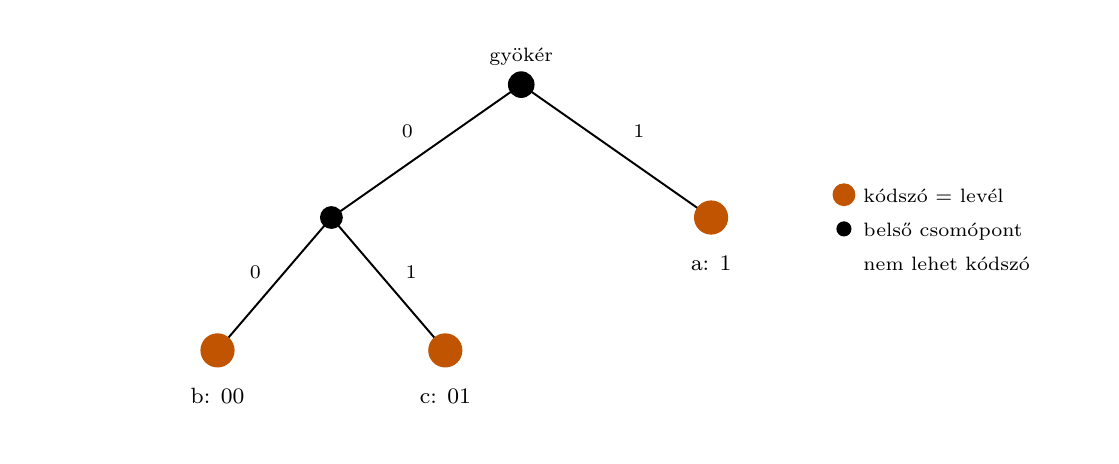
\begin{tikzpicture}[x=0.02411cm,y=-0.02411cm,line cap=round,line join=round]
\useasboundingbox (0,0) rectangle (560,215);
\path[draw=black,line width=0.7pt] (260,30) -- (160,100);
\path[draw=black,line width=0.7pt] (260,30) -- (360,100);
\path[draw=black,line width=0.7pt] (160,100) -- (100,170);
\path[draw=black,line width=0.7pt] (160,100) -- (220,170);
\node[anchor=base,inner sep=0pt,font=\scriptsize] at (200,58) {0};
\node[anchor=base,inner sep=0pt,font=\scriptsize] at (322,58) {1};
\node[anchor=base,inner sep=0pt,font=\scriptsize] at (120,132) {0};
\node[anchor=base,inner sep=0pt,font=\scriptsize] at (202,132) {1};
\path[fill=black,draw=none] (260,30) circle[radius=0.169cm];
\path[fill=black,draw=none] (160,100) circle[radius=0.145cm];
\path[fill=cB,draw=none] (360,100) circle[radius=0.217cm];
\path[fill=cB,draw=none] (100,170) circle[radius=0.217cm];
\path[fill=cB,draw=none] (220,170) circle[radius=0.217cm];
\node[anchor=base,inner sep=0pt,font=\footnotesize] at (360,128) {a: 1};
\node[anchor=base,inner sep=0pt,font=\footnotesize] at (100,198) {b: 00};
\node[anchor=base,inner sep=0pt,font=\footnotesize] at (220,198) {c: 01};
\node[anchor=base,inner sep=0pt,font=\scriptsize] at (260,18) {gyökér};
\node[anchor=base west,inner sep=0pt,font=\scriptsize] at (440,92) {kódszó = levél};
\node[anchor=base west,inner sep=0pt,font=\scriptsize] at (440,110) {belső csomópont};
\node[anchor=base west,inner sep=0pt,font=\scriptsize] at (440,128) {nem lehet kódszó};
\path[fill=cB,draw=none] (430,88) circle[radius=0.145cm];
\path[fill=black,draw=none] (430,106) circle[radius=0.096cm];
\end{tikzpicture}\end{center}

Analógia: a telefonszámok. Ha a 12 és a 123 is érvényes szám lenne, a központ már a 2 után kapcsolna, és a 123 sosem lenne hívható. A telefonszámok ezért prefixmentesek. A bináris fán ez azt jelenti, hogy minden kódszó levél, egyik sem áll egy másik útjában.

\subsection{\texorpdfstring{A3. Átlagos kódszóhossz és a fix hosszú kód}{A3. Átlagos kódszóhossz és a fix hosszú kód}}\label{a6-hossz}
Ha az $a_i$ szimbólum valószínűsége $p_i$, az átlagos kódszóhossz egy forrásszimbólumra:

\begin{center}\adjustbox{max width=\linewidth}{$\displaystyle L=\sum_{i=1}^{N} p_i\, l_i \quad [\text{bit/szimbólum}]$}\end{center}

Fix hosszú kódnál minden kódszó egyforma hosszú. $N$ szimbólumhoz annyi bit kell, hogy $2^L \ge N$ legyen, tehát $L=\lceil \log_2 N\rceil$, és ez mindig ebbe a sávba esik (tábla 3):

\begin{center}\adjustbox{max width=\linewidth}{$\displaystyle \log_2 N \le L < 1+\log_2 N$}\end{center}

Ha $N$ kettő hatványa, nincs veszteség. Ha eggyel több, majdnem egy egész bitet fizetünk ki: $N=32$ esetén 5 bit, $N=33$ esetén már 6 (6.1. példa).

A tábla javaslata: kódoljunk szimbólumpárokat. Párból $N^2$ van, egy pár kódszava $\lceil 2\log_2 N\rceil$ bit, és a kerekítés miatti fölösleg két szimbólum között oszlik meg (6.2. példa):

\begin{center}\adjustbox{max width=\linewidth}{$\displaystyle 2\log_2 N \le L^{(2)} < 1+2\log_2 N \quad\Longrightarrow\quad \log_2 N \le \frac{L^{(2)}}{2} < \frac12+\log_2 N$}\end{center}

Analógia: a csomagolás. Ha minden tárgy külön dobozba kerül, minden dobozban marad üres hely. Ha kettesével csomagolunk, az üres hely két tárgyra oszlik el, egy tárgyra legfeljebb fele annyi jut.

\subsection{\texorpdfstring{A4. Entrópia: a tömörítés alsó korlátja}{A4. Entrópia: a tömörítés alsó korlátja}}\label{a6-entropia}
Ha a szimbólumok nem egyformán gyakoriak, a gyakoribbak kaphatnak rövidebb kódszót ((2) változó szóhosszúságú kódszavak, tábla 3). A legjobb elérhető átlagos hosszt az \textbf{entrópia} adja (tábla 5):

\begin{center}\adjustbox{max width=\linewidth}{$\displaystyle H(\mathcal F)=\sum_{i=1}^{N} p_i \log_2\frac{1}{p_i}\quad[\text{bit/szimbólum}]$}\end{center}

Ha az $a_i$ kódszava kb. $\log_2(1/p_i)$ hosszú (felfelé kerekítve), akkor (tábla 5):

\begin{center}\adjustbox{max width=\linewidth}{$\displaystyle H(\mathcal F) \le L < 1+H(\mathcal F)$}\end{center}

Független szimbólumok párjára $H(\mathcal F^2)=2H(\mathcal F)$ (tábla 6, 6.5. példa), ezért a felső korlát egy szimbólumra felére csökken:

\begin{center}\adjustbox{max width=\linewidth}{$\displaystyle H(\mathcal F) \le L < \tfrac12 + H(\mathcal F)$}\end{center}

Koma jegyzete szerint $k$ szimbólumos csoportokra $H \le L < 1/k + H$, tehát az entrópia tetszőlegesen megközelíthető, csak egyre drágábban.

Analógia: a meglepetés. Ha egy esemény szinte biztos, a hír, hogy megtörtént, alig mond újat ($\log_2(1/p_i)$ kicsi). A ritka esemény híre sokat mond. Az entrópia a hírek átlagos meglepetése bitben, ennél rövidebben átlagosan nem lehet leírni a forrást.

\subsection{\texorpdfstring{A5. Kraft és McMillan: mikor megfejthető egy kód?}{A5. Kraft és McMillan: mikor megfejthető egy kód?}}\label{a6-kraft}
Ha a kódszavak hossza $l_1, \dots, l_N$, mindkét tétel ugyanazt a feltételt írja fel (tábla 4):

\begin{center}\adjustbox{max width=\linewidth}{$\displaystyle \sum_{i=1}^{N} 2^{-l_i} \le 1$}\end{center}

\textbf{McMillan-egyenlőtlenség:} ha a kód egyértelműen megfejthető, a feltétel teljesül. Ha tehát az összeg 1 fölött van, a kód biztosan nem egyértelműen megfejthető. \textbf{Kraft-egyenlőtlenség:} ha a feltétel teljesül, létezik ilyen hosszakkal prefixmentes kód (koma E2: akkor és csak akkor).

Analógia: egy torta. Egy $l$ hosszú kódszó a lehetséges bitsorozatok $2^{-l}$ részét foglalja le (minden vele kezdődő folytatást). Egy 1 bites kódszó a torta felét, egy 2 bites a negyedét viszi. Többet nem lehet szétosztani, mint amennyi torta van.

\subsection{\texorpdfstring{A6. Hibák a csatornán, BSC}{A6. Hibák a csatornán, BSC}}\label{a6-csatorna}
Kétféle hiba van (tábla 7). \textbf{Törlődéses hiba:} a vevő nem tud dönteni, nem tudja, 0 vagy 1 jött. \textbf{Tévesztés:} a vevő dönt, de rosszul, $0 \to 1$ vagy $1 \to 0$.

\begin{center}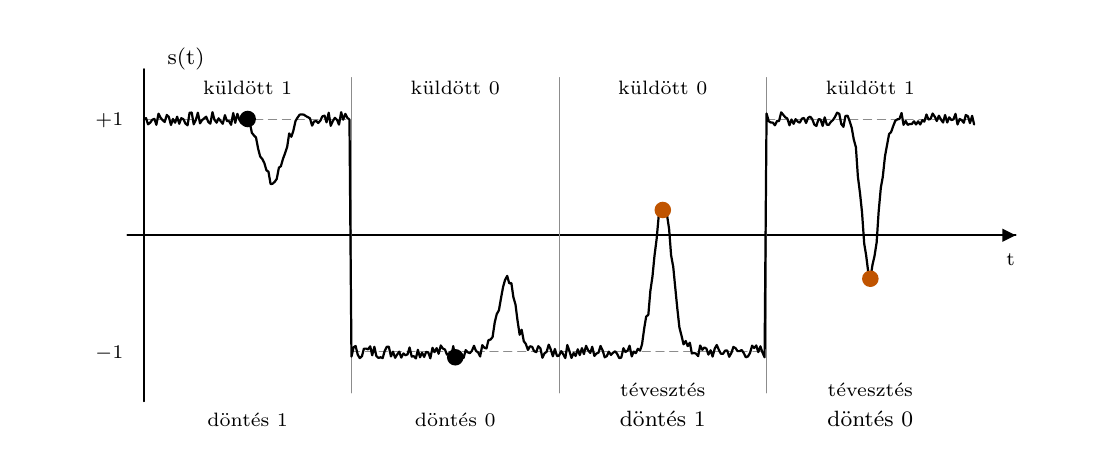
\begin{tikzpicture}[x=0.02109cm,y=-0.02109cm,line cap=round,line join=round]
\useasboundingbox (0,0) rectangle (640,250);
\path[draw=black,line width=0.7pt] (60,125) -- (595,125);
\path[fill=black,draw=none] (595,125) -- (587,121) -- (587,129) -- cycle;
\path[draw=black,line width=0.7pt] (70,25) -- (70,225);
\node[anchor=base east,inner sep=0pt,font=\scriptsize] at (58,59) {+1};
\node[anchor=base east,inner sep=0pt,font=\scriptsize] at (58,199) {$-$1};
\node[anchor=base,inner sep=0pt,font=\scriptsize] at (592,143) {t};
\node[anchor=base west,inner sep=0pt,font=\footnotesize] at (84,22) {s(t)};
\path[draw=black!45,line width=0.35pt,dash pattern=on 3pt off 2pt] (70,55) -- (195,55) (195,195) -- (320,195) (320,195) -- (445,195) (445,55) -- (570,55);
\path[draw=black!45,line width=0.35pt] (195,30) -- (195,220);
\path[draw=black!45,line width=0.35pt] (320,30) -- (320,220);
\path[draw=black!45,line width=0.35pt] (445,30) -- (445,220);
\path[draw=black,line width=0.8pt] (70,55.1) -- (71.3,54.5) -- (72.5,58.2) -- (73.8,57.2) -- (75,55.5) -- (76.3,54.9) -- (77.5,58.5) -- (78.8,51.8) -- (80,54.2) -- (81.3,55.7) -- (82.5,56.8) -- (83.8,52.6) -- (85,53.7) -- (86.3,58.6) -- (87.5,55) -- (88.8,57.2) -- (90,53.6) -- (91.3,57.9) -- (92.5,54.5) -- (93.8,55.1) -- (95,57.7) -- (96.3,58.8) -- (97.5,51.3) -- (98.8,51.1) -- (100,58.2) -- (101.3,55.5) -- (102.5,51.2) -- (103.8,57.6) -- (105,55.7) -- (106.3,54.6) -- (107.5,53.6) -- (108.8,56.8) -- (110,57.8) -- (111.3,50.9) -- (112.5,55.5) -- (113.8,57.2) -- (115,54.6) -- (116.3,56.4) -- (117.5,57.9) -- (118.8,52.7) -- (120,56.2) -- (121.3,56.3) -- (122.5,58.5) -- (123.8,51.4) -- (125,57.3) -- (126.3,51.9) -- (127.5,55.5) -- (128.8,57.6) -- (130,54.9) -- (131.3,57.1) -- (132.5,55) -- (133.8,57.1) -- (135,63.3) -- (136.3,64.9) -- (137.5,66.1) -- (138.8,72.9) -- (140,77.5) -- (141.3,79.1) -- (142.5,81.4) -- (143.8,85.9) -- (145,86.7) -- (146.3,94.2) -- (147.5,94) -- (148.8,92.8) -- (150,91.1) -- (151.3,84.3) -- (152.5,83.4) -- (153.8,78.9) -- (155,75.7) -- (156.3,71.7) -- (157.5,63.7) -- (158.8,65.7) -- (160,62.1) -- (161.3,56.2) -- (162.5,54.2) -- (163.8,52.4) -- (165,52.2) -- (166.3,52.4) -- (167.5,53.2) -- (168.8,53.9) -- (170,54.6) -- (171.3,59) -- (172.5,56.5) -- (173.8,56.2) -- (175,57.4) -- (176.3,55.9) -- (177.5,53.4) -- (178.8,53) -- (180,57) -- (181.3,51.2) -- (182.5,59.1) -- (183.8,56.2) -- (185,54.3) -- (186.3,55.5) -- (187.5,58.4) -- (188.8,50.9) -- (190,55.4) -- (191.3,51.9) -- (192.5,54.3) -- (193.8,55.3) -- (195,198.1) -- (196.3,192.5) -- (197.5,191.7) -- (198.8,197) -- (200,199) -- (201.3,197.9) -- (202.5,193.3) -- (203.8,193.3) -- (205,193.7) -- (206.3,191.9) -- (207.5,197.3) -- (208.8,192.2) -- (210,197.8) -- (211.3,198.9) -- (212.5,198.5) -- (213.8,199) -- (215,194.7) -- (216.3,192.2) -- (217.5,192.1) -- (218.8,198) -- (220,195.1) -- (221.3,198.8) -- (222.5,196.9) -- (223.8,195.1) -- (225,198.7) -- (226.3,196.2) -- (227.5,197.3) -- (228.8,196.7) -- (230,192.6) -- (231.3,198.1) -- (232.5,197.8) -- (233.8,199.2) -- (235,194) -- (236.3,198.5) -- (237.5,195.8) -- (238.8,198.3) -- (240,195.2) -- (241.3,195.7) -- (242.5,199.1) -- (243.8,192.8) -- (245,195.4) -- (246.3,193) -- (247.5,196.4) -- (248.8,191.4) -- (250,193.2) -- (251.3,193.8) -- (252.5,196.9) -- (253.8,196.2) -- (255,198.6) -- (256.3,191.8) -- (257.5,198.5) -- (258.8,198.6) -- (260,197.6) -- (261.3,196.6) -- (262.5,199) -- (263.8,194.2) -- (265,195.5) -- (266.3,196) -- (267.5,194.7) -- (268.8,191.6) -- (270,194.7) -- (271.3,195.6) -- (272.5,198) -- (273.8,191.2) -- (275,192.7) -- (276.3,193.2) -- (277.5,188.2) -- (278.8,187.8) -- (280,186.3) -- (281.3,177.4) -- (282.5,172.5) -- (283.8,170.2) -- (285,163.3) -- (286.3,156.2) -- (287.5,151.9) -- (288.8,149.5) -- (290,153.9) -- (291.3,153.8) -- (292.5,162.2) -- (293.8,166.8) -- (295,176.3) -- (296.3,184.9) -- (297.5,181.9) -- (298.8,188.9) -- (300,190.4) -- (301.3,194.1) -- (302.5,191.9) -- (303.8,192.2) -- (305,194.8) -- (306.3,195.4) -- (307.5,191.8) -- (308.8,193.1) -- (310,198.8) -- (311.3,196.1) -- (312.5,195.3) -- (313.8,190.9) -- (315,193.7) -- (316.3,197.9) -- (317.5,193.5) -- (318.8,197.8) -- (320,197.5) -- (321.3,194.8) -- (322.5,196.6) -- (323.8,199) -- (325,191.1) -- (326.3,194.9) -- (327.5,198.9) -- (328.8,195.9) -- (330,197.7) -- (331.3,193.7) -- (332.5,197.2) -- (333.8,193) -- (335,196.6) -- (336.3,191.6) -- (337.5,194.2) -- (338.8,195.9) -- (340,192.2) -- (341.3,197.7) -- (342.5,196.3) -- (343.8,195.7) -- (345,191.7) -- (346.3,194.4) -- (347.5,198.5) -- (348.8,197.8) -- (350,195.1) -- (351.3,197.1) -- (352.5,195.8) -- (353.8,194.9) -- (355,196.4) -- (356.3,199) -- (357.5,198.7) -- (358.8,193) -- (360,195.3) -- (361.3,194.5) -- (362.5,191.5) -- (363.8,198) -- (365,195.1) -- (366.3,196) -- (367.5,193.4) -- (368.8,194.5) -- (370,190.7) -- (371.3,181.2) -- (372.5,174) -- (373.8,172.9) -- (375,158.7) -- (376.3,149.7) -- (377.5,137.4) -- (378.8,127.2) -- (380,113.8) -- (381.3,109.7) -- (382.5,109.8) -- (383.8,108.6) -- (385,112.5) -- (386.3,121.2) -- (387.5,137) -- (388.8,144.1) -- (390,156.5) -- (391.3,169.6) -- (392.5,180.5) -- (393.8,185.6) -- (395,190.7) -- (396.3,188.7) -- (397.5,191.8) -- (398.8,189.7) -- (400,196.2) -- (401.3,195.9) -- (402.5,196.3) -- (403.8,197.8) -- (405,191.4) -- (406.3,194) -- (407.5,192.6) -- (408.8,193.3) -- (410,196.9) -- (411.3,194.3) -- (412.5,198.1) -- (413.8,193.2) -- (415,191.1) -- (416.3,194.1) -- (417.5,196.4) -- (418.8,196.4) -- (420,194.5) -- (421.3,194.4) -- (422.5,198.2) -- (423.8,195.9) -- (425,192.3) -- (426.3,193) -- (427.5,194.8) -- (428.8,194.8) -- (430,194.1) -- (431.3,196) -- (432.5,198.5) -- (433.8,198) -- (435,196) -- (436.3,191.5) -- (437.5,192.9) -- (438.8,191.4) -- (440,195.4) -- (441.3,191.9) -- (442.5,195.5) -- (443.8,198.5) -- (445,51.7) -- (446.3,56.3) -- (447.5,57.1) -- (448.8,57.2) -- (450,58.8) -- (451.3,56.2) -- (452.5,56.3) -- (453.8,51) -- (455,52.4) -- (456.3,54) -- (457.5,54.7) -- (458.8,58.8) -- (460,55.3) -- (461.3,57.9) -- (462.5,55.1) -- (463.8,56.6) -- (465,57.2) -- (466.3,54.8) -- (467.5,54.4) -- (468.8,57.4) -- (470,54.3) -- (471.3,53.6) -- (472.5,55.1) -- (473.8,58.4) -- (475,59.2) -- (476.3,55.1) -- (477.5,55.3) -- (478.8,59.2) -- (480,54) -- (481.3,58.4) -- (482.5,58.5) -- (483.8,56.6) -- (485,55.6) -- (486.3,53.6) -- (487.5,51.2) -- (488.8,51.9) -- (490,58) -- (491.3,59.7) -- (492.5,53.2) -- (493.8,53) -- (495,56.2) -- (496.3,60.4) -- (497.5,67.2) -- (498.8,72) -- (500,89.7) -- (501.3,99.9) -- (502.5,111.3) -- (503.8,130) -- (505,137.3) -- (506.3,147.7) -- (507.5,151.2) -- (508.8,142.8) -- (510,137.6) -- (511.3,129.3) -- (512.5,110.8) -- (513.8,96.5) -- (515,89.8) -- (516.3,77.6) -- (517.5,71) -- (518.8,64) -- (520,62.9) -- (521.3,59.2) -- (522.5,56.1) -- (523.8,55.2) -- (525,55) -- (526.3,51.4) -- (527.5,58.5) -- (528.8,56.2) -- (530,58.5) -- (531.3,58) -- (532.5,58) -- (533.8,56.4) -- (535,58.3) -- (536.3,56.4) -- (537.5,58.3) -- (538.8,55.7) -- (540,56.6) -- (541.3,52.3) -- (542.5,55.3) -- (543.8,54.9) -- (545,51.7) -- (546.3,53.6) -- (547.5,56.2) -- (548.8,53) -- (550,55.3) -- (551.3,57.1) -- (552.5,52.6) -- (553.8,57.1) -- (555,54) -- (556.3,55.6) -- (557.5,55.3) -- (558.8,51.9) -- (560,58.3) -- (561.3,55) -- (562.5,55.7) -- (563.8,57.3) -- (565,52.6) -- (566.3,53.4) -- (567.5,57.5) -- (568.8,53.1) -- (570,58.3);
\path[fill=black,draw=none] (132.5,55) circle[radius=0.105cm];
\node[anchor=base,inner sep=0pt,font=\scriptsize] at (132.5,40) {küldött 1};
\node[anchor=base,inner sep=0pt,font=\scriptsize] at (132.5,240) {döntés 1};
\path[fill=black,draw=none] (257.5,198.5) circle[radius=0.105cm];
\node[anchor=base,inner sep=0pt,font=\scriptsize] at (257.5,40) {küldött 0};
\node[anchor=base,inner sep=0pt,font=\scriptsize] at (257.5,240) {döntés 0};
\path[fill=cB,draw=none] (382.5,109.8) circle[radius=0.105cm];
\node[anchor=base,inner sep=0pt,font=\scriptsize] at (382.5,40) {küldött 0};
\node[anchor=base,inner sep=0pt,font=\footnotesize] at (382.5,240) {döntés 1};
\path[fill=cB,draw=none] (507.5,151.2) circle[radius=0.105cm];
\node[anchor=base,inner sep=0pt,font=\scriptsize] at (507.5,40) {küldött 1};
\node[anchor=base,inner sep=0pt,font=\footnotesize] at (507.5,240) {döntés 0};
\node[anchor=base,inner sep=0pt,font=\scriptsize] at (382.5,222) {tévesztés};
\node[anchor=base,inner sep=0pt,font=\scriptsize] at (507.5,222) {tévesztés};
\end{tikzpicture}\end{center}

$p_{0,1}$ annak valószínűsége, hogy a küldött 0 helyett 1 érkezik, $p_{1,0}$ fordítva [bizonytalan: az indexek sorrendje a táblán nincs definiálva]. Ha $p_{0,1}=0$, de $p_{1,0}\ne 0$, a csatorna aszimmetrikus (koma szava). Ha $p_{0,1}=p_{1,0}=p$, a csatorna \textbf{bináris szimmetrikus csatorna} (BSC, Binary Symmetric Channel).

BSC esetén, ha a bitek egymástól függetlenül romlanak el, $n$ bitből pontosan $k$ hibás valószínűsége binomiális (tábla 7):

\begin{center}\adjustbox{max width=\linewidth}{$\displaystyle P(k\ \text{hiba})=\binom{n}{k}p^k(1-p)^{n-k}$}\end{center}

Analógia: $n$ feldobás egy erősen cinkelt érmével, ami csak $p$ eséllyel mutat írást. Annak esélye, hogy pontosan $k$ írás jön, az írások lehetséges helyeinek száma szorozva egy ilyen sorozat valószínűségével.

\subsection{\texorpdfstring{A7. Hamming-távolság és kódtávolság}{A7. Hamming-távolság és kódtávolság}}\label{a6-hamming}
Két egyforma hosszú bitsorozat \textbf{Hamming-távolsága} az a szám, ahány helyen különböznek. Kiszámolva: a két szót helyenként XOR művelettel összeadjuk, és megszámoljuk az egyeseket (szóban elhangzott). Az egyesek számát súlynak hívjuk, jele $w$ (jelölés: kiegészítés).

\begin{center}\adjustbox{max width=\linewidth}{$\displaystyle d(\mathbf a,\mathbf b)=w(\mathbf a+\mathbf b)$}\end{center}

Ez valódi távolság (tábla 8): pozitív (és csak egyforma szavakra nulla), szimmetrikus, és teljesíti a háromszög-egyenlőtlenséget, $d(A,C) \le d(A,B)+d(B,C)$. Például $A=000$, $B=011$, $C=111$ esetén $3 \le 2+1$.

A kód jósága a legközelebbi kódszavak távolsága, a \textbf{kódtávolság} (tábla 9):

\begin{center}\adjustbox{max width=\linewidth}{$\displaystyle d_{\min}=\min_{\mathbf c_i,\mathbf c_j\in\mathcal C,\ \mathbf c_i\ne\mathbf c_j} d(\mathbf c_i,\mathbf c_j)$}\end{center}

\begin{center}\adjustbox{max width=\linewidth}{$\displaystyle \text{jelezhető hibák: } d_{\min}-1 \qquad \text{javítható hibák: } \left\lfloor \frac{d_{\min}-1}{2}\right\rfloor$}\end{center}

Analógia: városok egy térképen, a kódszavak a városok. Egy hiba egy lépés valamelyik városból. Amíg nem érünk el egy másik városba, látjuk, hogy úton vagyunk (jelzés). Ha a félútnál közelebb maradtunk, egyértelmű, melyik városból indultunk (javítás).

\subsection{\texorpdfstring{A8. Lineáris blokk-kódok és a szindróma}{A8. Lineáris blokk-kódok és a szindróma}}\label{a6-linearis}
Az $\mathbf u$ üzenet $k$ bites, a $\mathbf c$ kódszó $n$ bites. A műveletek mod 2 értendők: az összeadás XOR, a szorzás AND (tábla 10). A kód lineáris, ha két kódszó összege is kódszó. Mivel $\mathbf c+\mathbf c=\mathbf 0$, a csupa nulla szó mindig kódszó.

\begin{center}\adjustbox{max width=\linewidth}{$\displaystyle \mathbf c=\mathbf u\,\mathbf G \qquad (\mathbf u: 1\times k,\ \ \mathbf G: k\times n,\ \ \mathbf c: 1\times n)$}\end{center}

A $\mathbf G$ generátormátrix sorai ($\mathbf g_1, \dots, \mathbf g_k$) a kód bázisa: minden kódszó ezek közül néhánynak az összege. A hibamodell $\mathbf v=\mathbf c+\mathbf e$, ahol $\mathbf e$ a hibavektor: ahol egyes áll benne, ott a bit átbillen (tábla 10).

A $\mathbf H$ mátrix (a szakirodalomban paritásellenőrző mátrix, a táblán a sorai „hibavektorok” néven szerepelnek) olyan, hogy minden kódszóra $\mathbf c\,\mathbf H^{\mathsf T}=\mathbf 0$. Ezért a vett szóból számolt \textbf{szindróma} csak a hibától függ (tábla 10):

\begin{center}\adjustbox{max width=\linewidth}{$\displaystyle \mathbf s=\mathbf v\,\mathbf H^{\mathsf T}=(\mathbf c+\mathbf e)\,\mathbf H^{\mathsf T}=\mathbf c\,\mathbf H^{\mathsf T}+\mathbf e\,\mathbf H^{\mathsf T}=\mathbf e\,\mathbf H^{\mathsf T}$}\end{center}

Szisztematikus generátormátrixnál (tábla 11) a $\mathbf H^{\mathsf T}$ rögtön felírható:

\begin{center}\adjustbox{max width=\linewidth}{$\displaystyle \mathbf G=[\,\mathbf I_k \mid \mathbf B\,] \quad\Longrightarrow\quad \mathbf H^{\mathsf T}=\begin{bmatrix}\mathbf B\\ \mathbf I_{n-k}\end{bmatrix}$}\end{center}

Analógia: a szindróma olyan, mint egy tünetlista. Nem a beteget (a kódszót) írja le, hanem csak a bajt (a hibát). Ugyanaz a hiba bármelyik kódszón ugyanazt a tünetet adja, ezért elég egyetlen táblázat a tünetekről és az okaikról.

\subsection{\texorpdfstring{A9. Beugró recept: így indulj neki}{A9. Beugró recept: így indulj neki}}\label{a6-recept}
\begin{enumerate}
\item \textbf{Ismerd fel a típust.} „átlagos kódszóhossz, tömör, entrópia”: forráskódolás (A3, A4). „egyértelműen megfejthető, adottak a hosszak”: Kraft és McMillan (A5). „mi a valószínűsége, hogy $k$ hiba”: binomiális (A6). „hány hibát jelez, javít”: kódtávolság (A7). „adott a generátormátrix, dekódold a vett szót”: szindróma (A8).
\item \textbf{Írd fel az adatokat} mértékegységgel: bit, bit/szimbólum, valószínűség 0 és 1 között.
\item \textbf{Hosszaknál} mindig felfelé kerekíts: $L=\lceil\log_2 N\rceil$, és egy szimbólumra add meg.
\item \textbf{Kraftnál} előbb összeadsz ($\sum 2^{-l_i}$), csak utána mondasz ítéletet. Ha 1 fölött van, a kód rossz. Ha nincs, a konkrét kódot még meg kell nézni.
\item \textbf{Szindrómánál} a $\mathbf v\mathbf H^{\mathsf T}$ szorzat azoknak a soroknak az összege, ahol $\mathbf v$ egyes. Utána $\hat{\mathbf c}=\mathbf v+\hat{\mathbf e}$, és az üzenetet is olvasd ki.
\item \textbf{Ellenőrizd,} hogy a javított szó valóban kódszó ($\hat{\mathbf c}\mathbf H^{\mathsf T}=\mathbf 0$), és hogy a valószínűségek összege legfeljebb 1.
\end{enumerate}

\section{Elméleti összefoglaló}
\subsection{\texorpdfstring{T1. Forráskódolás a táblákon (tábla 1\ldots{}3)}{T1. Forráskódolás a táblákon (tábla 1…3)}}\label{e6-forras}
\textbf{A kódolás fajtái:} tömörítő (forrás), hibavédő (hibajelző, hibajavító), titkosító, és nyíllal a vonali kódolás. \textbf{(1) Forráskódolás:} az $\mathcal F$ forrás ABC elemei a forrásszimbólumok, a kód ABC elemei a kódszimbólumok. \textbf{Követelmény:} 1) egyértelműen visszaállítható, 2) veszteségmentes, 3) tömör.

\textbf{Def.:} a kódszavak összessége a KÓD. Példa: $a_1\to01$, $a_2\to001$, $a_3\to0001$, \ldots{}, $a_k\to00\dots01$, \ldots{}, $a_n\to1111111$. Szóban elhangzott: $a_k$ kódszavának hossza $l_k$, a kód prefixmentes (a $01$ nem prefixe a $001$ szónak, a $011$ szónak viszont az lenne), és az ilyen kód azonnal dekódolható.

\textbf{Fix hossznál} és \textbf{javítsunk a hatékonyságon!} (1) A kódszavak forrásszimbólum-párokat jelenítenek meg, ilyen párból $N^2$ darab van. (2) Változó szóhosszúságú kódszavak (T2).

\par\noindent{\small\renewcommand{\arraystretch}{1.25}\begin{tabularx}{\linewidth}{@{}>{\raggedright\arraybackslash}X>{\raggedright\arraybackslash}X>{\raggedright\arraybackslash}X@{}}\toprule
(6.1) & undefined & a forrás ABC elemszáma\\
(6.2) & undefined & fix hosszú kód, kb. undefined bit\\
(6.3) & undefined & egy szimbólumpár kódszóhossza\\
(6.4) & undefined & párok, pl. undefined: undefined, undefined bit, undefined bit, „csak 10\%” romlás\\
\bottomrule\end{tabularx}}\par

Jelölés: a táblán a forrás ABC jele $\mathcal F$, a kód ABC jelére nincs jel (koma: $\mathcal K$). A 2. táblán $a_k$ és $l_k$ áll, a jegyzet többi részén $a_i$ és $l_i$, mert $k$ a hibavédő résznél az üzenet bitszáma. A 3. tábla keretes példájában $N$ áll $L$ helyett, lásd Javítások.

\subsection{\texorpdfstring{T2. Megfejthetőség és entrópia (tábla 4\ldots{}6)}{T2. Megfejthetőség és entrópia (tábla 4…6)}}\label{e6-megfejt}
\textbf{Korlát a minimális átlagos kódszóméretre?} $\Rightarrow$ Egyértelmű megfejthetőség. Példa: $a:1$, $b:10$, $c:0$, majd $c:00$, és egy prefixmentes változat: $a:1$, $b:00$, $c:01$ (6.3. és 6.4. példa).

\par\noindent{\small\renewcommand{\arraystretch}{1.25}\begin{tabularx}{\linewidth}{@{}>{\raggedright\arraybackslash}X>{\raggedright\arraybackslash}X>{\raggedright\arraybackslash}X@{}}\toprule
(6.5) & undefined & Tétel: McMillan-egyenlőtlenség. Tétel: Kraft-egyenlőtlenség. Pl. undefined: undefined\\
(6.6) & undefined & a szimbólumok valószínűségei\\
(6.7) & undefined & Cél: legyen tömör a kód, és egyértelműen megfejthető\\
(6.8) & undefined & Megoldás, a legjobb: undefined\\
(6.9) & undefined & a kétszer aláhúzott összeg az \textbf{entrópia}\\
(6.10) & undefined & szimbólumpárok, együttes valószínűség undefined, undefined\\
(6.11) & undefined & Tehát. A második sor vége letörölve [bizonytalan: a levezetésből csak undefined lehet]\\
\bottomrule\end{tabularx}}\par

Megjegyzés: a táblán $l_i=\log_2(1/p_i)$ áll. Ez csak akkor egész, ha $p_i$ kettő negatív egész hatványa. Általában $l_i=\lceil\log_2(1/p_i)\rceil$ (koma), erre teljesül a (6.8) egyenlőtlenség, és a hosszakra a Kraft-feltétel is, mert $2^{-l_i}\le p_i$. $L^{(1)}$ az egy szimbólumra, $L^{(2)}$ a párra jutó átlagos hossz. A (6.10) levezetésében a táblán elírás van, lásd Javítások és 6.5. példa.

\subsection{\texorpdfstring{T3. Hibák, csatorna, kódtávolság (tábla 7\ldots{}9)}{T3. Hibák, csatorna, kódtávolság (tábla 7…9)}}\label{e6-hiba}
\textbf{Hibavédő kódolás.} Törlődéses hiba: 0? 1? Tévesztés: $0\to1$, $1\to0$ (döntés). A tábla ábráján a zajos jelben két tévesztés látszik, ezt rajzolja újra az A6 ábrája.

\par\noindent{\small\renewcommand{\arraystretch}{1.25}\begin{tabularx}{\linewidth}{@{}>{\raggedright\arraybackslash}X>{\raggedright\arraybackslash}X>{\raggedright\arraybackslash}X@{}}\toprule
(6.12) & undefined & aszimmetrikus csatorna (koma szava) [bizonytalan: a táblán nincs neve]\\
(6.13) & undefined & BSC\\
(6.14) & undefined & Példa: undefined bit, undefined\\
(6.15) & undefined & \\
(6.16) & undefined & a táblán befejezetlen („$\cong$ 0,0\ldots{}”), az érték a független szkriptből\\
\bottomrule\end{tabularx}}\par

\textbf{Dúsítsuk:} a $k$ bites üzenetek ($2^k$ darab) helyett $n$ bites szavakat küldünk, ezek a kódszavak, a kódszavak halmaza a kód. A $2^n$ lehetséges szóból csak $2^k$ kódszó, a többi érvénytelen. Ha érvénytelen szó érkezik, hiba történt.

\begin{center}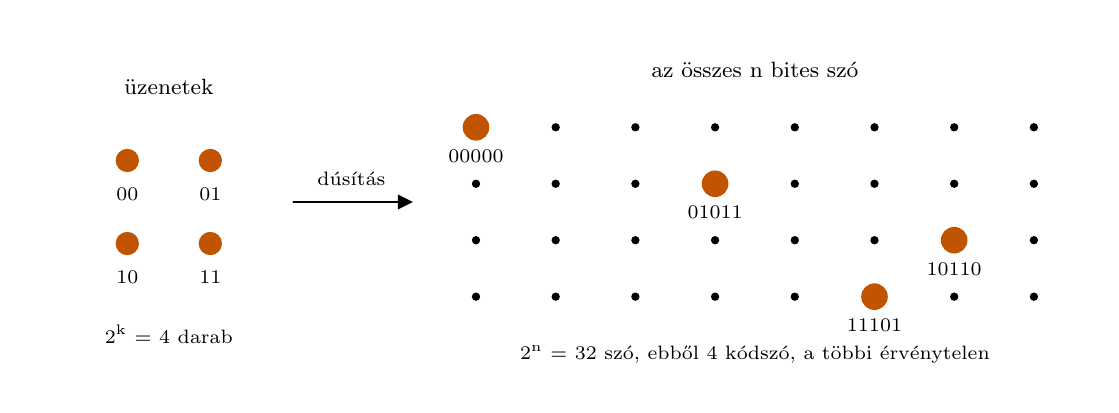
\begin{tikzpicture}[x=0.02109cm,y=-0.02109cm,line cap=round,line join=round]
\useasboundingbox (0,0) rectangle (640,215);
\path[fill=cB,draw=none] (60,80) circle[radius=0.148cm];
\node[anchor=base,inner sep=0pt,font=\scriptsize] at (60,104) {00};
\path[fill=cB,draw=none] (110,80) circle[radius=0.148cm];
\node[anchor=base,inner sep=0pt,font=\scriptsize] at (110,104) {01};
\path[fill=cB,draw=none] (60,130) circle[radius=0.148cm];
\node[anchor=base,inner sep=0pt,font=\scriptsize] at (60,154) {10};
\path[fill=cB,draw=none] (110,130) circle[radius=0.148cm];
\node[anchor=base,inner sep=0pt,font=\scriptsize] at (110,154) {11};
\node[anchor=base,inner sep=0pt,font=\footnotesize] at (85,40) {üzenetek};
\node[anchor=base,inner sep=0pt,font=\scriptsize] at (85,190) {2\textsuperscript{k} = 4 darab};
\path[draw=black,line width=0.7pt] (160,105) -- (230,105);
\path[fill=black,draw=none] (232,105) -- (223,100.5) -- (223,109.5) -- cycle;
\node[anchor=base,inner sep=0pt,font=\scriptsize] at (195,95) {dúsítás};
\path[fill=cB,draw=none] (270,60) circle[radius=0.169cm];
\node[anchor=base,inner sep=0pt,font=\scriptsize] at (270,81) {00000};
\path[fill=black,draw=none] (318,60) circle[radius=0.053cm];
\path[fill=black,draw=none] (366,60) circle[radius=0.053cm];
\path[fill=black,draw=none] (414,60) circle[radius=0.053cm];
\path[fill=black,draw=none] (462,60) circle[radius=0.053cm];
\path[fill=black,draw=none] (510,60) circle[radius=0.053cm];
\path[fill=black,draw=none] (558,60) circle[radius=0.053cm];
\path[fill=black,draw=none] (606,60) circle[radius=0.053cm];
\path[fill=black,draw=none] (270,94) circle[radius=0.053cm];
\path[fill=black,draw=none] (318,94) circle[radius=0.053cm];
\path[fill=black,draw=none] (366,94) circle[radius=0.053cm];
\path[fill=cB,draw=none] (414,94) circle[radius=0.169cm];
\node[anchor=base,inner sep=0pt,font=\scriptsize] at (414,115) {01011};
\path[fill=black,draw=none] (462,94) circle[radius=0.053cm];
\path[fill=black,draw=none] (510,94) circle[radius=0.053cm];
\path[fill=black,draw=none] (558,94) circle[radius=0.053cm];
\path[fill=black,draw=none] (606,94) circle[radius=0.053cm];
\path[fill=black,draw=none] (270,128) circle[radius=0.053cm];
\path[fill=black,draw=none] (318,128) circle[radius=0.053cm];
\path[fill=black,draw=none] (366,128) circle[radius=0.053cm];
\path[fill=black,draw=none] (414,128) circle[radius=0.053cm];
\path[fill=black,draw=none] (462,128) circle[radius=0.053cm];
\path[fill=black,draw=none] (510,128) circle[radius=0.053cm];
\path[fill=cB,draw=none] (558,128) circle[radius=0.169cm];
\node[anchor=base,inner sep=0pt,font=\scriptsize] at (558,149) {10110};
\path[fill=black,draw=none] (606,128) circle[radius=0.053cm];
\path[fill=black,draw=none] (270,162) circle[radius=0.053cm];
\path[fill=black,draw=none] (318,162) circle[radius=0.053cm];
\path[fill=black,draw=none] (366,162) circle[radius=0.053cm];
\path[fill=black,draw=none] (414,162) circle[radius=0.053cm];
\path[fill=black,draw=none] (462,162) circle[radius=0.053cm];
\path[fill=cB,draw=none] (510,162) circle[radius=0.169cm];
\node[anchor=base,inner sep=0pt,font=\scriptsize] at (510,183) {11101};
\path[fill=black,draw=none] (558,162) circle[radius=0.053cm];
\path[fill=black,draw=none] (606,162) circle[radius=0.053cm];
\node[anchor=base,inner sep=0pt,font=\footnotesize] at (438,30) {az összes n bites szó};
\node[anchor=base,inner sep=0pt,font=\scriptsize] at (438,200) {2\textsuperscript{n} = 32 szó, ebből 4 kódszó, a többi érvénytelen};
\end{tikzpicture}\end{center}

A tábla jobb oldali rácsában két kódszó külön áll, négy egymás mellett [bizonytalan: nem hangzott el, hogy ez a túl közeli, rossz esetet mutatja].

\textbf{Hasonlóság, távolság:} Hamming-távolság (helyenként XOR, szóban elhangzott). Pozitív, szimmetrikus, eleget tesz a háromszög-egyenlőtlenségnek. \textbf{A kód jósága:} a legközelebbi kódszavak távolsága. $\mathbf c=(c_1,c_2,\dots,c_n)$, $\mathcal C$ a kód maga, $d(\mathbf c_1,\mathbf c_2)$ a két kódszó távolsága.

\par\noindent{\small\renewcommand{\arraystretch}{1.25}\begin{tabularx}{\linewidth}{@{}>{\raggedright\arraybackslash}X>{\raggedright\arraybackslash}X>{\raggedright\arraybackslash}X@{}}\toprule
(6.17) & undefined & a kódtávolság [a felirat takarva, valószínű alakja]\\
(6.18) & undefined & jelezhető hibák száma [takarva: „hibajelzés”]\\
(6.19) & undefined & javítható hibák száma [takarva: „hibajavítás”]\\
\bottomrule\end{tabularx}}\par

\subsection{\texorpdfstring{T4. Lineáris blokk-kódok és szindróma (tábla 10\ldots{}12)}{T4. Lineáris blokk-kódok és szindróma (tábla 10…12)}}\label{e6-linearis}
\textbf{Kódolás:} $\mathbf u\to\mathbf c\in\mathcal C$, $k$ bitből $n$ bit. \textbf{Hibamodell:} $\mathbf c\to\mathbf v(\mathbf c,\mathbf e)$. \textbf{Dekódolás:} $\mathbf v\to\hat{\mathbf c}\in\mathcal C\to\hat{\mathbf u}$ (a 10. táblán kalap nélkül $\mathbf u$ áll, a 11. táblán már $\hat{\mathbf u}$).

\textbf{Lineáris blokk-kódok.} Elemi műveletek mod 2 a $\{0,1\}$ elemhalmazon: $+$ (XOR), $\times$ (AND). \textbf{Lineáris kód:} $\mathcal C$ lineáris tér, ha $\mathbf c_1,\mathbf c_2\in\mathcal C$, akkor $\mathbf c_1+\mathbf c_2\in\mathcal C$. $\mathbf c_1+\mathbf c_1=\mathbf 0$, ezért $\mathbf 0\in\mathcal C$. \textbf{A generátormátrix elemei:} $\mathbf g_1,\mathbf g_2,\dots,\mathbf g_k$.

\par\noindent{\small\renewcommand{\arraystretch}{1.25}\begin{tabularx}{\linewidth}{@{}>{\raggedright\arraybackslash}X>{\raggedright\arraybackslash}X>{\raggedright\arraybackslash}X@{}}\toprule
(6.20) & undefined & a táblán: undefined, undefined, undefined\\
(6.21) & undefined & pl. undefined, undefined, undefined\\
(6.22) & undefined & undefined, a undefined sorai undefined\\
(6.23) & undefined & Segít, ha undefined \ldots{} [a sor vége kilóg a képből, koma szerint: szisztematikus]\\
(6.24) & undefined & \\
(6.25) & undefined & dekódolás\\
\bottomrule\end{tabularx}}\par

\begin{itemize}
\item \textbf{0)} szindrómatábla: $\mathbf s=\mathbf e\,\mathbf H^{\mathsf T}$
\item \textbf{1)} $\mathbf v_i\,\mathbf H^{\mathsf T}=\mathbf s_i$
\item \textbf{2)} dekódoló tábla: $\mathbf s_i\to\mathbf e_i$
\item \textbf{3)} $\hat{\mathbf c}=\mathbf v-\mathbf e$ (dekódolás, mod 2 ugyanaz, mint $\mathbf v+\mathbf e$)
\item \textbf{4)} $\hat{\mathbf c}\to\hat{\mathbf u}$ (a táblán fordított nyíl áll, lásd Javítások). $\hat{\mathbf c}$ csak becsült kódszó, ebből kell még az üzenet (szóban elhangzott).
\end{itemize}

Megjegyzések: a táblán a $\mathbf h_1,\dots,\mathbf h_{n-k}$ vektorok „hibavektorok” néven szerepelnek, de a jegyzetben a hibavektor csak $\mathbf e$, hogy egy szó egy dolgot jelentsen. A $\mathbf H$ mátrix a szakirodalomban paritásellenőrző mátrix [bizonytalan: az előadó elnevezése nem ismert]. A $\mathbf c\,\mathbf H^{\mathsf T}=\mathbf 0$ oka $\mathbf G\,\mathbf H^{\mathsf T}=\mathbf 0$, ez a táblán nem szerepel (koma: a $\mathbf h_i$ vektorok a $\mathbf G$ sorai által kifeszített térre merőleges teret alkotnak). A táblán a vektorokat egy, a mátrixokat két aláhúzás jelöli, a jegyzetben félkövér kis- és nagybetű.

\subsection{\texorpdfstring{T5. Jelölések és szóhasználat}{T5. Jelölések és szóhasználat}}\label{e6-jeloles}
\par\noindent{\small\renewcommand{\arraystretch}{1.25}\begin{tabularx}{\linewidth}{@{}>{\raggedright\arraybackslash}X>{\raggedright\arraybackslash}X>{\raggedright\arraybackslash}X@{}}\toprule
\textbf{Jel} & \textbf{Jelentés} & \textbf{Megjegyzés}\\\midrule
undefined, undefined & forrás ABC és elemszáma & tábla\\
undefined, undefined, undefined & szimbólum, kódszavának hossza, valószínűsége & a 2. táblán undefined, undefined\\
undefined, undefined & átlagos kódszóhossz szimbólumonként, illetve páronként & undefined\\
undefined & entrópia, bit/szimbólum & dőlt undefined, nem azonos a félkövér undefined mátrixszal\\
undefined & undefined & tábla 6\\
undefined & a bitek hibavalószínűsége (BSC) & index nélkül, undefined a szimbólumok valószínűsége\\
undefined & 0 küldve, 1 véve & [bizonytalan: az indexek sorrendje]\\
undefined & üzenet, kódszó, vett szó, hibavektor, szindróma & táblán egy aláhúzás\\
undefined, undefined, undefined & generátormátrix, paritásellenőrző mátrix, a szisztematikus alak jobb oldali része & táblán két aláhúzás\\
undefined & a kód, a kódszavak halmaza & táblán undefined\\
undefined, undefined & az üzenet és a kódszó bitszáma & \\
undefined, undefined, undefined & Hamming-távolság, kódtávolság, súly (egyesek száma) & undefined: kiegészítés\\
\bottomrule\end{tabularx}}\par

\par\noindent{\small\renewcommand{\arraystretch}{1.25}\begin{tabularx}{\linewidth}{@{}>{\raggedright\arraybackslash}X>{\raggedright\arraybackslash}X>{\raggedright\arraybackslash}X@{}}\toprule
\textbf{Szó (előadó)} & \textbf{Más forrásban} & \textbf{Jelentés}\\\midrule
prefixmentes kód & prefix kód (koma) & egyik kódszó sem eleje egy másiknak\\
azonnal dekódolható kód &  & minden kódszó végén rögtön dönthető, melyik szimbólum volt\\
egyértelműen visszaállítható, megfejthető & egyértelműen visszafejthető (koma) & minden bitsorozatnak legfeljebb egy felbontása van\\
törlődéses hiba, tévesztés &  & a vevő nem dönt, illetve rosszul dönt\\
kódtávolság & undefined & a legközelebbi kódszavak Hamming-távolsága\\
szindróma & szindrómavektor (koma) & undefined\\
\bottomrule\end{tabularx}}\par

% ------------------------------------------------------------------
\section{\texorpdfstring{6.1. feladat: Fix hosszú kód: 32 és 33 szimbólum}{6.1. feladat: Fix hosszú kód: 32 és 33 szimbólum}}\label{p6_01}
\setcounter{lepes}{0}
\begin{feladat}{6.1. feladat}
Egy forrás $N=32$, egy másik $N=33$ különböző szimbólumot ad ki. Mindkettőt fix hosszú bináris kóddal kódoljuk. Hány bites kódszó kell, és hány százalékkal hosszabb ez az elméleti $\log_2 N$ értéknél?

{\footnotesize\sffamily Forrás: Kódolás előadás, tábla 3 (kép 2268) $\cdot$ koma E2 $\cdot$ azonosító: p6\_01. Címkék: beugró, javítás}
\end{feladat}
\begin{keresunk}
\begin{itemize}
\item $L_1$ (kódszóhossz az első forrásnál), $L_2$ (kódszóhossz a második forrásnál) [bit/szimbólum]
\item a romlás százalékban
\end{itemize}
\end{keresunk}
\begin{jeloles}
\begin{jeltabla}
$\ca{N_1}$ & az első forrás szimbólumainak száma & $32$\,s\\
$\cb{N_2}$ & a második forrás szimbólumainak száma & $33$\,s\\
$L_1$ & kódszóhossz az első forrásnál & \emph{keresett}\\
$L_2$ & kódszóhossz a második forrásnál & \emph{keresett}\\
$N$ & a forrás szimbólumainak száma & \\
$L$ & átlagos kódszóhossz egy szimbólumra & \\
\end{jeltabla}
\par\smallskip\textbf{Adott még:}
\begin{itemize}
\item bináris kód, fix kódszóhossz
\end{itemize}
\end{jeloles}
\begin{elmelet}[Miért így? Egyszerűen]
\textbf{Miért $\log_2 N$ az elméleti érték?}\par Mert $L$ biten $2^L$ különböző szó írható fel. Ahhoz, hogy $N$ szimbólum mind külön szót kapjon, $2^L \ge N$ kell, vagyis $L \ge \log_2 N$.

\textbf{Miért kell felfelé kerekíteni?}\par Mert bitből csak egészet lehet küldeni. Ha $\log_2 N$ nem egész, a következő egész bitszám kell, különben valamelyik szimbólumnak nem jut szó.

\textbf{Miért pont a 33 a rossz eset?}\par Mert $33 = 2^5+1$: egyetlen szimbólum miatt kell a 6. bit, és az általa nyert újabb 32 szóból csak egy kell.
\end{elmelet}
\begin{elmelet}[Felhasznált elmélet]
\textbf{Fix hosszú kód.} $L$ bit $2^L$ szót ad, ezért (6.2):
\begin{center}\adjustbox{max width=\linewidth}{$\displaystyle L=\lceil\log_2N\rceil,\qquad \log_2N\le L<1+\log_2 N$}\end{center}

\end{elmelet}

\lepes{A szükséges bitszám 32 szimbólumra}
Megkeressük a legkisebb $L$ értéket, amelyre $2^L\ge N$.

\begin{center}\adjustbox{max width=\linewidth}{$\displaystyle 2^{L}\ge N$}\end{center}
\jegyzet{definíció}{minden szimbólumnak külön szó jusson}
\behely{\bh{\ca{N_1}}{\ca{32\un{s}}}}

\begin{center}\adjustbox{max width=\linewidth}{$\displaystyle 2^{5}={\ca{32}}\ge {\ca{32}}$}\end{center}
\jegyzet{behelyettesítés}{}

\begin{center}\adjustbox{max width=\linewidth}{$\displaystyle L_1=5\ \text{bit}$}\end{center}
\jegyzet{számérték}{$\log_2 32=5$ egész, nincs veszteség}

\lepes{A szükséges bitszám 33 szimbólumra}
Ugyanez a feltétel, de most az 5 bit már kevés.
\behely{\bh{\ca{N_1}}{\ca{32\un{s}}} \bh{\cb{N_2}}{\cb{33\un{s}}}}

\begin{center}\adjustbox{max width=\linewidth}{$\displaystyle 2^{5}={\ca{32}}<{\cb{33}}\le 64=2^{6}$}\end{center}
\jegyzet{behelyettesítés}{5 biten egy szimbólum kimaradna}

\begin{center}\adjustbox{max width=\linewidth}{$\displaystyle \log_2 {\cb{33}}=\frac{\ln {\cb{33}}}{\ln 2}$}\end{center}
\jegyzet{átalakítás}{áttérés természetes alapú logaritmusra}

\begin{center}\adjustbox{max width=\linewidth}{$\displaystyle \log_2 {\cb{33}}\approx 5{,}044$}\end{center}
\jegyzet{számérték}{}

\begin{center}\adjustbox{max width=\linewidth}{$\displaystyle L_2=\lceil 5{,}044\rceil=6\ \text{bit}$}\end{center}
\jegyzet{számérték}{}

\lepes{A romlás}
Összevetjük a tényleges hosszt az elméleti értékkel.

\begin{center}\adjustbox{max width=\linewidth}{$\displaystyle \text{romlás}=\frac{L-\log_2N}{\log_2N}$}\end{center}
\jegyzet{definíció}{}

\begin{center}\adjustbox{max width=\linewidth}{$\displaystyle \frac{6-5{,}044}{5{,}044}\approx 0{,}189=18{,}9\,\%$}\end{center}
\jegyzet{számérték}{az elméleti értékhez képest}

\begin{center}\adjustbox{max width=\linewidth}{$\displaystyle \frac{6-5}{5}=0{,}2=20\,\%$}\end{center}
\jegyzet{átalakítás}{a 32 szimbólumos esethez képest, így adja a tábla}

\lepes{Ellenőrzés a korláttal}
A (6.2) korlát mindkét esetben teljesül.

\begin{center}\adjustbox{max width=\linewidth}{$\displaystyle 5\le 5<6,\qquad 5{,}044\le 6<6{,}044$}\end{center}
\jegyzet{ellenőrzés}{}
\begin{figyelem}[Javítás]
A táblán (3. tábla, jobb oldali keret) „$N=32\to N=5$” és „$N=33\to N=6$” áll. A nyíl jobb oldalán a kódszóhossz van, helyesen $L=5$ és $L=6$. Az oktató a táblán nem javította.
\end{figyelem}
\begin{eredmeny}

\begin{center}\adjustbox{max width=\linewidth}{$\displaystyle L_1=5\ \text{bit},\qquad L_2=6\ \text{bit},\qquad \text{romlás}\approx 19\,\%\ \ (\text{kb. }20\,\%)$}\end{center}
\end{eredmeny}
\begin{tipp}[Ellenőrzés]
\begin{itemize}
\item Mértékegység: bit/szimbólum, egész szám, ahogy fix hosszú kódnál kell.
\item Határeset: $N=2^m$ esetén nincs romlás, $N=2^m+1$ esetén a legnagyobb.
\item Nagyságrend: 6 bit 64 szót ad, ebből 33 kell, a kapacitás fele kihasználatlan. Ez a romlás oka.
\end{itemize}
\end{tipp}
\begin{figyelem}[Tipikus hibák]
\begin{itemize}
\item $L=\log_2 33\approx 5{,}04$ bitet írnak, pedig fix hossznál csak egész bit lehet.
\item A romlást rossz alapra számolják. A tábla 20\%-a az 5 bithez, a 19\% a $\log_2 33$ értékhez viszonyít. Írd le, mihez viszonyítasz.
\end{itemize}
\end{figyelem}
\begin{tipp}[Saját számpélda (kiegészítés, a forrásban nem szerepel)]
\small
\begin{verbatim}
Angol ábécé, 26 betű: log2 26 = 4,700, L = 5 bit, romlás (5 - 4,700)/4,700 =
  6,4%.
Decimális számjegyek, 10 szimbólum: log2 10 = 3,322, L = 4 bit, romlás 20,4%.
\end{verbatim}
\end{tipp}
\begin{tipp}[Kapcsolat és analógia]

\par\noindent{\small\renewcommand{\arraystretch}{1.25}\begin{tabularx}{\linewidth}{@{}>{\raggedright\arraybackslash}X>{\raggedright\arraybackslash}X@{}}\toprule
6.2. példa & ugyanez a 33 szimbólum párokba szervezve, a romlás a felére csökken\\
A3 & a fix hosszú kód korlátja\\
\bottomrule\end{tabularx}}\par
\end{tipp}


% ------------------------------------------------------------------
\section{\texorpdfstring{6.2. feladat: Szimbólumpárok kódolása: 33 szimbólum}{6.2. feladat: Szimbólumpárok kódolása: 33 szimbólum}}\label{p6_02}
\setcounter{lepes}{0}
\begin{feladat}{6.2. feladat}
Egy forrás 33 különböző szimbólumot ad ki. A szimbólumait párosával kódoljuk, fix hosszú kóddal. Hány bites egy pár kódszava, mennyi az egy szimbólumra jutó átlagos kódszóhossz, és mennyi most a romlás?

{\footnotesize\sffamily Forrás: Kódolás előadás, tábla 3 (kép 2269, 2270) $\cdot$ koma E2 $\cdot$ azonosító: p6\_02. Címkék: beugró}
\end{feladat}
\begin{keresunk}
\begin{itemize}
\item $L^{(2)}$ (egy szimbólumpár kódszavának hossza) [bit/pár]
\item $L$ (átlagos kódszóhossz egy szimbólumra) [bit/szimbólum]
\item a romlás
\end{itemize}
\end{keresunk}
\begin{jeloles}
\begin{jeltabla}
$\ca{N}$ & a forrás szimbólumainak száma & $33$\\
$L^{(2)}$ & egy szimbólumpár kódszavának hossza & \emph{keresett}\\
$L$ & átlagos kódszóhossz egy szimbólumra & \emph{keresett}\\
$F$ & a forrás szimbólumainak halmaza ($\mathcal F^2$: a szimbólumpárok halmaza) & \\
\end{jeltabla}
\par\smallskip\textbf{Adott még:}
\begin{itemize}
\item párok kódolása fix hosszú kóddal
\end{itemize}
\end{jeloles}
\begin{elmelet}[Miért így? Egyszerűen]
\textbf{Miért segít a párosítás?}\par A felfelé kerekítés miatti veszteség (kevesebb mint 1 bit) most egy kódszóra jut, de a kódszó két szimbólumot visz. Egy szimbólumra így kevesebb mint fél bit veszteség jut.

\textbf{Miért $N^2$ szimbólumpár van?}\par Mert az első helyre $N$, a másodikra is $N$ szimbólum kerülhet, és minden kombináció előfordulhat.

\textbf{Miért osztunk kettővel a végén?}\par Mert az átlagos kódszóhossz egy forrásszimbólumra vonatkozik, a pár kódszava pedig kettőt hordoz.
\end{elmelet}
\begin{elmelet}[Felhasznált elmélet]
\textbf{Párok száma.} Minden kombináció külön pár:
\begin{center}\adjustbox{max width=\linewidth}{$\displaystyle \#\mathcal F^2=N^2$}\end{center}


\textbf{Párok kódszóhossza.} (6.4):
\begin{center}\adjustbox{max width=\linewidth}{$\displaystyle 2\log_2N\le L^{(2)}<1+2\log_2 N$}\end{center}

\end{elmelet}

\lepes{A párok száma}
Megszámoljuk, hány különböző szimbólumpár lehet.

\begin{center}\adjustbox{max width=\linewidth}{$\displaystyle \#\mathcal F^2={\ca{N}}^2$}\end{center}
\jegyzet{definíció}{}

\begin{center}\adjustbox{max width=\linewidth}{$\displaystyle {\ca{33}}^2=1089$}\end{center}
\jegyzet{számérték}{}

\lepes{A pár kódszavának hossza}
A legkisebb kettőhatványt keressük, amely legalább 1089.

\begin{center}\adjustbox{max width=\linewidth}{$\displaystyle 2^{10}=1024<1089\le 2048=2^{11}$}\end{center}
\jegyzet{behelyettesítés}{}

\begin{center}\adjustbox{max width=\linewidth}{$\displaystyle L^{(2)}=11\ \text{bit}$}\end{center}
\jegyzet{számérték}{$2\log_2 33\approx 10{,}09$ felfelé kerekítve}

\lepes{Egy szimbólumra jutó hossz}
A pár két szimbólumot visz, ezért kettővel osztunk.

\begin{center}\adjustbox{max width=\linewidth}{$\displaystyle L=\frac{L^{(2)}}{2}$}\end{center}
\jegyzet{átalakítás}{}

\begin{center}\adjustbox{max width=\linewidth}{$\displaystyle L=\frac{11}{2}=5{,}5\ \text{bit}$}\end{center}
\jegyzet{számérték}{}

\lepes{A romlás}
Összevetjük az elméleti $\log_2 {\ca{33}}\approx5{,}044$ bittel és a fix 5 bittel.

\begin{center}\adjustbox{max width=\linewidth}{$\displaystyle \frac{5{,}5-5{,}044}{5{,}044}\approx 0{,}090=9{,}0\,\%$}\end{center}
\jegyzet{számérték}{}

\begin{center}\adjustbox{max width=\linewidth}{$\displaystyle \frac{5{,}5-5}{5}=0{,}1=10\,\%$}\end{center}
\jegyzet{átalakítás}{így adja a tábla: „csak 10\%” romlás}

\lepes{A korlát egy szimbólumra}
A (6.4) korlátot kettővel osztjuk.

\begin{center}\adjustbox{max width=\linewidth}{$\displaystyle \log_2{\ca{N}}\le L<\tfrac12+\log_2{\ca{N}}$}\end{center}
\jegyzet{átalakítás}{}

\begin{center}\adjustbox{max width=\linewidth}{$\displaystyle 5{,}044\le 5{,}5<5{,}544$}\end{center}
\jegyzet{ellenőrzés}{teljesül}
\begin{eredmeny}

\begin{center}\adjustbox{max width=\linewidth}{$\displaystyle L^{(2)}=11\ \text{bit/pár},\qquad L=5{,}5\ \text{bit/szimbólum},\qquad \text{romlás}\approx 9\,\%$}\end{center}
\end{eredmeny}
\begin{tipp}[Ellenőrzés]
\begin{itemize}
\item Mértékegység: a pár kódszava bit/pár, az átlag bit/szimbólum.
\item Határeset: ha $N^2$ kettő hatványa, a romlás nulla.
\item Nagyságrend: 11 bit 2048 szót ad, ebből 1089 kell. A kihasználatlan rész egy szimbólumra vetítve kisebb, mint 6 bitnél.
\end{itemize}
\end{tipp}
\begin{figyelem}[Tipikus hibák]
\begin{itemize}
\item A 11 bitet adják meg végeredménynek, pedig az egy párra vonatkozik.
\item Azt hiszik, a párosítás mindig javít. Itt javít, de $N=32$ esetén nincs mit javítani.
\end{itemize}
\end{figyelem}
\begin{tipp}[Saját számpélda (kiegészítés, a forrásban nem szerepel)]
\small
\begin{verbatim}
Hármasával: 33? = 35 937, 2^15 = 32 768 < 35 937 <= 65 536 = 2^16.
L(3) = 16 bit, L = 16/3 = 5,333 bit, romlás (5,333 - 5,044)/5,044 = 5,7%.
\end{verbatim}
\end{tipp}
\begin{tipp}[Kapcsolat és analógia]

\par\noindent{\small\renewcommand{\arraystretch}{1.25}\begin{tabularx}{\linewidth}{@{}>{\raggedright\arraybackslash}X>{\raggedright\arraybackslash}X@{}}\toprule
6.1. példa & ugyanez a forrás szimbólumonként\\
6.5. példa & ugyanez a gondolat entrópiával: $H(\mathcal F^2)=2H(\mathcal F)$\\
\bottomrule\end{tabularx}}\par
\end{tipp}


% ------------------------------------------------------------------
\section{\texorpdfstring{6.3. feladat: McMillan-egyenlőtlenség: az a, b, c kód}{6.3. feladat: McMillan-egyenlőtlenség: az a, b, c kód}}\label{p6_03}
\setcounter{lepes}{0}
\begin{feladat}{6.3. feladat}
Három szimbólum kódja: $a \to 1$, $b \to 10$, $c \to 0$. a) Egyértelműen megfejthető a kód? Bontsuk fel a 10101010 sorozatot. b) Mi változik, ha $c \to 00$?

{\footnotesize\sffamily Forrás: Kódolás előadás, tábla 4 (kép 2273) $\cdot$ koma E2 $\cdot$ azonosító: p6\_03. Címkék: beugró}
\end{feladat}
\begin{keresunk}
\begin{itemize}
\item $\sum 2^{-l_i}$ mindkét változatra
\item a 10101010 felbontásai
\end{itemize}
\end{keresunk}
\begin{jeloles}
\begin{jeltabla}
$\ca{l_a}$ & az a kódszavának hossza & $1$\\
$\cb{l_b}$ & a b kódszavának hossza & $2$\\
$\cc{l_c}$ & a c kódszavának hossza & $1$\\
$l_i$ & az i-edik kódszó hossza & \emph{keresett}\\
$a$ & az első szimbólum & \\
$b$ & a második szimbólum & \\
$c$ & a harmadik szimbólum & \\
$l_3$ & kódszóhossz & \\
\end{jeltabla}
\par\smallskip\textbf{Adott még:}
\begin{itemize}
\item vett sorozat: 10101010
\end{itemize}
\end{jeloles}
\begin{elmelet}[Miért így? Egyszerűen]
\textbf{Miért elég összeadni a $2^{-l_i}$ tagokat?}\par Mert a McMillan-egyenlőtlenség szerint minden egyértelműen megfejthető kód hosszaira $\sum 2^{-l_i}\le 1$. Ha az összeg nagyobb, a kód biztosan rossz, és ehhez magukat a kódszavakat meg sem kell nézni.

\textbf{Miért nem elég, ha az összeg legfeljebb 1?}\par Mert a feltétel csak a hosszakról szól. Azt mondja meg, hogy ilyen hosszakkal lehet jó kódot csinálni, de egy konkrét kód ettől még lehet rossz.

\textbf{Miért pont a 10101010 a jó próba?}\par Mert benne a $10$ kódszó és az $a\,c$ sorozat (1, majd 0) betűre ugyanaz. Ahol ez a kétféle olvasat lehetséges, ott a kód kétértelmű.
\end{elmelet}
\begin{elmelet}[Felhasznált elmélet]
\textbf{McMillan-egyenlőtlenség.} Egyértelműen megfejthető kódra (6.5):
\begin{center}\adjustbox{max width=\linewidth}{$\displaystyle \sum_{i=1}^{N}2^{-l_i}\le 1$}\end{center}


\textbf{Kraft-egyenlőtlenség.} Ha a feltétel teljesül, létezik ilyen hosszú prefixmentes kód (A5).
\end{elmelet}

\lepes{Az összeg az első változatra}
Kiszámoljuk a McMillan-összeget a hosszakból.

\begin{center}\adjustbox{max width=\linewidth}{$\displaystyle \sum 2^{-l_i}=2^{-1}+2^{-2}+2^{-1}$}\end{center}
\jegyzet{tétel}{McMillan}

\begin{center}\adjustbox{max width=\linewidth}{$\displaystyle \tfrac12+\tfrac14+\tfrac12=1{,}25>1$}\end{center}
\jegyzet{számérték}{nem teljesül}

\lepes{Következtetés}
Ha a feltétel sérül, a kód nem lehet egyértelműen megfejthető.

\begin{center}\adjustbox{max width=\linewidth}{$\displaystyle 1{,}25>1\ \Longrightarrow\ \text{nem egyértelműen megfejthető}$}\end{center}
\jegyzet{tétel}{}

\lepes{Kétértelmű sorozat}
Konkrétan is megmutatjuk: a 10101010 többféleképp bontható fel.

\begin{center}\adjustbox{max width=\linewidth}{$\displaystyle 10\,|\,10\,|\,10\,|\,10 = b\,b\,b\,b$}\end{center}
\jegyzet{behelyettesítés}{}

\begin{center}\adjustbox{max width=\linewidth}{$\displaystyle 1\,|\,0\,|\,1\,|\,0\,|\,1\,|\,0\,|\,1\,|\,0=a\,c\,a\,c\,a\,c\,a\,c$}\end{center}
\jegyzet{behelyettesítés}{}

\begin{center}\adjustbox{max width=\linewidth}{$\displaystyle 2^4=16\ \text{felbontás}$}\end{center}
\jegyzet{számérték}{mind a négy $10$ lehet $b$ vagy $a\,c$}

\lepes{A javított változat}
A táblán a $c$ kódszava $00$ lett, így $l_3=2$.

\begin{center}\adjustbox{max width=\linewidth}{$\displaystyle 2^{-1}+2^{-2}+2^{-2}=\tfrac12+\tfrac14+\tfrac14=1\le 1$}\end{center}
\jegyzet{behelyettesítés}{a tábla sora}

\begin{center}\adjustbox{max width=\linewidth}{$\displaystyle \text{a feltétel teljesül}$}\end{center}
\jegyzet{tétel}{a Kraft-tétel szerint létezik ilyen hosszú prefixmentes kód}

\lepes{Prefixmentes kód ugyanezekkel a hosszakkal}
A tábla jobb szélén: $a\to1$, $b\to00$, $c\to01$.

\begin{center}\adjustbox{max width=\linewidth}{$\displaystyle 1,\ 00,\ 01:\ \text{egyik sem eleje a másiknak}$}\end{center}
\jegyzet{ellenőrzés}{azonnal dekódolható}
\begin{eredmeny}

\begin{center}\adjustbox{max width=\linewidth}{$\displaystyle \{1,10,0\}:\ \sum 2^{-l_i}=1{,}25>1,\qquad \{1,10,00\}\ \text{és}\ \{1,00,01\}:\ \sum 2^{-l_i}=1$}\end{center}
\end{eredmeny}
\begin{tipp}[Ellenőrzés]
\begin{itemize}
\item A 16 felbontást a független szkript számolta, minden lehetséges darabolást végignézve.
\item Határeset: ha minden kódszó 1 bites, legfeljebb 2 szimbólum fér el ($2\cdot\tfrac12=1$).
\item Sardinas és Patterson tesztje (kiegészítés) szerint az első kód nem, a második és a harmadik egyértelműen megfejthető.
\end{itemize}
\end{tipp}
\begin{figyelem}[Tipikus hibák]
\begin{itemize}
\item A feltétel teljesülését a kód helyességének hiszik. Az $\{1,10,00\}$ kód nem az összegtől jó, hanem a szerkezetétől: bár az $1$ eleje a $10$-nek, a $00$ miatt mindig csak egyféleképpen bontható fel, csak nem azonnal.
\item Elfelejtik, hogy a McMillan-feltétel csak szükséges: ha teljesül, a konkrét kódot még külön meg kell vizsgálni.
\end{itemize}
\end{figyelem}
\begin{tipp}[Kapcsolat és analógia]

\par\noindent{\small\renewcommand{\arraystretch}{1.25}\begin{tabularx}{\linewidth}{@{}>{\raggedright\arraybackslash}X>{\raggedright\arraybackslash}X@{}}\toprule
6.4. példa & a javított $\{1,10,00\}$ kód dekódolása\\
koma G3/3 & a „Pisti kód”: a hosszak jók, a kód mégsem prefixmentes\\
\bottomrule\end{tabularx}}\par
\end{tipp}


% ------------------------------------------------------------------
\section{\texorpdfstring{6.4. feladat: Egyértelmű, de nem azonnal dekódolható kód}{6.4. feladat: Egyértelmű, de nem azonnal dekódolható kód}}\label{p6_04}
\setcounter{lepes}{0}
\begin{feladat}{6.4. feladat}
A kód: $a\to1$, $b\to10$, $c\to00$. A vett sorozat: 1011110000001. Dekódold! Azonnal dekódolható a kód?

{\footnotesize\sffamily Forrás: Kódolás előadás, tábla 4 (kép 2273) $\cdot$ koma E2 (javítva) $\cdot$ azonosító: p6\_04. Címkék: nehezebb, javítás}
\end{feladat}
\begin{keresunk}
\begin{itemize}
\item a dekódolt szimbólumsorozat
\item azonnal dekódolható a kód?
\end{itemize}
\end{keresunk}
\begin{jeloles}
\begin{jeltabla}
$a$ & az első szimbólum & \\
$b$ & a második szimbólum & \\
$c$ & a harmadik szimbólum & \\
\end{jeltabla}
\par\smallskip\textbf{Adott még:}
\begin{itemize}
\item kódszavak: $1$, $10$, $00$
\item vett sorozat: $1011110000001$ (13 bit)
\end{itemize}
\end{jeloles}
\begin{elmelet}[Miért így? Egyszerűen]
\textbf{Miért nem azonnal dekódolható?}\par Mert az $1$ kódszó eleje a $10$ kódszónak. Egy egyes után még nem tudjuk, hogy kész $a$ jött, vagy egy $b$ első bitje. Ezt csak a következő bitek döntik el, néha sok bittel később.

\textbf{Akkor miért mégis egyértelmű?}\par Mert a kód visszafelé olvasva prefixmentes: a kódszavak megfordítva $1$, $01$, $00$, és ezek közül egyik sem eleje a másiknak. A sorozatot hátulról olvasva minden lépésben biztosan dönthetünk (kiegészítés, a táblán nem szerepel).

\textbf{Miért érdemes a végéről kezdeni?}\par Mert hátulról nézve a kód azonnal dekódolható, előlről nem. A felbontás ezért egyértelmű, csak előlről nem látszik rögtön.
\end{elmelet}
\begin{elmelet}[Felhasznált elmélet]
\textbf{Prefixmentes kód.} Egyik kódszó sem eleje egy másiknak, ekkor azonnal dekódolható (A2).

\textbf{Egyértelmű megfejthetőség.} Minden bitsorozatnak legfeljebb egy felbontása van.
\end{elmelet}

\lepes{Hátulról olvasva}
A sorozat végén $1$ áll. Ez csak $a$ lehet, mert $b=10$ nullára végződik.

\begin{center}\adjustbox{max width=\linewidth}{$\displaystyle \dots 0\,|\,1 \ \Rightarrow\ a$}\end{center}
\jegyzet{behelyettesítés}{}

\begin{center}\adjustbox{max width=\linewidth}{$\displaystyle \dots 00\,|\,00\,|\,00\,|\,1 \ \Rightarrow\ c\,c\,c\,a$}\end{center}
\jegyzet{behelyettesítés}{hat nulla páronként: három $c$}

\lepes{A maradék eleje}
Maradt $101111$. A végén álló egyesek egyenként $a$, mert utánuk nincs nulla, ami $b$ vége lehetne.

\begin{center}\adjustbox{max width=\linewidth}{$\displaystyle 10\,|\,1\,|\,1\,|\,1\,|\,1$}\end{center}
\jegyzet{behelyettesítés}{az elején álló $10$ csak $b$ lehet}

\begin{center}\adjustbox{max width=\linewidth}{$\displaystyle b\,a\,a\,a\,a$}\end{center}
\jegyzet{számérték}{}

\lepes{A csapda előlről olvasva}
Ha a hatodik és a hetedik bitet (a táblán felülvonással jelölve) $b$ kódszónak olvassuk, zsákutcába jutunk.

\begin{center}\adjustbox{max width=\linewidth}{$\displaystyle 10\,|\,1\,|\,1\,|\,1\,|\,\overline{1\,0}\,|\,000001$}\end{center}
\jegyzet{behelyettesítés}{a 6. és 7. bit $b$ lenne}

\begin{center}\adjustbox{max width=\linewidth}{$\displaystyle 00\,|\,00\,|\,01\ ?$}\end{center}
\jegyzet{ellenőrzés}{a végén $01$ marad, ez nem kódszó}

\begin{center}\adjustbox{max width=\linewidth}{$\displaystyle b\,a\,a\,a\,a\,c\,c\,c\,a$}\end{center}
\jegyzet{számérték}{az egyetlen jó felbontás}

\lepes{Azonnal dekódolható?}
Megnézzük a prefixfeltételt.

\begin{center}\adjustbox{max width=\linewidth}{$\displaystyle 1\ \text{eleje a}\ 10\ \text{kódszónak}$}\end{center}
\jegyzet{definíció}{a kód nem prefixmentes}

\begin{center}\adjustbox{max width=\linewidth}{$\displaystyle \text{egyértelmű, de nem azonnal dekódolható}$}\end{center}
\jegyzet{ellenőrzés}{szóban elhangzott}
\begin{figyelem}[Javítás]
Koma E2 jegyzete szerint ez a kód „nem egyértelműen visszafejthető”. Ez téves. Az előadáson elhangzott: egyértelműen megfejthető, csak nem dekódolható azonnal, sorban haladva. A független szkript is egyetlen felbontást talál.
\end{figyelem}
\begin{eredmeny}

\begin{center}\adjustbox{max width=\linewidth}{$\displaystyle 1011110000001\ \to\ b\,a\,a\,a\,a\,c\,c\,c\,a,\qquad \text{egyértelmű, de nem azonnal dekódolható}$}\end{center}
\end{eredmeny}
\begin{tipp}[Ellenőrzés]
\begin{itemize}
\item A független szkript az összes lehetséges darabolást végignézte: pontosan egy felbontás van.
\item Visszakódolás: $10\,1\,1\,1\,1\,00\,00\,00\,1$ egymás után írva 1011110000001 $\checkmark$.
\item A Kraft-összeg $\tfrac12+\tfrac14+\tfrac14=1$, a McMillan-feltétel teljesül.
\end{itemize}
\end{tipp}
\begin{figyelem}[Tipikus hibák]
\begin{itemize}
\item Mohó olvasás: mindig a leghosszabb illeszkedő kódszót választják, és a 6. és 7. bitet $b$ kódszónak veszik. Ez zsákutcába visz.
\item Azt mondják, nem prefixmentes, tehát nem egyértelmű. A prefixmentes kód mindig egyértelmű, de fordítva nem igaz.
\end{itemize}
\end{figyelem}
\begin{tipp}[Kapcsolat és analógia]

\par\noindent{\small\renewcommand{\arraystretch}{1.25}\begin{tabularx}{\linewidth}{@{}>{\raggedright\arraybackslash}X>{\raggedright\arraybackslash}X@{}}\toprule
6.3. példa & ugyanez a kód a McMillan-feltétel oldaláról\\
A2 & azonnal dekódolható, prefixmentes kód\\
\bottomrule\end{tabularx}}\par
\end{tipp}


% ------------------------------------------------------------------
\section{\texorpdfstring{6.5. feladat: Szimbólumpárok entrópiája}{6.5. feladat: Szimbólumpárok entrópiája}}\label{p6_05}
\setcounter{lepes}{0}
\begin{feladat}{6.5. feladat}
Mutassuk meg, hogy független szimbólumokból álló pár entrópiája az egyes szimbólum entrópiájának kétszerese: $H(\mathcal F^2)=2H(\mathcal F)$. Mi következik ebből az átlagos kódszóhosszra?

{\footnotesize\sffamily Forrás: Kódolás előadás, tábla 5 és 6 (kép 2274, 2276) $\cdot$ koma E2 $\cdot$ azonosító: p6\_05. Címkék: nehezebb, javítás}
\end{feladat}
\begin{keresunk}
\begin{itemize}
\item $H(\mathcal F^2)$ (a szimbólumpárok entrópiája)
\item az egy szimbólumra jutó átlagos kódszóhossz korlátja
\end{itemize}
\end{keresunk}
\begin{jeloles}
\begin{jeltabla}
$N$ & a forrás szimbólumainak száma & \\
$p_1$ & egy bit hibavalószínűsége & \\
$p_i$ & az i-edik szimbólum valószínűsége & \\
$p_j$ & a j-edik szimbólum valószínűsége & \\
$i$ & a pár első szimbólumának sorszáma & \\
$j$ & a pár második szimbólumának sorszáma & \\
$P$ & valószínűség & \\
$a_i$ & az i-edik szimbólum & \\
$a_j$ & a j-edik szimbólum & \\
$L^{(2)}$ & egy szimbólumpár kódszavának hossza & \\
$L^{(1)}$ & átlagos kódszóhossz egy szimbólumra & \\
\end{jeltabla}
\par\smallskip\textbf{Adott még:}
\begin{itemize}
\item $\mathcal F$ forrás, $N$ szimbólum, $p_1,\dots,p_N$
\item a szimbólumok egymástól függetlenek
\end{itemize}
\end{jeloles}
\begin{elmelet}[Miért így? Egyszerűen]
\textbf{Miért $p_i\,p_j$ a pár valószínűsége?}\par Mert feltesszük, hogy a szimbólumok egymástól függetlenek. Független eseményeknél az együttes valószínűség a szorzat. A függetlenség a táblán nincs kimondva, a $p_i\,p_j$ alakból következik.

\textbf{Miért bomlik szét a logaritmus?}\par Mert a logaritmus a szorzatot összeggé alakítja: $\log(xy)=\log x+\log y$. Ettől lesz a kettős összegből két külön, egyforma tag.

\textbf{Miért tűnik el a külső összeg?}\par Mert $\sum_j p_j=1$. Ezért $\sum_j p_j \sum_i p_i\,\mathrm{ld}\tfrac1{p_i}$ értéke egyszerűen $1\cdot H(\mathcal F)$.
\end{elmelet}
\begin{elmelet}[Felhasznált elmélet]
\textbf{Entrópia.} (6.9):
\begin{center}\adjustbox{max width=\linewidth}{$\displaystyle H(\mathcal F)=\sum_{i=1}^{N}p_i\,\mathrm{ld}\frac1{p_i}$}\end{center}


\textbf{Logaritmus azonosság.} Szorzat logaritmusa:
\begin{center}\adjustbox{max width=\linewidth}{$\displaystyle \mathrm{ld}(xy)=\mathrm{ld}\,x+\mathrm{ld}\,y$}\end{center}

\end{elmelet}

\lepes{A pár entrópiája definíció szerint}
A párok halmazára írjuk fel az entrópiát, a pár valószínűsége $p_ip_j$.

\begin{center}\adjustbox{max width=\linewidth}{$\displaystyle H(\mathcal F^2)=\sum_{i=1}^{N}\sum_{j=1}^{N}p_ip_j\,\mathrm{ld}\frac{1}{p_ip_j}$}\end{center}
\jegyzet{definíció}{függetlenség: $P(a_i,a_j)=p_ip_j$}

\lepes{A logaritmus szétbontása}
A szorzat logaritmusa összeg.

\begin{center}\adjustbox{max width=\linewidth}{$\displaystyle =\sum_{i=1}^{N}\sum_{j=1}^{N}p_ip_j\left[\mathrm{ld}\frac1{p_i}+\mathrm{ld}\frac1{p_j}\right]$}\end{center}
\jegyzet{átalakítás}{logaritmus azonosság}

\lepes{Két tagra bontás és kiemelés}
Az első tagban $p_j$, a másodikban $p_i$ nem függ a belső összeg futó indexétől, ezért kiemelhető.

\begin{center}\adjustbox{max width=\linewidth}{$\displaystyle =\sum_{j=1}^{N}p_j\sum_{i=1}^{N}p_i\,\mathrm{ld}\frac1{p_i}+\sum_{i=1}^{N}p_i\sum_{j=1}^{N}p_j\,\mathrm{ld}\frac1{p_j}$}\end{center}
\jegyzet{átalakítás}{kiemelés}

\begin{center}\adjustbox{max width=\linewidth}{$\displaystyle \sum_{i=1}^{N}p_i\,\mathrm{ld}\frac1{p_i}=H(\mathcal F),\qquad \sum_{j=1}^{N}p_j=1$}\end{center}
\jegyzet{definíció}{a táblán kapcsos zárójellel jelölve}

\lepes{Az eredmény}
Mindkét tag $1\cdot H(\mathcal F)$.

\begin{center}\adjustbox{max width=\linewidth}{$\displaystyle H(\mathcal F^2)=1\cdot H(\mathcal F)+1\cdot H(\mathcal F)=2H(\mathcal F)$}\end{center}
\jegyzet{számérték}{}

\lepes{Következmény a kódszóhosszra}
A párok kódjára a (6.9) korlát érvényes, utána egy szimbólumra osztunk.

\begin{center}\adjustbox{max width=\linewidth}{$\displaystyle 2H(\mathcal F)\le L^{(2)}<1+2H(\mathcal F)$}\end{center}
\jegyzet{tétel}{a tábla „Tehát” sora}

\begin{center}\adjustbox{max width=\linewidth}{$\displaystyle H(\mathcal F)\le L^{(1)}<\tfrac12+H(\mathcal F)$}\end{center}
\jegyzet{átalakítás}{osztás kettővel, $L^{(1)}=L^{(2)}/2$}
\begin{figyelem}[Javítás]
A táblán a második alakban $p_i\cdot p_i$ és $[\mathrm{ld}\,\tfrac1{p_i}+\mathrm{ld}\,\tfrac1{p_i}]$ áll. Helyesen $p_i\,p_j$ és $[\mathrm{ld}\,\tfrac1{p_i}+\mathrm{ld}\,\tfrac1{p_j}]$, mert $\mathrm{ld}\tfrac{1}{p_ip_j}=\mathrm{ld}\tfrac1{p_i}+\mathrm{ld}\tfrac1{p_j}$. Az $1+2H(\mathcal F)$ tagban a 2 vastagon át van írva, valószínűleg az oktató a táblán javította.
\end{figyelem}
\begin{eredmeny}

\begin{center}\adjustbox{max width=\linewidth}{$\displaystyle H(\mathcal F^2)=2H(\mathcal F),\qquad H(\mathcal F)\le L^{(1)}<\tfrac12+H(\mathcal F)$}\end{center}
\end{eredmeny}
\begin{tipp}[Ellenőrzés]
\begin{itemize}
\item Szimbolikusan (sympy, $N=3$, tetszőleges $p_1,p_2$ és $p_3=1-p_1-p_2$) az azonosság teljesül.
\item Számpéldán is: $p=(\tfrac12,\tfrac14,\tfrac18,\tfrac18)$ esetén $H=1{,}75$ bit, $H(\mathcal F^2)=3{,}5$ bit.
\item Határeset: ha egy szimbólum biztos ($p_1=1$), $H=0$, és a pár entrópiája is 0.
\end{itemize}
\end{tipp}
\begin{figyelem}[Tipikus hibák]
\begin{itemize}
\item A külső összeget nem veszik 1-nek, és $H^2$ jön ki $2H$ helyett.
\item A függetlenséget nem mondják ki. Ha a szimbólumok összefüggnek, $H(\mathcal F^2)<2H(\mathcal F)$, és a párosítás még többet nyer (kiegészítés).
\end{itemize}
\end{figyelem}
\begin{tipp}[Saját számpélda (kiegészítés, a forrásban nem szerepel)]
\small
\begin{verbatim}
p = (1/2, 1/4, 1/8, 1/8):
H = 1/2*1 + 1/4*2 + 2*1/8*3 = 1,75 bit
Prefixmentes kód: 0, 10, 110, 111, L = 1/2*1 + 1/4*2 + 2*1/8*3 = 1,75 bit = H
Párok: 16 pár, H(F^2) = 3,5 bit = 2 * 1,75 bit
\end{verbatim}
\end{tipp}
\begin{tipp}[Kapcsolat és analógia]

\par\noindent{\small\renewcommand{\arraystretch}{1.25}\begin{tabularx}{\linewidth}{@{}>{\raggedright\arraybackslash}X>{\raggedright\arraybackslash}X@{}}\toprule
6.2. példa & ugyanez fix hosszú kóddal: $L=L^{(2)}/2$\\
koma G3/1 & $H=L$, ha minden $p_i=2^{-l_i}$\\
\bottomrule\end{tabularx}}\par
\end{tipp}


% ------------------------------------------------------------------
\section{\texorpdfstring{6.6. feladat: Hibák egy 1000 bites blokkban, BSC}{6.6. feladat: Hibák egy 1000 bites blokkban, BSC}}\label{p6_06}
\setcounter{lepes}{0}
\begin{feladat}{6.6. feladat}
Bináris szimmetrikus csatornán $n=1000$ bitet küldünk, a bitek hibavalószínűsége $p=10^{-4}$, a hibák függetlenek. Mennyi annak a valószínűsége, hogy 0, 1, illetve 2 bit hibás? Hány hibás bit várható?

{\footnotesize\sffamily Forrás: Kódolás előadás, tábla 7 (kép 2277) $\cdot$ koma E2 (javítva) $\cdot$ azonosító: p6\_06. Címkék: beugró, javítás}
\end{feladat}
\begin{keresunk}
\begin{itemize}
\item $P(0)$ (annak valószínűsége, hogy egy bit sem hibás), $P(1)$ (annak valószínűsége, hogy pontosan 1 bit hibás), $P(2)$ (annak valószínűsége, hogy pontosan 2 bit hibás)
\item a hibás bitek várható száma
\end{itemize}
\end{keresunk}
\begin{jeloles}
\begin{jeltabla}
$\ca{n}$ & a kódszó hossza bitben & $1000$\,bit\\
$\cb{p}$ & egy bit hibavalószínűsége & $10$\\
$E$ & a hibás bitek számának várható értéke & \\
\end{jeltabla}
\par\smallskip\textbf{Adott még:}
\begin{itemize}
\item BSC, független hibák
\end{itemize}
\end{jeloles}
\begin{elmelet}[Miért így? Egyszerűen]
\textbf{Miért binomiális eloszlás?}\par Mert minden bit egymástól függetlenül, ugyanazzal a $p$ valószínűséggel romlik el. Ez $n$ független kísérlet, és a hibák száma binomiális eloszlású.

\textbf{Miért kell az $\binom{n}{k}$ szorzó?}\par Mert nem mindegy, hol van a hiba. $k$ hibás helyet $\binom{n}{k}$ féleképpen lehet kiválasztani, és mindegyik elrendezés ugyanolyan valószínű.

\textbf{Miért $(1-p)^{n-k}$?}\par Mert a többi $n-k$ bitnek hibátlannak kell lennie, mindegyiknek $1-p$ eséllyel.
\end{elmelet}
\begin{elmelet}[Felhasznált elmélet]
\textbf{Binomiális eloszlás.} $k$ hiba $n$ bitből (A6):
\begin{center}\adjustbox{max width=\linewidth}{$\displaystyle P(k)=\binom{n}{k}p^k(1-p)^{n-k}$}\end{center}


\textbf{Várható érték.} Binomiális eloszlásnál:
\begin{center}\adjustbox{max width=\linewidth}{$\displaystyle E=np$}\end{center}

\end{elmelet}

\lepes{Nulla hiba}
Mind az 1000 bitnek jónak kell lennie.

\begin{center}\adjustbox{max width=\linewidth}{$\displaystyle P(0)=(1-{\cb{p}})^{n}=(1-10^{-4})^{1000}$}\end{center}
\jegyzet{behelyettesítés}{}

\begin{center}\adjustbox{max width=\linewidth}{$\displaystyle (1-{\cb{p}})^{\ca{n}}\approx e^{-np}=e^{-0{,}1}$}\end{center}
\jegyzet{közelítés}{mert $\ln(1-p)\approx -p$, ha $p\ll1$}

\begin{center}\adjustbox{max width=\linewidth}{$\displaystyle P(0)\approx 0{,}9048$}\end{center}
\jegyzet{számérték}{a tábla értéke}

\lepes{Egy hiba}
Egy hibás hely ezerféleképpen választható.

\begin{center}\adjustbox{max width=\linewidth}{$\displaystyle P(1)=\binom{1000}{1}\,10^{-4}\,(1-10^{-4})^{999}$}\end{center}
\jegyzet{behelyettesítés}{}

\begin{center}\adjustbox{max width=\linewidth}{$\displaystyle P(1)\approx {\ca{1000}}\cdot10^{-4}\cdot 0{,}9049\approx 0{,}0905$}\end{center}
\jegyzet{számérték}{a tábla értéke}

\lepes{Két hiba}
Két hibás hely $\binom{1000}{2}=499\,500$ féleképpen választható.

\begin{center}\adjustbox{max width=\linewidth}{$\displaystyle P(2)=\binom{1000}{2}\,10^{-8}\,(1-10^{-4})^{998}$}\end{center}
\jegyzet{behelyettesítés}{}

\begin{center}\adjustbox{max width=\linewidth}{$\displaystyle P(2)\approx 499\,500\cdot10^{-8}\cdot0{,}9050\approx 0{,}0045$}\end{center}
\jegyzet{számérték}{a táblán befejezetlen}

\lepes{Várható hibaszám, legalább egy hiba}
Összevetjük koma állításával.

\begin{center}\adjustbox{max width=\linewidth}{$\displaystyle E=np={\ca{1000}}\cdot10^{-4}=0{,}1$}\end{center}
\jegyzet{tétel}{binomiális eloszlás várható értéke}

\begin{center}\adjustbox{max width=\linewidth}{$\displaystyle P(\ge1)=1-P(0)\approx 0{,}0952$}\end{center}
\jegyzet{számérték}{nagyjából minden 10. blokkban van hiba}
\begin{figyelem}[Javítás]
Koma E2 jegyzetében „1000 közül 5\ldots{}6 biztos hibás” áll. Ez téves: a hibás bitek várható száma $np=0{,}1$, és kb. 90\% eséllyel egyetlen hiba sincs. A tábla harmadik sora befejezetlen („$\cong$ 0,0\ldots{}”), a helyes érték 0,0045.
\end{figyelem}
\begin{eredmeny}

\begin{center}\adjustbox{max width=\linewidth}{$\displaystyle P(0)\approx0{,}9048,\qquad P(1)\approx0{,}0905,\qquad P(2)\approx0{,}0045,\qquad E=0{,}1\ \text{hibás bit}$}\end{center}
\end{eredmeny}
\begin{tipp}[Ellenőrzés]
\begin{itemize}
\item Összeg: $0{,}9048+0{,}0905+0{,}0045+0{,}00015\approx1$, a 3 hibánál több elhanyagolható.
\item Arány: $P(1)/P(0)\approx np=0{,}1$, $P(2)/P(1)\approx np/2=0{,}05$ $\checkmark$.
\item A független szkript a pontos binomiális értékeket adja: 0,90483, 0,09049, 0,00452.
\end{itemize}
\end{tipp}
\begin{figyelem}[Tipikus hibák]
\begin{itemize}
\item Elfelejtik az $\binom{n}{k}$ szorzót, és $P(1)=p(1-p)^{n-1}\approx 10^{-4}$ jön ki.
\item A várható értéket összekeverik a hibák biztos számával: átlagosan 0,1 hiba nem jelenti, hogy biztosan van hiba.
\end{itemize}
\end{figyelem}
\begin{tipp}[Saját számpélda (kiegészítés, a forrásban nem szerepel)]
\small
\begin{verbatim}
Ha p = 10??, akkor np = 1:
P(0) = 0,3677, P(1) = 0,3681, P(2) = 0,1840, P(legalább 1) = 0,632.
Egy hiba ugyanolyan valószínű, mint a hibátlan blokk, és a blokkok kb. 63%-a
  hibás.
\end{verbatim}
\end{tipp}
\begin{tipp}[Kapcsolat és analógia]

\par\noindent{\small\renewcommand{\arraystretch}{1.25}\begin{tabularx}{\linewidth}{@{}>{\raggedright\arraybackslash}X>{\raggedright\arraybackslash}X@{}}\toprule
6.7. példa & a hibás blokkok 95\%-ában pontosan 1 hiba van, ezért egy hiba javítása már sokat ér (kiegészítés)\\
A6 & a BSC modell\\
\bottomrule\end{tabularx}}\par
\end{tipp}


% ------------------------------------------------------------------
\section{\texorpdfstring{6.7. feladat: Kódtávolság: hány hibát jelez és javít a C(5,2) kód?}{6.7. feladat: Kódtávolság: hány hibát jelez és javít a C(5,2) kód?}}\label{p6_07}
\setcounter{lepes}{0}
\begin{feladat}{6.7. feladat}
A tábla kódjának négy kódszava: $00000$, $01011$, $10110$, $11101$. Mennyi a kódtávolság? Hány hibát jelez és hányat javít a kód?
\begin{center}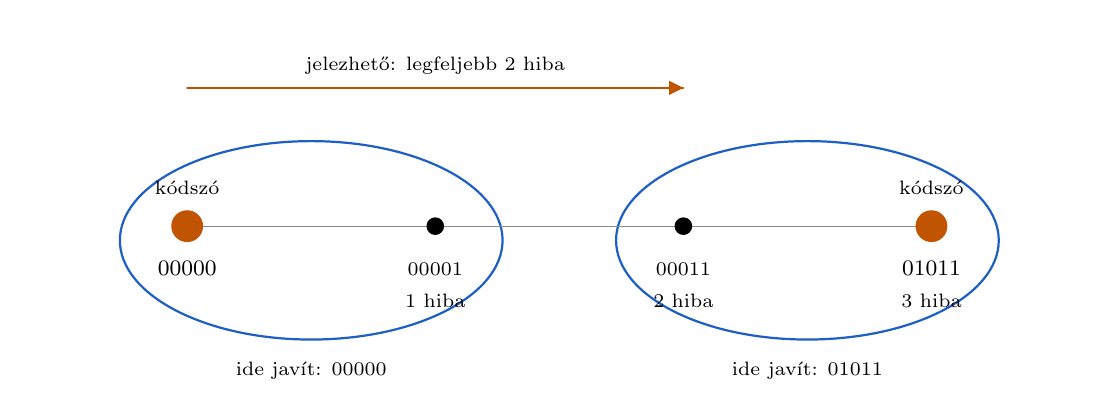
\begin{tikzpicture}[x=0.02250cm,y=-0.02250cm,line cap=round,line join=round]
\useasboundingbox (0,0) rectangle (600,205);
\path[draw=cA,line width=0.8pt] (160,120) ellipse[x radius=2.430cm,y radius=1.260cm];
\path[draw=cA,line width=0.8pt] (440,120) ellipse[x radius=2.430cm,y radius=1.260cm];
\path[draw=black!45,line width=0.35pt] (90,112) -- (510,112);
\path[fill=cB,draw=none] (90,112) circle[radius=0.202cm];
\node[anchor=base,inner sep=0pt,font=\footnotesize] at (90,140) {00000};
\path[fill=black,draw=none] (230,112) circle[radius=0.112cm];
\node[anchor=base,inner sep=0pt,font=\scriptsize] at (230,140) {00001};
\node[anchor=base,inner sep=0pt,font=\scriptsize] at (230,158) {1 hiba};
\path[fill=black,draw=none] (370,112) circle[radius=0.112cm];
\node[anchor=base,inner sep=0pt,font=\scriptsize] at (370,140) {00011};
\node[anchor=base,inner sep=0pt,font=\scriptsize] at (370,158) {2 hiba};
\path[fill=cB,draw=none] (510,112) circle[radius=0.202cm];
\node[anchor=base,inner sep=0pt,font=\footnotesize] at (510,140) {01011};
\node[anchor=base,inner sep=0pt,font=\scriptsize] at (510,158) {3 hiba};
\node[anchor=base,inner sep=0pt,font=\scriptsize] at (90,94) {kódszó};
\node[anchor=base,inner sep=0pt,font=\scriptsize] at (510,94) {kódszó};
\node[anchor=base,inner sep=0pt,font=\scriptsize] at (160,196) {ide javít: 00000};
\node[anchor=base,inner sep=0pt,font=\scriptsize] at (440,196) {ide javít: 01011};
\path[draw=cB,line width=0.8pt] (90,34) -- (370,34);
\path[fill=cB,draw=none] (370,34) -- (362,30) -- (362,38) -- cycle;
\node[anchor=base,inner sep=0pt,font=\scriptsize] at (230,24) {jelezhető: legfeljebb 2 hiba};
\end{tikzpicture}\end{center}


{\footnotesize\sffamily Forrás: Kódolás előadás, tábla 8, 9 és 12 (kép 2278, 2280, 2287) $\cdot$ koma E2, G6/5 $\cdot$ azonosító: p6\_07. Címkék: beugró}
\end{feladat}
\begin{keresunk}
\begin{itemize}
\item $d_{\min}$ (kódtávolság, két kódszó legkisebb eltérése)
\item a jelezhető és a javítható hibák száma
\end{itemize}
\end{keresunk}
\begin{jeloles}
\begin{jeltabla}
$\ca{n}$ & a kódszó hossza bitben & $5$\\
$\cb{k}$ & az üzenet hossza bitben & $2$\\
$d_{\min}$ & kódtávolság, két kódszó legkisebb eltérése & \emph{keresett}\\
$d$ & két kódszó Hamming-távolsága: hány helyen különböznek & \\
$w$ & egy kódszó súlya: az egyesek száma & \\
$c$ & egy kódszó & \\
\end{jeltabla}
\end{jeloles}
\begin{elmelet}[Miért így? Egyszerűen]
\textbf{Miért a legkisebb távolság számít?}\par Mert a hibák a legközelebbi két kódszó között okoznak bajt. Ha két kódszó $d$ távolságra van, $d$ hiba az egyiket a másikba viszi át, és ezt a vevő nem veheti észre.

\textbf{Miért $d_{\min}-1$ a jelezhető hibák száma?}\par Mert legfeljebb $d_{\min}-1$ hibától egy kódszó még nem ér el egy másik kódszót, tehát a vett szó érvénytelen, és ez feltűnik.

\textbf{Miért $\lfloor (d_{\min}-1)/2\rfloor$ a javítható hibák száma?}\par Mert javítani úgy lehet, hogy a legközelebbi kódszót választjuk. Ez akkor biztosan a jó, ha a hibás szó közelebb maradt az eredetihez, mint bármelyik máshoz, vagyis a távolság felénél kevesebbet tért el.
\end{elmelet}
\begin{elmelet}[Felhasznált elmélet]
\textbf{Hamming-távolság.} Ahány helyen különböznek, helyenként XOR (A7):
\begin{center}\adjustbox{max width=\linewidth}{$\displaystyle d(\mathbf a,\mathbf b)=w(\mathbf a+\mathbf b)$}\end{center}


\textbf{Kódtávolság.} (6.17) és (6.18), (6.19):
\begin{center}\adjustbox{max width=\linewidth}{$\displaystyle d_{\min}=\min_{\mathbf c_i\ne\mathbf c_j}d(\mathbf c_i,\mathbf c_j)$}\end{center}

\end{elmelet}

\lepes{Páronkénti távolságok}
Négy kódszóból hat pár van. Mindegyikre XOR, majd megszámoljuk az egyeseket.

\begin{center}\adjustbox{max width=\linewidth}{$\displaystyle d(00000,01011)=w(01011)=3$}\end{center}
\jegyzet{behelyettesítés}{}

\begin{center}\adjustbox{max width=\linewidth}{$\displaystyle d(00000,10110)=w(10110)=3$}\end{center}
\jegyzet{behelyettesítés}{}

\begin{center}\adjustbox{max width=\linewidth}{$\displaystyle d(00000,11101)=w(11101)=4$}\end{center}
\jegyzet{behelyettesítés}{}

\begin{center}\adjustbox{max width=\linewidth}{$\displaystyle d(01011,10110)=w(11101)=4$}\end{center}
\jegyzet{behelyettesítés}{}

\begin{center}\adjustbox{max width=\linewidth}{$\displaystyle d(01011,11101)=w(10110)=3$}\end{center}
\jegyzet{behelyettesítés}{}

\begin{center}\adjustbox{max width=\linewidth}{$\displaystyle d(10110,11101)=w(01011)=3$}\end{center}
\jegyzet{behelyettesítés}{}

\lepes{A kódtávolság}
A legkisebb érték.

\begin{center}\adjustbox{max width=\linewidth}{$\displaystyle d_{\min}=3$}\end{center}
\jegyzet{számérték}{}

\lepes{Jelzés és javítás}
Behelyettesítünk a (6.18) és (6.19) képletbe.

\begin{center}\adjustbox{max width=\linewidth}{$\displaystyle d_{\min}-1=2\ \text{hiba jelezhető}$}\end{center}
\jegyzet{tétel}{}

\begin{center}\adjustbox{max width=\linewidth}{$\displaystyle \left\lfloor\frac{3-1}{2}\right\rfloor=1\ \text{hiba javítható}$}\end{center}
\jegyzet{tétel}{}

\lepes{Gyorsabban, lineáris kódnál}
A páronkénti XOR mindig egy kódszót ad (linearitás), ezért elég a nemnulla kódszavak súlya.

\begin{center}\adjustbox{max width=\linewidth}{$\displaystyle d_{\min}=\min_{\mathbf c\ne\mathbf 0}w(\mathbf c)=\min(3,3,4)=3$}\end{center}
\jegyzet{átalakítás}{kiegészítés, a táblán nem szerepel}
\begin{eredmeny}

\begin{center}\adjustbox{max width=\linewidth}{$\displaystyle d_{\min}=3,\qquad 2\ \text{hibát jelez},\qquad 1\ \text{hibát javít}$}\end{center}
\end{eredmeny}
\begin{tipp}[Ellenőrzés]
\begin{itemize}
\item A független szkript minden kódszóra és minden 1, 2, 3 bites hibamintára kipróbálta: 2 hibáig minden hiba feltűnik, és 1 hiba mindig helyesen javul.
\item Az 1. lépésben a páronkénti XOR eredménye mindig a kód egy szava (linearitás).
\item Ugyanezt mutatja a szindrómatábla: a kód $mathbf H^{mathsf T}$ mátrixának öt sora (110, 011, 100, 010, 001) mind különböző és nemnulla, ezért mind az öt egybites hiba más szindrómát ad, és javítható.
\end{itemize}
\end{tipp}
\begin{figyelem}[Tipikus hibák]
\begin{itemize}
\item A $\lfloor d_{\min}/2\rfloor$ képletet használják (koma E2 így írja). Páros $d_{\min}$ esetén ez eggyel többet ad: $d_{\min}=4$ mellett 2 helyett csak 1 hiba javítható.
\item Jelzés és javítás egyszerre: ugyanaz a kód nem tud egyszerre 2 hibát jelezni és 1 hibát javítani. Ha 2 hiba van, a javító dekóder rossz kódszóra javít.
\end{itemize}
\end{figyelem}
\begin{tipp}[Saját számpélda (kiegészítés, a forrásban nem szerepel)]
\small
\begin{verbatim}
Ismétlő kód, 0000 és 1111: d_min = 4, 3 hibát jelez, ?3/2? = 1 hibát javít.
Két hibánál (0000 -> 1100) a vett szó mindkét kódszótól 2 távolságra van, nem
  dönthető el.
Ötszörös ismétlés, 00000 és 11111: d_min = 5, 4 hibát jelez, 2 hibát javít.
\end{verbatim}
\end{tipp}
\begin{tipp}[Kapcsolat és analógia]

\par\noindent{\small\renewcommand{\arraystretch}{1.25}\begin{tabularx}{\linewidth}{@{}>{\raggedright\arraybackslash}X>{\raggedright\arraybackslash}X@{}}\toprule
A7 & a városok analógiája\\
koma G3/4 & Golay (23, 12) kód: $d_{\min}=7$, 6 hibát jelez, hármat javít\\
\bottomrule\end{tabularx}}\par
\end{tipp}


% ------------------------------------------------------------------
\section{\texorpdfstring{6.8. feladat: Szindróma dekódolás: C(5,2), v = 11001}{6.8. feladat: Szindróma dekódolás: C(5,2), v = 11001}}\label{p6_08}
\setcounter{lepes}{0}
\begin{feladat}{6.8. feladat}
Egy szisztematikus lineáris blokk-kód generátormátrixa $\mathbf G=\begin{bmatrix}1&0&1&1&0\\0&1&0&1&1\end{bmatrix}$. a) Sorold fel a kódszavakat! b) Írd fel a $\mathbf H^{\mathsf T}$ mátrixot! c) A vett szó $\mathbf v=11001$. Dekódold!

{\footnotesize\sffamily Forrás: Kódolás előadás, tábla 10\ldots{}12 (kép 2281\ldots{}2287) $\cdot$ koma E2 $\cdot$ azonosító: p6\_08. Címkék: javítás}
\end{feladat}
\begin{keresunk}
\begin{itemize}
\item a kódszavak
\item $\mathbf H^{\mathsf T}$ (a paritásellenőrző mátrix transzponáltja)
\item $\hat{\mathbf e}$ (a becsült hibavektor), $\hat{\mathbf c}$ (a javított (becsült) kódszó), $\hat{\mathbf u}$ (a becsült üzenet)
\end{itemize}
\end{keresunk}
\begin{jeloles}
\begin{jeltabla}
$G$ & generátormátrix & \\
$B$ & a generátormátrix paritásrésze & \\
$\ca{n}$ & a kódszó hossza bitben & $5$\\
$\cb{k}$ & az üzenet hossza bitben & $2$\\
$v$ & a vett szó & \\
$\hat{\mathbf e}$ & a becsült hibavektor & \emph{keresett}\\
$\hat{\mathbf c}$ & a javított (becsült) kódszó & \emph{keresett}\\
$\hat{\mathbf u}$ & a becsült üzenet & \emph{keresett}\\
$u$ & az üzenet (2 bit) & \\
$c$ & a kódszó (5 bit) & \\
$u_1$ & az üzenet első bitje & \\
$g_1$ & a $\mathbf G$ első sora & \\
$u_2$ & az üzenet második bitje & \\
$g_2$ & a $\mathbf G$ második sora & \\
$I_3$ & 3$\times$3-as egységmátrix & \\
$s$ & szindróma & \\
$e$ & a hibavektor: ahol 1-es, ott romlott el a bit & \\
\end{jeltabla}
\end{jeloles}
\begin{elmelet}[Miért így? Egyszerűen]
\textbf{Miért szisztematikus a $\mathbf G$?}\par Mert az első két oszlopa az egységmátrix. Ezért a kódszó első $k$ bitje maga az üzenet, a maradék $n-k$ bit az ellenőrző rész. A dekódolás végén az üzenetet csak le kell olvasni.

\textbf{Miért éppen $\mathbf H^{\mathsf T}=[\mathbf B;\mathbf I]$?}\par Mert így $\mathbf G\mathbf H^{\mathsf T}=\mathbf I\mathbf B+\mathbf B\mathbf I=\mathbf B+\mathbf B=\mathbf 0$ mod 2. Ettől lesz minden kódszó szindrómája nulla.

\textbf{Miért elég a szindróma a hiba megtalálásához?}\par Mert $\mathbf s=\mathbf e\mathbf H^{\mathsf T}$ csak a hibától függ. Egy hibánál $\mathbf s$ éppen $\mathbf H^{\mathsf T}$ annak a sora, ahol a hiba van, így a szindróma megmutatja a hiba helyét.

\textbf{Miért a legkisebb súlyú hibát választjuk?}\par Mert kis $p$ mellett az egy hiba sokkal valószínűbb, mint a kettő: például $n=1000$, $p=10^{-4}$ esetén $P(1)approx0{,}09$, $P(2)approx0{,}0045$. Ugyanahhoz a szindrómához több hibaminta is tartozik, ezek közül a legvalószínűbbet vesszük.
\end{elmelet}
\begin{elmelet}[Felhasznált elmélet]
\textbf{Kódolás.} (6.20):
\begin{center}\adjustbox{max width=\linewidth}{$\displaystyle \mathbf c=\mathbf u\mathbf G$}\end{center}


\textbf{Szisztematikus alak.} (6.23):
\begin{center}\adjustbox{max width=\linewidth}{$\displaystyle \mathbf G=[\,\mathbf I_k\mid\mathbf B\,]\quad\Longrightarrow\quad \mathbf H^{\mathsf T}=\begin{bmatrix}\mathbf B\\\mathbf I_{n-k}\end{bmatrix}$}\end{center}


\textbf{Szindróma.} (6.22):
\begin{center}\adjustbox{max width=\linewidth}{$\displaystyle \mathbf s=\mathbf v\mathbf H^{\mathsf T}=\mathbf e\mathbf H^{\mathsf T}$}\end{center}

\end{elmelet}

\lepes{A kódszavak}
Minden $\mathbf u$ üzenetre $\mathbf c=\mathbf u\mathbf G$: azoknak a soroknak az összege, ahol $\mathbf u$ egyes.

\begin{center}\adjustbox{max width=\linewidth}{$\displaystyle \mathbf c=\mathbf u\mathbf G=u_1\mathbf g_1+u_2\mathbf g_2$}\end{center}
\jegyzet{definíció}{mod 2}

\begin{center}\adjustbox{max width=\linewidth}{$\displaystyle 00\to00000,\qquad 01\to01011,\qquad 10\to10110,\qquad 11\to11101$}\end{center}
\jegyzet{számérték}{$11$: $10110+01011=11101$}

\lepes{A H transzponált}
$\mathbf B$ alá az egységmátrix kerül.

\begin{center}\adjustbox{max width=\linewidth}{$\displaystyle \mathbf H^{\mathsf T}=\begin{bmatrix}1&1&0\\0&1&1\\1&0&0\\0&1&0\\0&0&1\end{bmatrix}$}\end{center}
\jegyzet{behelyettesítés}{felül $\mathbf B$, alul $\mathbf I_3$}

\begin{center}\adjustbox{max width=\linewidth}{$\displaystyle \mathbf G\mathbf H^{\mathsf T}=\mathbf B+\mathbf B=\mathbf 0$}\end{center}
\jegyzet{ellenőrzés}{minden kódszó szindrómája nulla}

\lepes{Szindrómatábla (0. lépés)}
Az egybites hibák szindrómái $\mathbf H^{\mathsf T}$ sorai.

\begin{center}\adjustbox{max width=\linewidth}{$\displaystyle \mathbf s=\mathbf e\mathbf H^{\mathsf T}$}\end{center}
\jegyzet{definíció}{}

\begin{center}\adjustbox{max width=\linewidth}{$\displaystyle 10000\to110,\qquad 01000\to011,\qquad 00100\to100,\qquad 00010\to010,\qquad 00001\to001$}\end{center}
\jegyzet{számérték}{mind különböző és nemnulla}

\lepes{A szindróma (1. lépés)}
$\mathbf v$ egyesei az 1., a 2. és az 5. helyen vannak, ezeket a sorokat adjuk össze (a táblán csillaggal jelölve).

\begin{center}\adjustbox{max width=\linewidth}{$\displaystyle \mathbf s=\mathbf v\mathbf H^{\mathsf T}=110+011+001$}\end{center}
\jegyzet{behelyettesítés}{mod 2}

\begin{center}\adjustbox{max width=\linewidth}{$\displaystyle \mathbf s=100\ne\mathbf 0$}\end{center}
\jegyzet{számérték}{hiba van}

\lepes{A hiba (2. lépés)}
A szindrómatáblából kikeressük.

\begin{center}\adjustbox{max width=\linewidth}{$\displaystyle \mathbf s=100\ \Longrightarrow\ \hat{\mathbf e}=00100$}\end{center}
\jegyzet{behelyettesítés}{a 3. bit hibás}

\lepes{A javított kódszó (3. lépés)}
Mod 2 a kivonás ugyanaz, mint az összeadás.

\begin{center}\adjustbox{max width=\linewidth}{$\displaystyle \hat{\mathbf c}=\mathbf v-\hat{\mathbf e}=\mathbf v+\hat{\mathbf e}$}\end{center}
\jegyzet{átalakítás}{}

\begin{center}\adjustbox{max width=\linewidth}{$\displaystyle \hat{\mathbf c}=11001+00100=11101$}\end{center}
\jegyzet{számérték}{}

\begin{center}\adjustbox{max width=\linewidth}{$\displaystyle \hat{\mathbf c}\mathbf H^{\mathsf T}=110+011+100+001=000$}\end{center}
\jegyzet{ellenőrzés}{valóban kódszó}

\lepes{Az üzenet (4. lépés)}
Szisztematikus kódnál az első ${\cb{k}}=2$ bit.

\begin{center}\adjustbox{max width=\linewidth}{$\displaystyle \hat{\mathbf u}=11$}\end{center}
\jegyzet{számérték}{szóban elhangzott}
\begin{figyelem}[Javítás]
A táblán a dekódolás 4. lépése „$\hat{\mathbf u}\to\hat{\mathbf c}$”. Helyesen $\hat{\mathbf c}\to\hat{\mathbf u}$: a javított kódszóból nyerjük ki az üzenetet. Az előadáson el is hangzott, hogy $\hat{\mathbf c}$ csak becsült kódszó, ebből kell még az üzenet.
\end{figyelem}
\begin{eredmeny}

\begin{center}\adjustbox{max width=\linewidth}{$\displaystyle \hat{\mathbf e}=00100,\qquad \hat{\mathbf c}=11101,\qquad \hat{\mathbf u}=11$}\end{center}
\end{eredmeny}
\begin{tipp}[Ellenőrzés]
\begin{itemize}
\item A javított szó szindrómája 000, tehát kódszó, és szerepel a kódszavak listájában.
\item Visszafelé: $\hat{\mathbf u}\mathbf G=11\cdot\mathbf G=11101=\hat{\mathbf c}$ $\checkmark$.
\item A független szkript (numpy, mod 2) ugyanezt adja, koma E2 eredménye is ez.
\end{itemize}
\end{tipp}
\begin{figyelem}[Tipikus hibák]
\begin{itemize}
\item A szindrómát $\mathbf H^{\mathsf T}$ sorai helyett oszlopaiból rakják össze, vagy elfelejtik, hogy a mod 2 összeadásban $1+1=0$.
\item $\hat{\mathbf c}$ értékét adják meg végeredménynek, pedig a kérdés az üzenet.
\end{itemize}
\end{figyelem}
\begin{tipp}[Saját számpélda (kiegészítés, a forrásban nem szerepel)]
\small
\begin{verbatim}
Ha v = 10110 érkezik: s = 110 + 100 + 010 = 000, tehát kódszó, ? = 10.
Ha v = 01111 érkezik: s = 011 + 100 + 010 + 001 = 100, ? = 00100, ? = 01011, ? =
  01.
\end{verbatim}
\end{tipp}
\begin{tipp}[Kapcsolat és analógia]

\par\noindent{\small\renewcommand{\arraystretch}{1.25}\begin{tabularx}{\linewidth}{@{}>{\raggedright\arraybackslash}X>{\raggedright\arraybackslash}X@{}}\toprule
6.7. példa & ugyanennek a kódnak a kódtávolsága: 1 hibát javít, ezért elég az egybites szindrómatábla\\
koma G6/5 & C(5,2) más $\mathbf B$ mátrixszal, $\mathbf v=10001$\\
koma G3/5 & (8,4) kód: előbb szisztematikussá kell alakítani\\
\bottomrule\end{tabularx}}\par
\end{tipp}

\section{Javítások}\label{j6}
J

\textbf{Javítások (6. fejezet)}\par
\#

A forrásokban talált hibák. Csendben semmit nem javítottunk: minden eltérés itt és a példánál is szerepel.

\par\noindent{\small\renewcommand{\arraystretch}{1.25}\begin{tabularx}{\linewidth}{@{}>{\raggedright\arraybackslash}X>{\raggedright\arraybackslash}X>{\raggedright\arraybackslash}X>{\raggedright\arraybackslash}X@{}}\toprule
\textbf{Hol} & \textbf{Mi állt ott} & \textbf{Helyesen} & \textbf{Miért}\\\midrule
Előadás, tábla 3 (kép 2268) & „undefined”, „undefined” & undefined, undefined & a nyíl jobb oldalán a kódszóhossz áll (6.1. példa)\\
Előadás, tábla 6 (kép 2276) & undefined & undefined & a pár valószínűsége undefined, és undefined két tagra bomlik (6.5. példa)\\
Előadás, tábla 11 (kép 2285) & 4) undefined & undefined & a javított kódszóból nyerjük ki az üzenetet, szóban is így hangzott el (6.8. példa)\\
Koma E2 & undefined & undefined & undefined, a tábla is szigorú egyenlőtlenséget ír\\
Koma E2 & az undefined kód „nem egyértelműen visszafejthető” & egyértelműen megfejthető, de nem azonnal dekódolható & egyetlen felbontás létezik (szkript), az előadáson is így hangzott el (6.4. példa)\\
Koma E2 & „1000 közül 5\ldots{}6 biztos hibás” & átlagosan 0,1 hibás bit, 90,5\% eséllyel egy sem & undefined (6.6. példa)\\
Koma E2 & javítani undefined bitet lehet & undefined & páros undefined esetén a félúton lévő szó egyforma messze van két kódszótól (6.7. példa)\\
\bottomrule\end{tabularx}}\par

\end{document}
